\documentclass[a4paper,12pt,oneside]{book}

\usepackage[utf8]{inputenc} % UTF-8
\usepackage[italian]{babel} %% Italiano

\usepackage{tocbibind} % Indice
\setcounter{tocdepth}{3}

\usepackage{listings}
\usepackage{multicol}

\usepackage{geometry}
\geometry{top=2cm,bottom=2.5cm,left=3.0cm,right=3.0cm} % Margini

\usepackage{titlesec}
\titleformat{\chapter}
  {\Large\bfseries} % format
  {}                % label
  {0pt}             % sep
  {\huge}           % before-code

\usepackage{fancyhdr}
\pagestyle{fancy}
\renewcommand{\headrulewidth}{0pt}
\fancyhf{}
\fancyhead[L]{}
\fancyfoot[C]{\thepage}

\usepackage{graphicx} % Required for inserting images
\usepackage{float}
\usepackage{subfig}
\newcommand*{\addheight}[2][.5ex]{%
  \raisebox{0pt}[\dimexpr\height+(#1)\relax]{#2}%
}

\usepackage{tabularx}
\usepackage{parskip}

\usepackage{minted}
\usepackage{xcolor}

\usepackage{setspace}
\singlespacing

% Inizio documento %

\begin{document}

% Frontespizio %
\begin{titlepage}
    \centering
    
    % Logo
    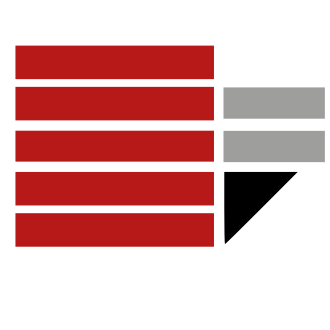
\includegraphics[width=0.3\textwidth]{assets/logo.png}\\[3cm]
    
    % Titolo
    {\huge\bfseries Ingegneria del Software}\\[0.5cm]
    
    % Sottotitolo
    {\Large Concetti di base, modelli di sviluppo e di testing, UML e Design Pattern}\\[0.5cm]

    % CdL
    {\small C.d.L Ingegneria Informatica - Cod. 0707}\\[0.5cm]
  
    \vfill
    
    % Data e versione
    {\large Versione 2.0}\hfill{\large \today}
        
\end{titlepage}

\tableofcontents

\chapter{Introduzione e concetti di base}

Gli obiettivi dell'ingegneria del software sono:
\begin{enumerate}
    \item Conoscere natura e qualità del software
    \item Saper rappresentare graficamente le fasi di sviluppo di progetto software
    \item Saper analizzare una soluzione progettuale (forza e debolezza)
    \item Sapersi muovere tra:
    \begin{itemize}
        \item Progettazione
        \item Implementazione
        \item Testing
        \item Manutenzione
    \end{itemize}
    \item Conoscenza delle metodologie di progettazione e sviluppo
\end{enumerate}

L'Ingegneria del Software si occupa di creare \textbf{sistemi software complessi} per cui è richiesto il lavoro di uno o più team.

Questi sistemi restano in \textit{vita} per diversi anni e subiscono modifiche allo scopo di:
\begin{enumerate}
    \item Eliminare difetti
    \item Migliorare caratteristiche
    \item Introdurre nuove funzionalità
    \item Rimuovere caratteristiche obsolete
\end{enumerate}

\begin{table}[H]
    \centering
    \begin{tabularx}{\textwidth}{|X|X|}
        \hline
        \textbf{Programmazione} & \textbf{Ingegneria del Software} \\
        \hline
        Scrittura di un programma completo & Progettazione e sviluppo di componenti che dovranno interagire tra loro (scritti anche da altri) \\
        \hline
        Attività individuale & Attività di gruppo \\
        \hline
    \end{tabularx}
    \caption{Definizione di Parnas}
\end{table}

\newpage

L'\textit{ingegnere del software} deve:
\begin{itemize}
    \item Saper programmare in uno o più linguaggi
    \item Avere familiarità con più approcci di progettazione
    \item Saper tradurre richieste vaghe in specifiche precise
    \item Sapere interagire con l'utente
    \item Districarsi attraverso diversi livelli di astrazione progettuale
    \item Saper costruire modelli e ragionarci al fine di scegliere un buon compromesso (\textit{trade-off})
    \item Saper operare all'interno di un team
\end{itemize}

\section{Ciclo di vita del software}
Costituito da diverse fasi (aventi come output un artefatto da trasmettere alla fase successiva) atte a sviluppare, implementare e consegnare un prodotto più affine possibile alle richieste del cliente.

\paragraph{Ciclo a cascata (Modello waterfall)}

\begin{enumerate}
    \item \textbf{Analisi e specifica dei requisiti}
    \begin{itemize}
        \item Definizione di costi e benefici della realizzazione del software
        \item Identificazione dei requisiti del sistema (espressi in una notazione formale comprensibile dal cliente)
        \item Attori: Cliente, Analisti di mercato, team di sviluppo
    \end{itemize}
    \item \textbf{Progettazione e specifica di sistema}, suddivisa in:
    \begin{itemize}
        \item \textit{Progettazione architetturale}: organizzazione del sistema in termini di componenti (di alto livello) e loro interazioni
        \item \textit{Progettazione di dettaglio}: scomposizione delle componenti in modulo di basso livello accuratamente definito
        \item Output: documento di specifica
    \end{itemize}
    \item \textbf{Codifica e test di modulo}
    \begin{itemize}
        \item Implementazione del sistema funzionante (composto da componenti progettati nelle fasi precedenti)
        \item Produzione di codice di test e successiva fase di test dei moduli
    \end{itemize}
    \item \textbf{Integrazione e test di sistema}: Integrazione e test dei moduli precedentemente sviluppati
    \item \textbf{Consegna e manutenzione}: Consegna al cliente e successiva fase di \textit{manutenzione} (raccolta di modifiche apportate al sistema dopo la sua consegna)
\end{enumerate}

\section{Natura e Qualità del software}

\subsection{Natura del software}

Prodotto dell'ingegneria del software: \textit{sistema software}

Distinto poiché \textit{duttile}: può essere direttamente modificato senza riconsiderare il progetto (rischioso).

Il costo del software è determinato da:
\begin{itemize}
    \item Progettazione
    \item Implementazione
    \item Manutenzione
\end{itemize}

\subsection{Qualità del software}

\textbf{Esterne}: visibili agli utenti del sistema.
\textbf{Interne}: visibili agli sviluppatori, importanti per il conseguimento delle esterne.

\begin{center}
  $\ast$~$\ast$~$\ast$
\end{center}

\paragraph{Correttezza} Un sistema software è \textit{corretto} soddisfa i requisiti (funzionali e non funzionali), espressi in maniera non ambigua. Valutabile tramite: testing e/o approcci analitici.

\paragraph{Affidabilità} Un sistema software è \textit{affidabile} se opera come previsto. Definita come \textit{probabilità che il sistema si comporti come attesa per un certo intervallo di tempo}. Affidabilità implica correttezza (ma non il contrario).

\paragraph{Robustezza} Un sistema software è \textit{robusto} se si comporta "bene" anche in casi non previsti dalle specifiche.

\paragraph{Prestazioni} Il livello di \textit{prestazioni} varia in base a: efficienza, risorse utilizzate, altro. È valutato tramite: misura, analisi di complessità e simulazione. Nel caso del processo di sviluppo prende il nome di \textbf{produttività}.

\paragraph{Usabilità} Un software è detto \textit{usabile} se è \textbf{user-friendly}. Dipende dall'implementazione dell'interfaccia.

\paragraph{Verificabilità} Un sistema software è \textit{verificabile} se è possibile verificarne correttezza e prestazioni. Può essere qualità esterna per sistemi critici. Svolta tramite analisi formale e testing o moduli di monitoraggio. Dipende da progettazione e linguaggi di programmazione.

\paragraph{Manutenibilità} Un sistema software è \textit{manutenibile} se è possibile: eliminare difetti, migliorare il funzionamento, introdurre nuove funzioni. È la qualità più costosa. Divisa in:
\begin{itemize}
    \item \textit{Adattiva}: modifiche richieste dall'ambiente esterno
    \item \textit{Correttiva}: eliminazione di errori
    \item \textit{Perfettiva}: interventi migliorativi o nuove funzioni
\end{itemize}

\paragraph{Riparabilità} Un sistema software è \textit{riparabile} se è possibile correggere difetti con quantità ragionevoli di lavoro. Dipende dalla modularità del software.

\paragraph{Evolvibilità} Un sistema software è \textit{evolvibile} se è capace di sostenere modifiche evolutive in maniera controllata e ordinata. Dipende dalle fasi di progettazione. È una qualità che si degrada all'aumentare delle iterazioni (modifiche).

\paragraph{Riusabilità} Un sistema software \textit{riusabile} se è possibile utilizzarne (una o più) parti per dare origine ad un altro prodotto (es. librerie), è un obiettivo della POO e si applica anche alle fasi di progettazione.

\paragraph{Portabilità} Un sistema software è \textit{portabile} se è possibile eseguirlo in ambienti (hardware o S.O.) diversi. È favorita dall'uso di linguaggi interpretati (es. Python, Java).

\paragraph{Comprensibilità} Un sistema software è \textit{comprensibile} in base alla complessità di progettazione e implementazione. Qualità che aiuta evolvibilità e verificabilità.

\paragraph{Interoperabilità} Un sistema software è \textit{interoperabile} se è capace di coesistere e/o cooperare con altri sistemi. Si raggiunge tramite l'uso di interfacce standard (es. plugin browser). Importante nei sistemi open-source.

\paragraph{Produttività} Un sistema software è più (o meno) \textit{produttivo} in base ad efficienza e prestazioni del processo di produzione. Influenzata dalla riusabilità.

\paragraph{Tempestività} Un sistema software è \textit{tempestivo} se è consegnato nei tempi previsti. Non è sempre una qualità. Un sistema software più completo consegnato in ritardo è meglio di un sistema incompleto consegnato in tempo. La consegna incrementale è una buona soluzione.

\paragraph{Visibilità} Un processo di sviluppo è \textit{visibile} se tutti i passi e lo stato corrente sono correttamente documentati. È fondamentale per valutare: azioni progettuali, variazioni del personale.

\newpage
\chapter{Principi dell'Ingegneria del Software}

Messi in pratica attraverso \textbf{metodologie}, costituite di:
\begin{itemize}
    \item \textbf{Metodi}: linee guida formali che regolano l'esecuzione di attività
    \item \textbf{Tecniche}: approcci di carattere meccanico e con limitata applicabilità
\end{itemize}

\section{Principi}

\paragraph{Rigore e formalità} (o \textit{rigorosità}) Si mantiene un certo livello di rigore per evitare imprecisioni e/o inaccuratezze. La formalità offre garanzie e vantaggi, ma aumenta la complessità progettuale.

\paragraph{Separazione degli interessi} Si separano gli aspetti progettuali così da potercisi concentrare singolarmente.
\begin{enumerate}
    \item \textbf{Separazione temporale} delle attività. Consente una pianificazione precisa ed evita inconvenienti legati al continuo cambiamento.
    \item \textbf{Separazione qualitativa} delle attività. Ad esempio \textit{correttezza} ed \textit{efficienza} possono essere considerate separatamente ed in maniera ordinata.
    \item \textbf{Separazione delle responsabilità}. Si suddividono i compiti tra le parti. Da qui deriva il principio di \textbf{modularità}
\end{enumerate}
In Java: metodi riusabili posti in classi di utilità apposite.

\paragraph{Modularità} Suddivisione di un sistema complesso in \textit{moduli}: parti più semplici (considerate come \textit{black-box}. Approcci:
\begin{itemize}
    \item \textbf{Bottom-Up}: si implementano i vari moduli e poi si integrano fra loro
    \item \textbf{Top-Down}: si scompone il problema in moduli e poi si progettano
\end{itemize}
Si tenta di raggiungere \textbf{alta coesione} e \textbf{basso accoppiamento}.
\begin{itemize}
    \item Coesione: connessione tra gli elementi che costituiscono il modulo
    \item Accoppiamento: relazione tra gli moduli
\end{itemize}

\paragraph{Astrazione} Consente di identificare gli aspetti fondamentali, tralasciando momentaneamente i dettagli progettuali/implementativi. Genera modelli formali (o semi-formali) che permettono di simulare e/o ragionare sul sistema. Esempio: \textit{interfacce} o \textit{classi astratte} di Java.

\paragraph{Anticipazione del cambiamento} Sta alla base di evolvibilità e riusabilità. Si predispone il progetto a possibili cambiamenti. Fondamentale nei processi (es. cambio di personale).

\paragraph{Generalità} Si cerca di risolvere il problema generico invece di quello specifico in favore di riusabilità. Va bilanciata rispetto a costi ed efficienza. Esempio: \textit{Collection Framework} di Java.

\paragraph{Incrementalità} Rilascio di versioni successive (risultato di processo evolutivo). Permette di raggiungere l'obiettivo attraverso approssimazioni consecutive.

\begin{figure}[H]
  \centering
  \subfloat[Alta coesione, basso accoppiamento]{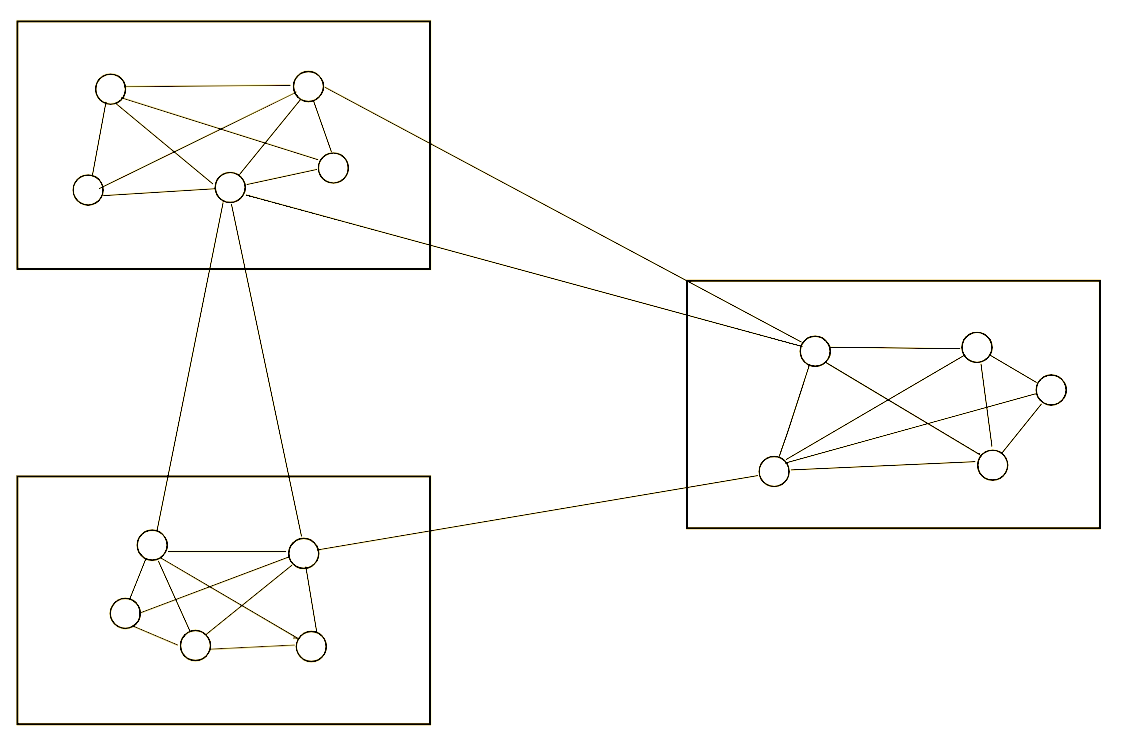
\includegraphics[width=0.48\textwidth]{assets/acba.png}}
  \hfill
  \subfloat[Forte accoppiamento]{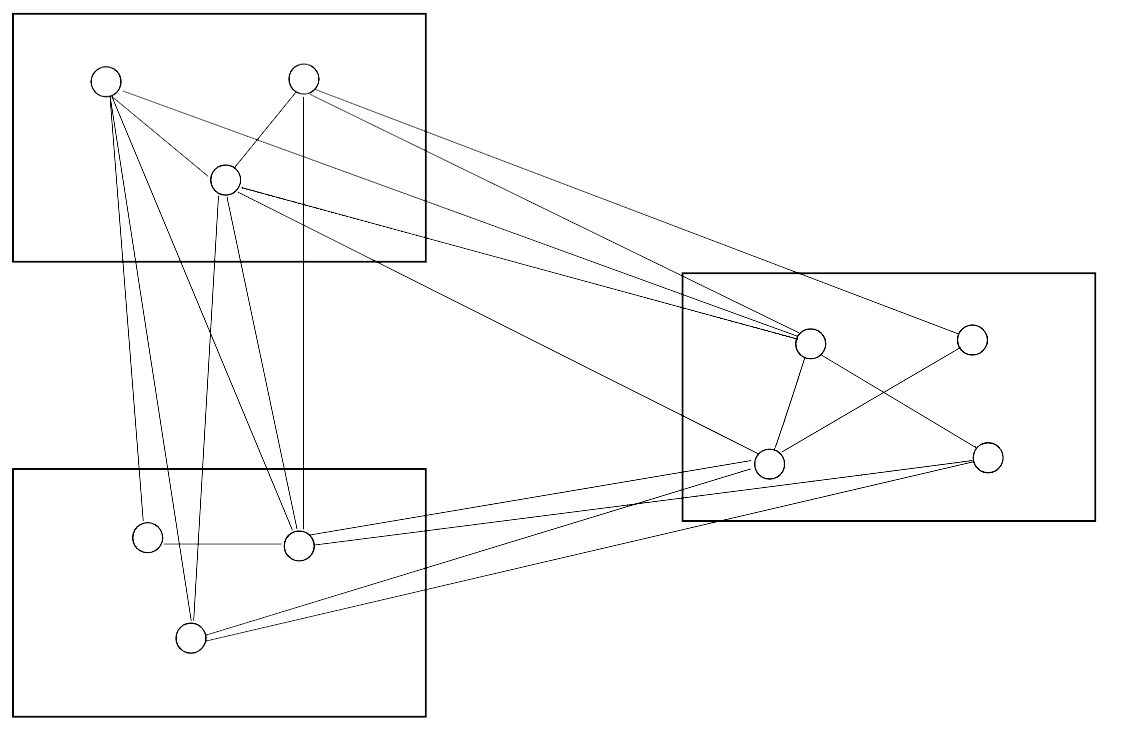
\includegraphics[width=0.48\textwidth]{assets/accopp.png}}
  \caption{Coesione e accoppiamento nei moduli}
\end{figure}

\section{Caso Studio - Compilatore}

Lo sviluppo di un compilatore segue metodi sistematici e formali di progettazione (spesso imposti da comitati - es. BNF, teoria degli automi). Applica i seguenti principi:
\begin{itemize}
    \item \textbf{Separazione degli interessi}, ci si concentra su efficienza e interfaccia.
    \item \textbf{Modularità}, il processo è scomposto in fasi: analisi lessicale, analisi sintattica (\textit{parsing}) e generazione di codice (intermedio $\rightarrow$ macchina)
    \item \textbf{Astrazione} tramite la generazione di codice intermedio (es. Java Bytecode)
    \item \textbf{Anticipazione del cambiamento} tramite l'utilizzo di librerie standard, ci si predispone a cambiamenti e/o estensioni.
    \item \textbf{Generalità} tramite codice intermedio per generalizzare (parametrizzare) l'architettura della macchina. La generazione stessa di compilatori è un processo automatizzato (tramite \textit{compiler compilers}).
    \item \textbf{Incrementalità} tramite versioning, permette: estensione della sintassi, migliori livelli di diagnostica, ottimizzazioni.
\end{itemize}

\begin{figure}
    \centering
    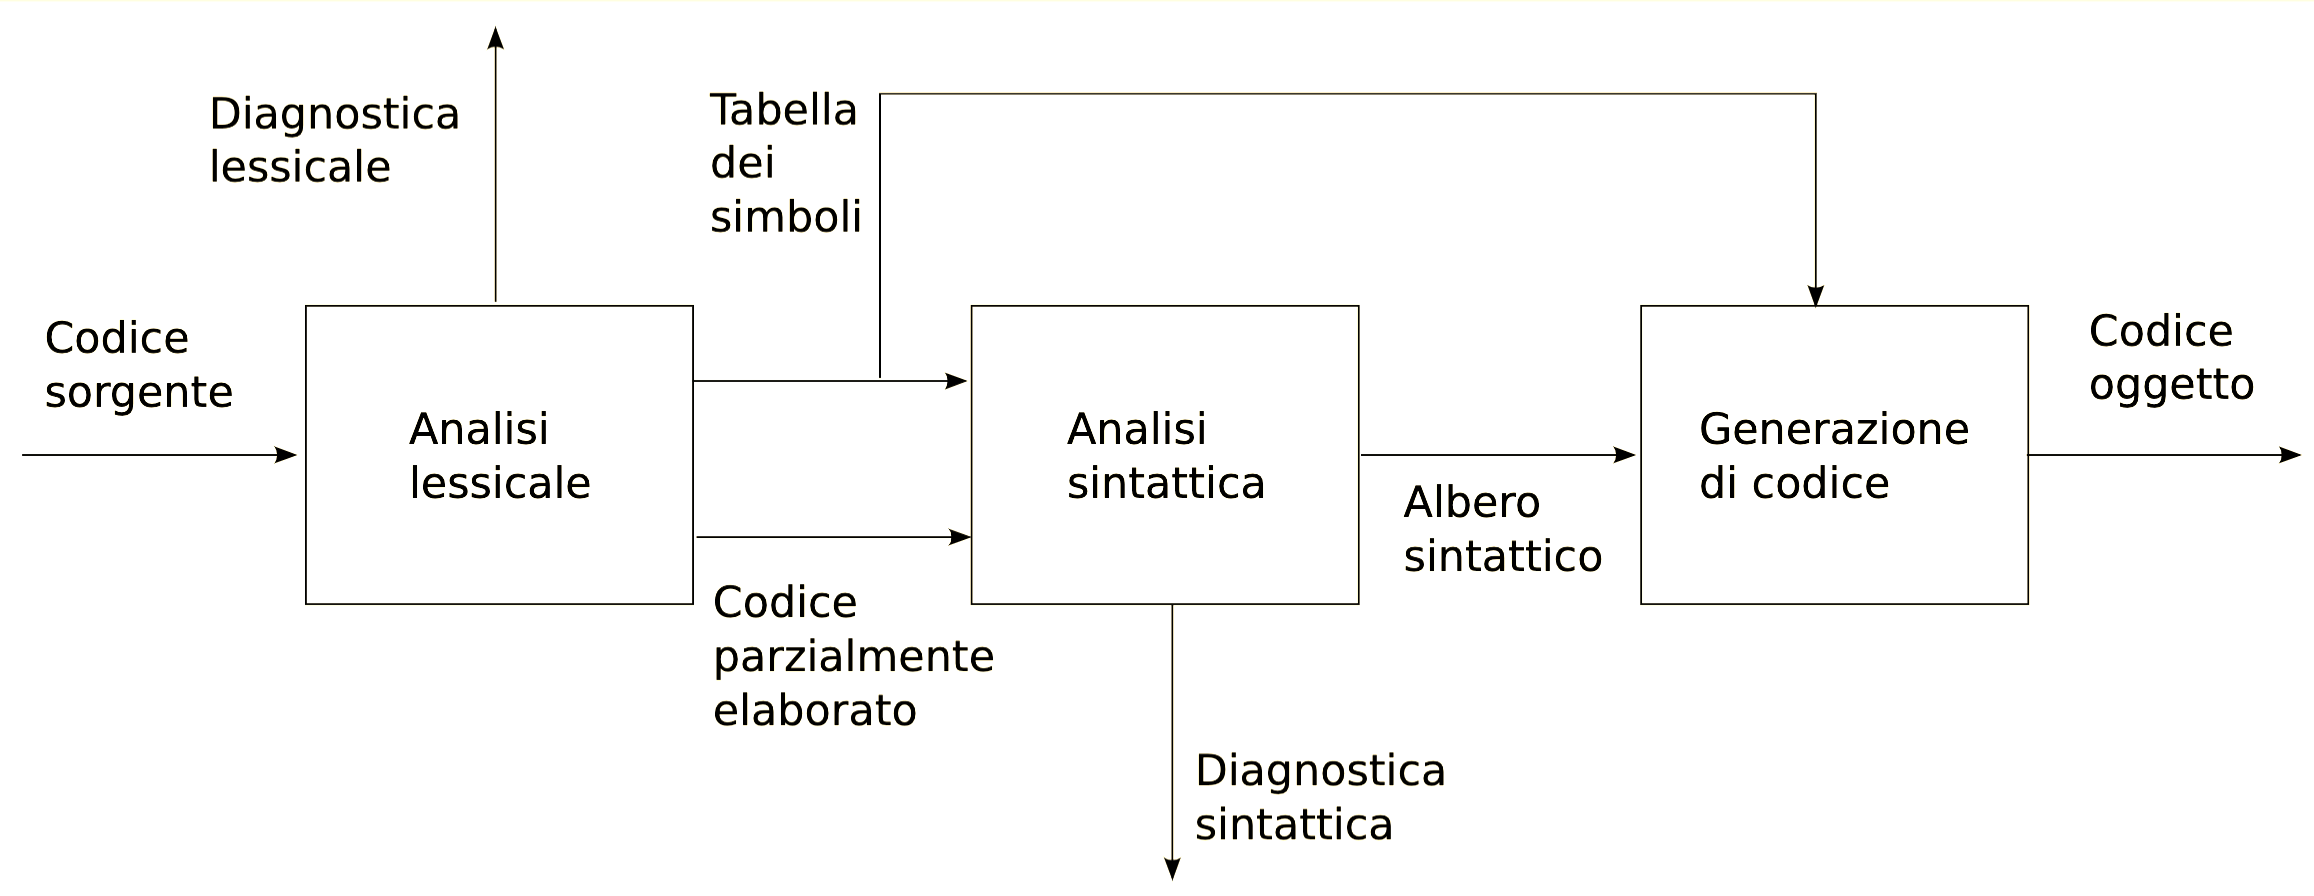
\includegraphics[width=1\linewidth]{assets/compilatore.png}
    \caption{Rappresentazione della struttura modulare del compilatore}
\end{figure}

\begin{figure}
    \centering
    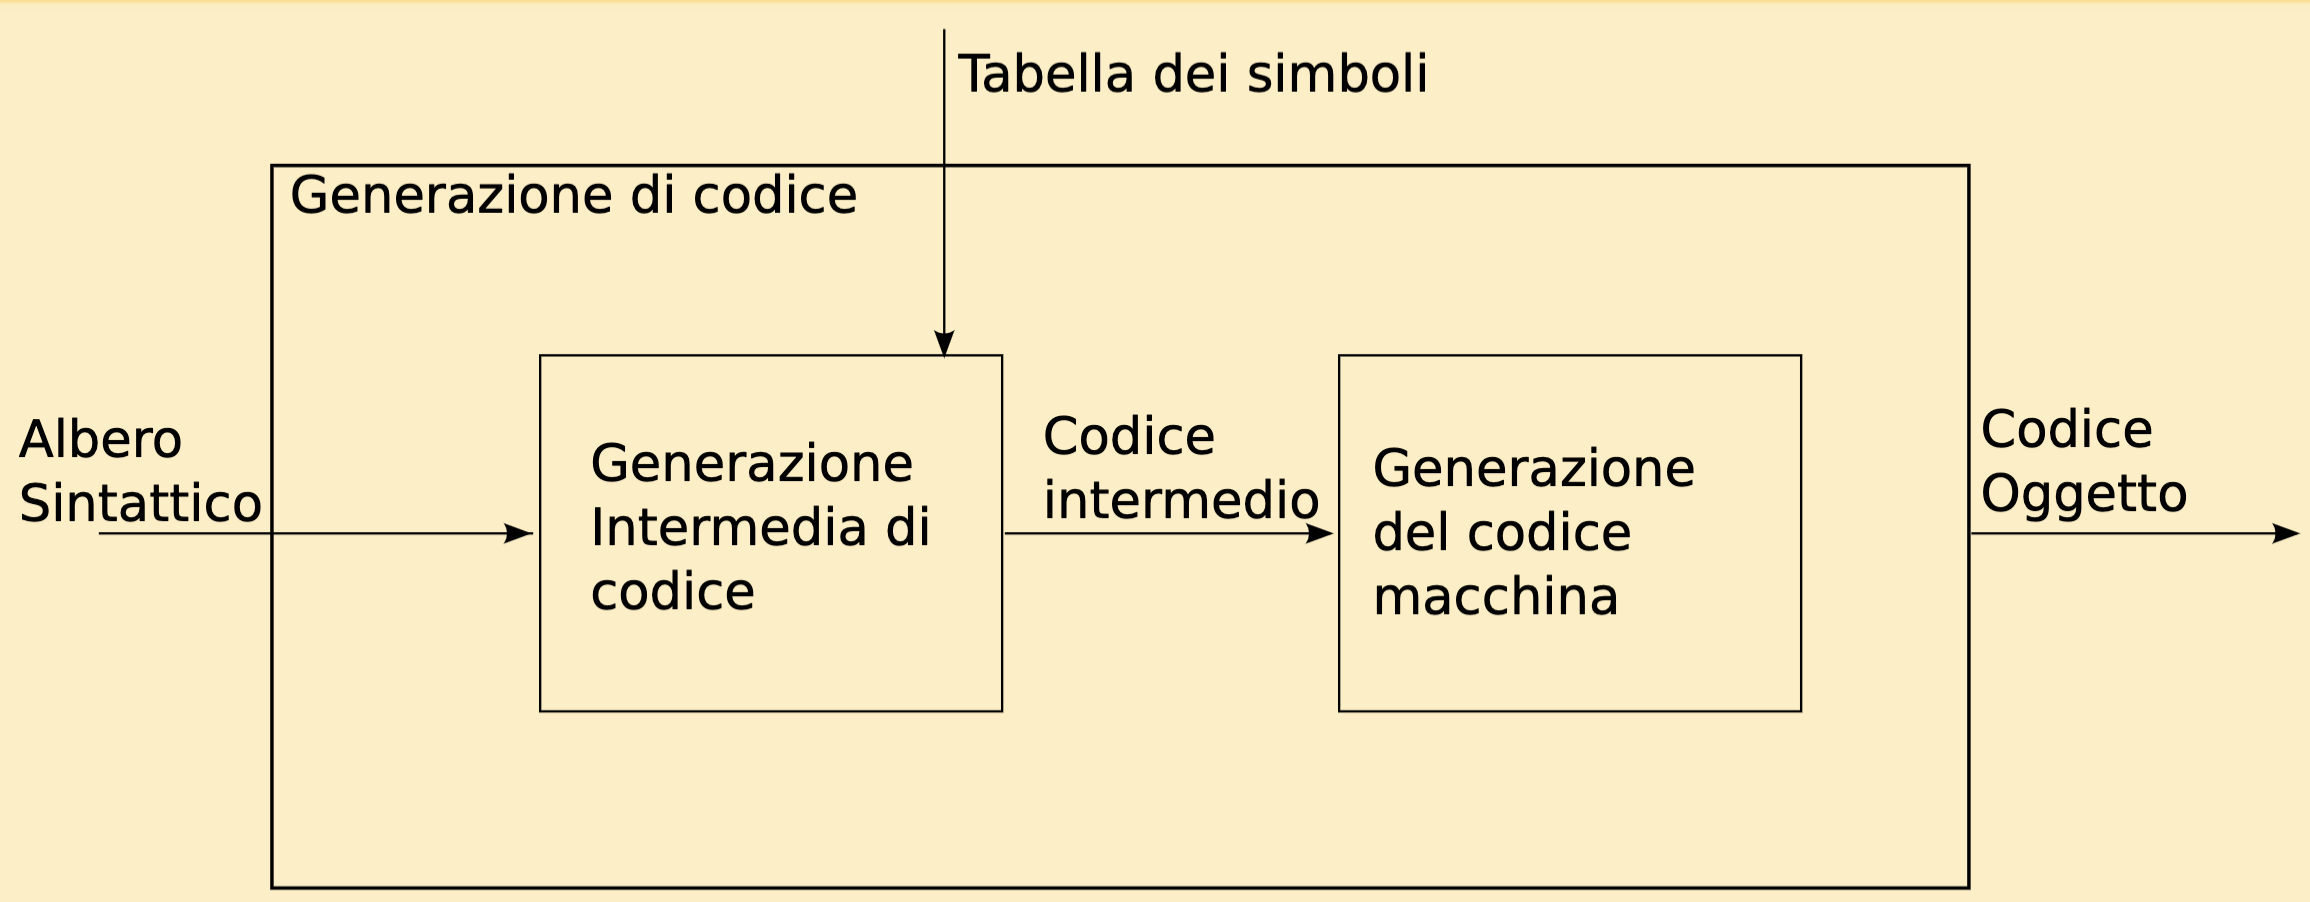
\includegraphics[width=1\linewidth]{assets/gencod.png}
    \caption{Ulteriore modularizzazione del modulo di generazione del codice}
\end{figure}

\newpage
\chapter{Processo di produzione software}

\paragraph{Code and Fix} Primo approccio a scatola nera, nato agli albori dell'informatica, in cui non esiste distinzione tra utente e programmatore.
Il modello di sviluppo (ciclico) seguito era molto semplice:
\begin{enumerate}
    \item \textit{Code}: fase di implementazione
    \item \textit{Fix}: fase di manutenzione
\end{enumerate}
Approccio fallimentare, faceva errato uso della \textit{duttilità} del software. Portò alla \textit{crisi dell'ingegneria del software} (anni '80), che (tra le altre) introdusse il \textit{problema del feedback}: riscontro tempestivo (da parte del committente) sul lavoro svolto (dal team di sviluppo).

\section{Obiettivi del processo}

Gli \textbf{\textit{obiettivi del processo}} di sviluppo sono:
\begin{enumerate}
    \item Standardizzazione
    \item Predicibilità
    \item Produttività
    \item Qualità del prodotto
\end{enumerate}

\paragraph{Modello di produzione (\textit{Boehm, 1988})} Basato su l'\textit{ordine degli stadi coinvolti} e \textit{criteri di transizione}: consentono di progredire dallo stadio corrente a quello successivo. Definisce relazioni ed ordine di esecuzione delle attività (le quali prevedono dei "prodotti intermedi" come output per la prossima fase).

\begin{figure}[ht!]
    \centering
    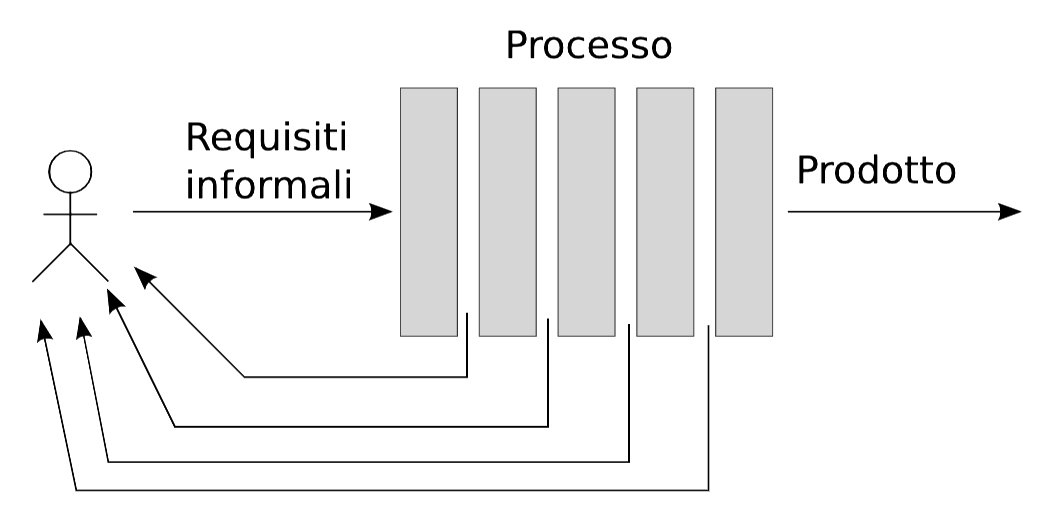
\includegraphics[width=0.8\linewidth]{assets/processo_esplicito.png}
    \caption{Se si segue un \textbf{modello esplicito} lo sviluppo software procede in modo ordinato e prevedibile (riduzione degli errori)}
\end{figure}

\begin{figure}[ht!]
    \centering
    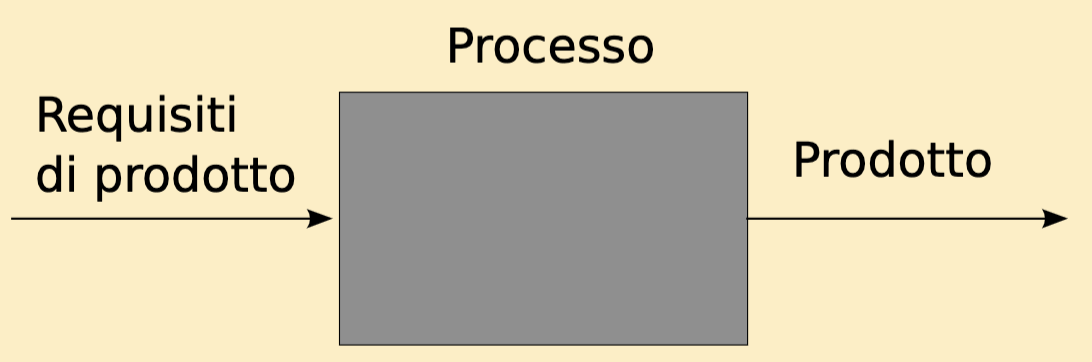
\includegraphics[width=0.8\linewidth]{assets/processo_blackbox.png}
    \caption{Se NON si segue un modello preciso lo sviluppo viene considerato una scatola nera (\textbf{black box}), in cui gli input sono i requisiti del prodotto e l'output il prodotto stesso.}
\end{figure}

\newpage

\section{Attività del processo di sviluppo}
Attività fondamentali del processo di produzione software. Devono essere eseguite a prescindere dal modello di sviluppo adottato. Ogni fase restituisce un \textit{artefatto} in output. Gli \textit{artefatti intermedi} (non rilasciati al cliente) contribuiscono al prodotto finale (sistema software).

\subsection{Studio di fattibilità}
Viene eseguito da personale qualificato, consiste in una simulazione del processo di sviluppo sotto vari scenari. Ha come output un documento che:
\begin{itemize}
    \item Definisce il problema
    \item Elenca soluzioni alternative (costi e benefici)
    \item Esplicita risorse richieste, costi e date di consegna
\end{itemize}
La \textit{\textbf{SWOT Analysis}} è uno strumento di pianificazione strategica per progetti che richiedono decisioni ad ogni raggiungimento di obiettivo. Distingue i seguenti elementi:
\begin{itemize}
    \item \textit{Strengths}: interne al progetto, utili.
    \item \textit{Weaknesses}: interne al progetto, di ostacolo.
    \item \textit{Opportunities}: esterne al progetto, vantaggiose.
    \item \textit{Threats}: esterne al progetto, di impedimento.
\end{itemize}

\subsection{Analisi e specifica dei requisiti}
Consiste nello:
\begin{itemize}
    \item stabilire se le richieste del cliente (\textit{requisiti}) siano soddisfacibili e con quale grado di qualità;
    \item formalizzare le richieste in una serie di \textit{features} che l'applicazione deve assicurare (in un \textit{documento di specifica})
    \item occuparsi dell'individuazione degli \textit{stakeholder} (persone, aziende, entità interessate al sisema)
\end{itemize}

\paragraph{Modularizzazione orizzontale} Consiste nell'analizzare il progetto sullo stesso piano di astrazione da diversi punti di vista (uno per ogni aspetto del problema), strutturando il sistema come collezione di viste come:
\begin{itemize}
    \item \textit{Modello dei dati} (Diagramma ER, Class diagram)
    \item \textit{Modello delle funzioni eseguibili} (Flux o Use Case diagram)
    \item \textit{Modello di controllo di esecuzione} (Reti di Petri, State diagram)
\end{itemize}

\paragraph{Classificazione dei requisiti}
\begin{itemize}
    \item \textbf{MUST}: relativi alla \textit{correttezza}, requisiti minimi per considerare il sistema accetabile;
    \item \textbf{SHOULD}: relativi alla \textit{robustezza}, requisiti desiderabili, ma la cui omissione non compromette le funzionalità di base;
    \item \textbf{MAY}: requisiti facoltativi, tralasciabili in caso di mancanza di risorse.
\end{itemize}

\paragraph{Documento di specifica} Output di questa fase, sottoposto agli stakeholder. Deve essere comprensibile, preciso, completo, consistente, non ambiguo e facile da modificare. Può contenere un piano di test del sistema e/o una versione preliminare del manuale utente. È strutturato come segue:
\begin{itemize}
    \item \textit{Dominio}: breve descrizione del dominio applicativo e obiettivi da raggiungere.
    \item \textit{Requisiti funzionali}: descrivono cosa dovrà fare il prodotto (formali).
    \item \textit{Requisiti non funzionali}
    \item \textit{Requisiti del processo di sviluppo e manutenzione}: procedure di controllo qualità, priorità di sviluppo tra, possibili cambiamenti del sistema.
\end{itemize}

\subsection{Definizione e progettazione dell'architettura software}
Produzione di un \textit{documento di specifica di progetto} che descrive la struttura del sistema in termini di \textit{componenti}, relative interfacce e relazioni fra essi (motivando ogni scelta). Può richiedere l'uso di notazioni standard (come \textit{UML}).

\subsection{Produzione di codice e test di moduli}
Il team di programmatori procede ad implementare e testare i singoli moduli (in maniera indipendente). L'output di questa fase è il codice sorgente dei moduli.

\subsection{Integrazione e test del sistema}
Fase di assemblaggio del sistema a partire dai singoli moduli (seguendo criteri \textit{top-down} o \textit{bottom-up}). Nel caso di modelli incrementali i moduli sono sviluppati, testati e integrati nel sistema man mano. L'applicazione completa viene sottoposta ad un primo test (\textbf{\textit{"Alpha test"}})

\subsection{Rilascio, installazione e manutenzione}
Il \textit{rilascio} avviene in due fasi:
\begin{itemize}
    \item Distribuzione ad un gruppo selezionato di clienti (\textbf{\textit{"Beta test"}})
    \item Rilascio ufficiale sul mercato (\textit{\textbf{"Release"}})
\end{itemize}
L'\textit{installazione} definisce l'architettura del sistema a tempo di esecuzione.
La \textit{manutenzione} ha inizio (fase più costosa, 60\% c.d.p.):
\begin{itemize}
    \item Adattiva, correttiva (20\% c.d.m.)
    \item Perfettiva (50\% c.d.p.)
\end{itemize}

\newpage
\begin{figure}[H]
    \centering
    \subfloat[Classico]{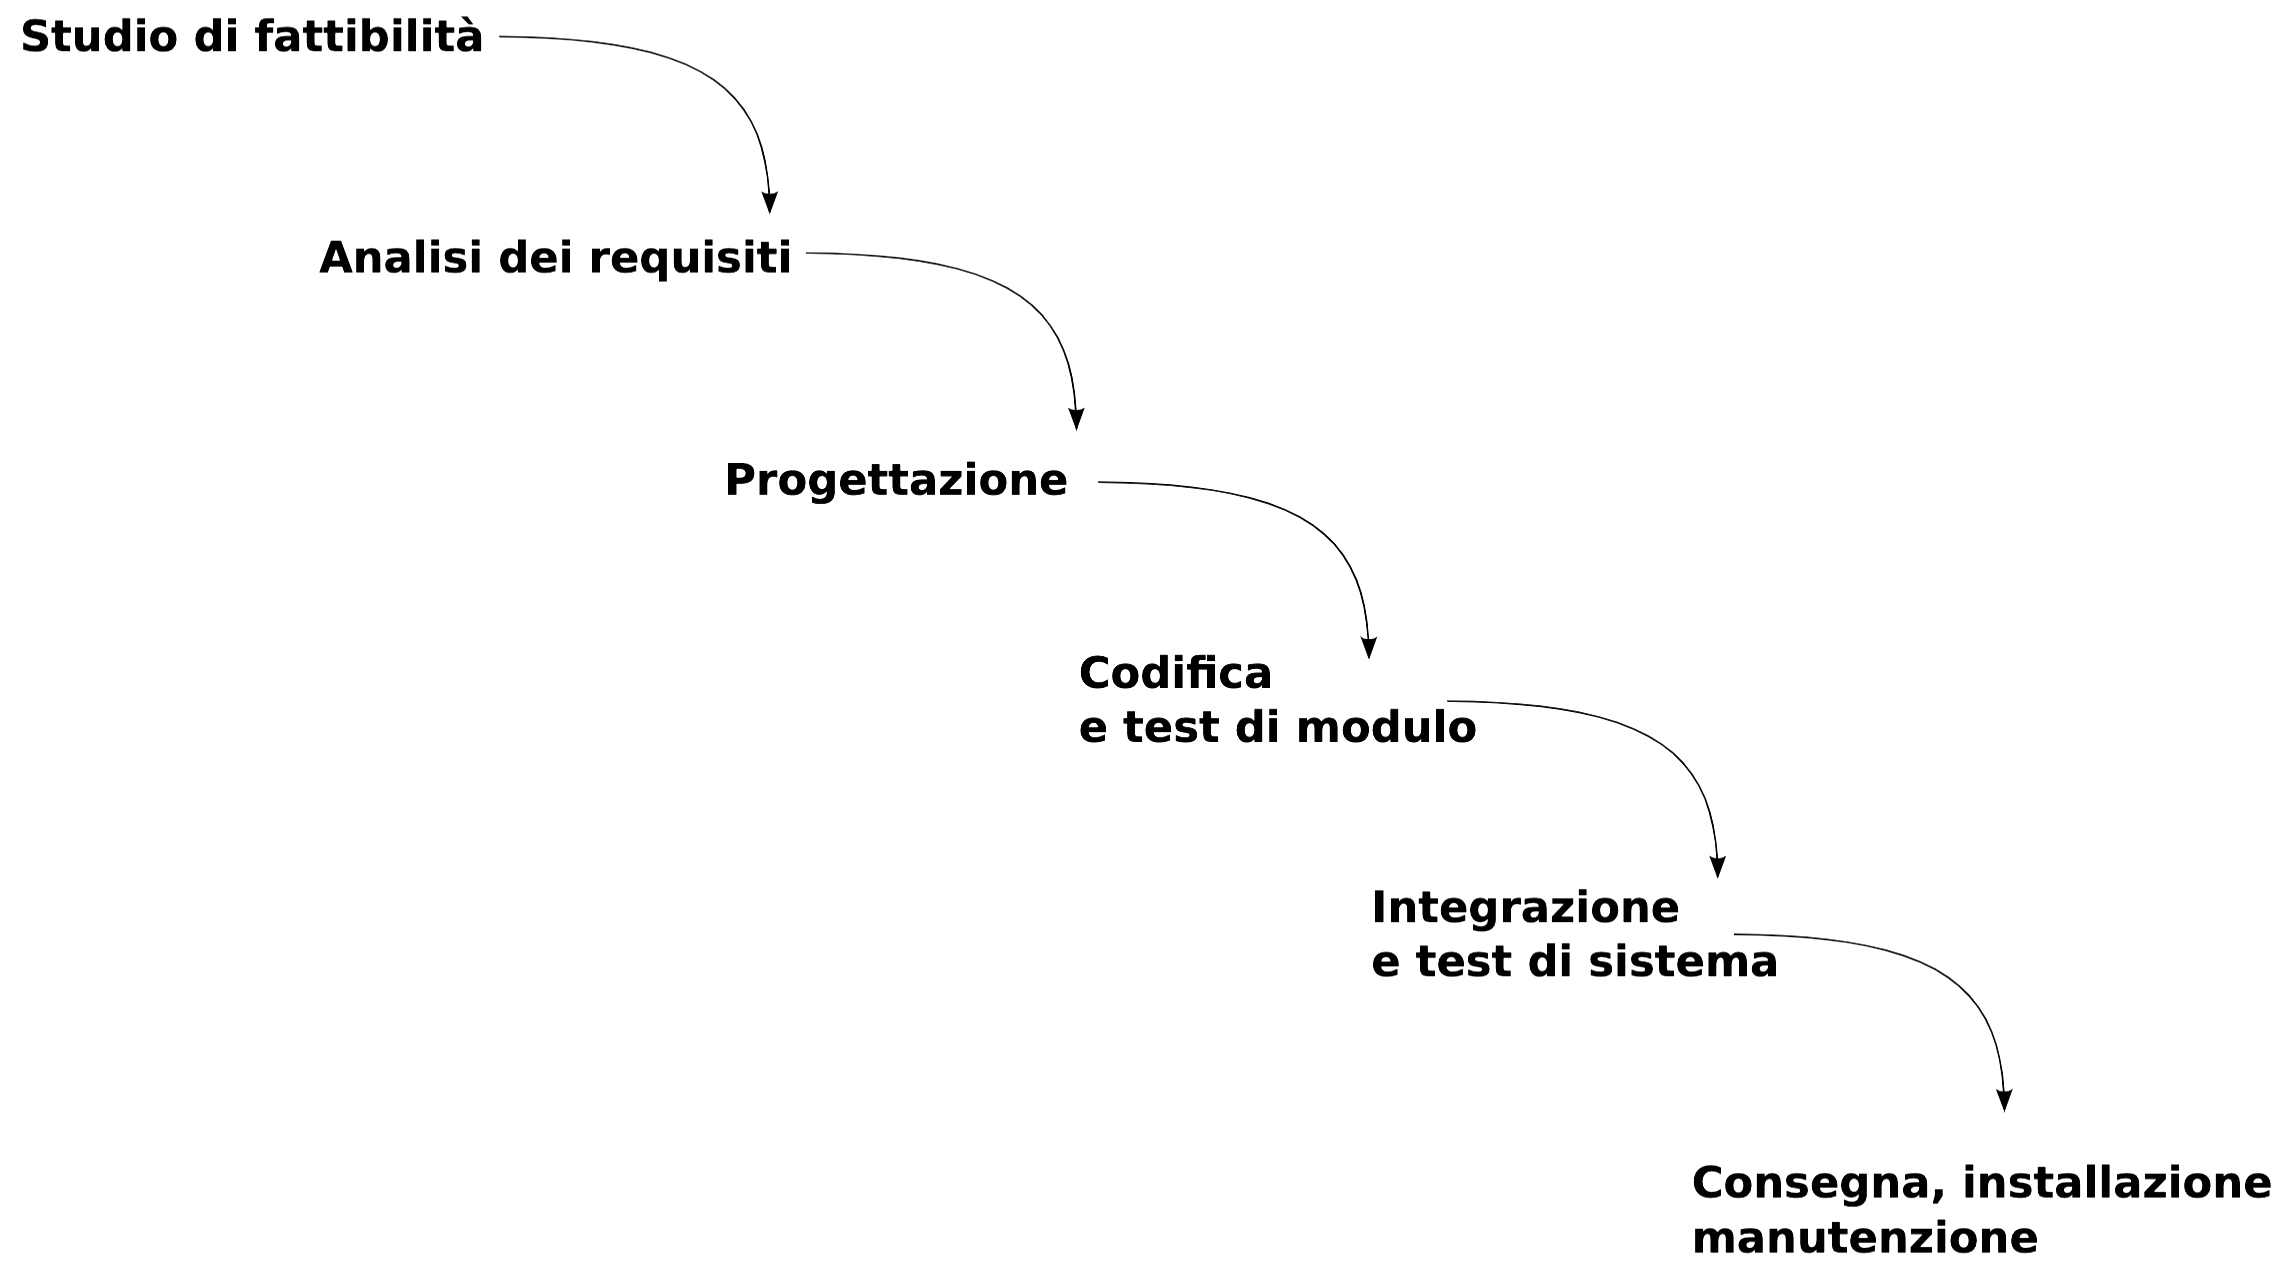
\includegraphics[width=0.48\textwidth]{assets/waterfall.png}\label{fig:waterfall}}
    \hfill
    \subfloat[Con feedback]{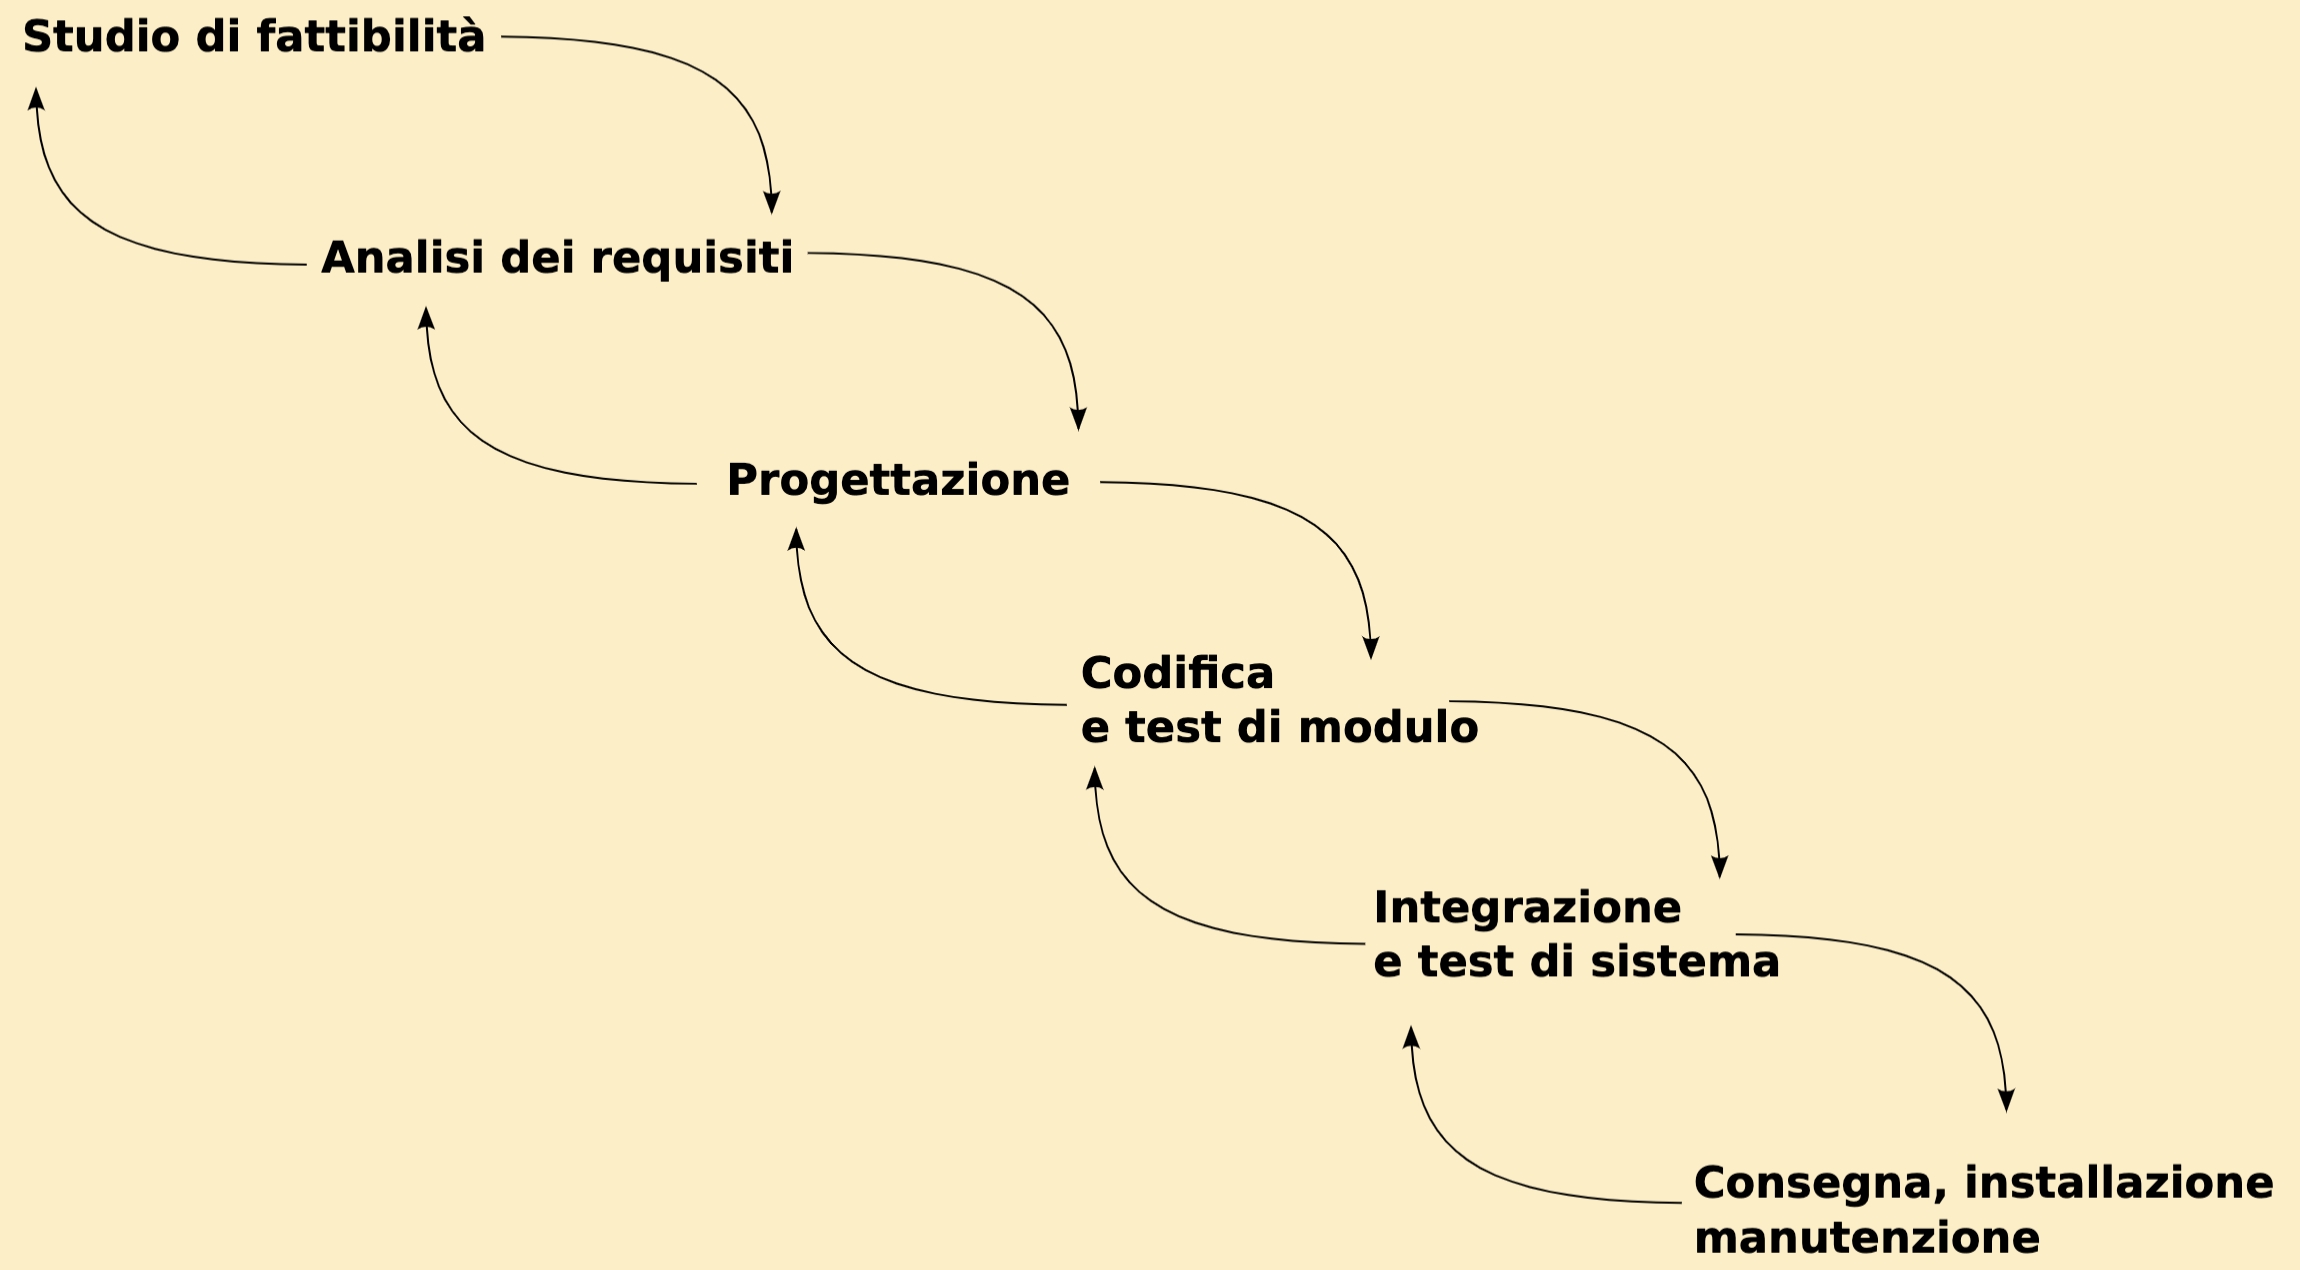
\includegraphics[width=0.48\textwidth]{assets/waterfall_fb.png}\label{fig:waterfall-fb}}
    \caption{Modelli a cascata}
\end{figure}

\chapter{Testing}

Il \textbf{testing} è un sottoinsieme di un ambito più generale: la \textbf{\textit{verifica}}.
Questa può essere \textit{soggettiva} o \textit{oggettiva}, e si può concentrare su qualità interne o esterne. Il risultato del processo di testing non è una risposta binaria (SÌ o NO), ma l'individuazione di difetti con diversi \textit{livelli di severità}.

Gli \textit{approcci alla verifica} sono di tipo:
\begin{itemize}
    \item \textbf{Dinamico} (testing): si valuta il comportamento del software in esecuzione;
    \item \textbf{Statico}: si analizzano le proprietà del prodotto software.
\end{itemize}

\paragraph{Testing} Consiste nell'ottenere \textbf{campioni di comportamento} sottoponendo il programma a particolari \textit{test-case}: configurazioni di input e casistiche. \textit{Manca di continuità} poiché non è definibile un test in grado di garantire che il comportamento del sistema sia corretto in ogni situazione. Idealmente un test dovrebbe essere \textbf{ripetibile}, ovvero presentare gli stessi risultati sotto le stesse condizioni, caratteristica influenzata da: ambiente esterno, task con esiti non deterministici (es. generazione di numeri pseudo-random).

\paragraph{Dijkstra (1987)} “L'obiettivo del testing è individuare la presenza di bug nel sistema ed isolarli attraverso l'applicazione di principi sistematici e metodi accurati, di modo da facilitarne la correzione” (\textit{debugging}).

\paragraph{Formalmente} Dati $D$ insieme dei possibili input ed $R$ insieme dei possibili output, un programma $P$ è definito come:
\begin{center}
    $P : D \rightarrow R$
\end{center}
Funzione \textbf{parziale} poiché potrebbero esistere elementi di $D$ non corrispondenti ad alcun elemento in $R$ (funzione non definita).

\paragraph{Nota} Il testing del software è afflitto dal \textbf{problema dell'oracolo} (entità responsabile di esaminare i risultati dei test, stabilendo se siano accettabili o meno). Spesso far valutare ogni risultato da un operatore umano risulta essere lento e inefficiente: è necessario “automatizzare” l'oracolo. La progettazione di un oracolo automatico è un processo complesso e privo di una soluzione universalmente valida:
\begin{itemize}
    \item lo sviluppo D-by-C favorisce l'analisi automatica del testing; 
    \item la presenza di specifiche informali o di molti fattori esterni rende spesso necessario un oracolo umano.
\end{itemize}
Inoltre, il testing non dovrebbe limitarsi a verificare le funzionalità di un sistema software, ma dovrebbe anche affrontare:
\begin{itemize}
\item \textit{Overload}: risposta del sistema a carichi di lavoro eccessivi;
\item Robustezza e regressione del sistema;
\item Concorrenza (che introduce effetti non deterministici);
\item Diverse configurazioni temporali (solo nei sistemi real time);
\end{itemize}

\section{Correttezza}

La correttezza del programma è descritta dal sottoinsieme:
\begin{center}
$O \subseteq D \times R$    
\end{center}
Preso $d \in D$, un \textbf{output $P(d)$ è corretto} se la coppia $\langle d, P(d) \rangle$ è ammissibile (appartiene a $O$). Un \textbf{programma $P$ è corretto} se ogni suo output è corretto (verificabile solo per $D$ finito). Un output si dice \textbf{fallimento} se è errato per l'input $d$ o se $P(d)$ non è definito. Un \textbf{errore} è la causa di un fallimento, al suo verificarsi il programma entra in uno stato intermedio incorretto: \textbf{fault}.

\paragraph{Test Case} Definito come $t \in D$, ha successo SSE $P(t)$ è corretto.

\paragraph{Test Set} Definito come $T \subseteq D$, ha successo SSE $P(t)$ è corretto $\forall t \in T$. Nel caso in cui il programma $P$ sia scorretto, un test set si dice \textbf{ideale} se $\exists t \in T$ t.c. $P(t)$ non è corretto (ovvero, \textit{esiste un test set all'interno del test case che trova l'errore}).

\section{Criteri di testing}

Un \textbf{criterio} è una regola per definire dei sottoinsiemi finiti di $D$ (test set).
Sia $2^D$ l'insieme di tutti i possibili sottoinsiemi di $D$, $C$ è un insieme tale che:
\begin{center}
    $C \subseteq 2^D$ (finito)
\end{center}
Un \textbf{test set $T$ soddisfa} un criterio $C$ se:
\begin{center}
    $T \in C$    
\end{center}

\paragraph{Esempio} Sia $D$ il dominio dei numeri interi, definiamo il seguente criterio:
\begin{center}
    $C = \{x_1, x_2, ..., x_n\} \mid n \ge 3 \land \exists i, j, k \mid x_i < 0, x_j = 0, x_k > 0$    
\end{center}
Il criterio richiede un test set tale per cui esistano almeno 3 numeri interi: uno positivo, uno negativo ed uno pari a zero.
\begin{center}
    $T_1 = \{-5, 0, 12\}$ soddisfa $C$    
\end{center}
\begin{center}
    $T_2 = \{9, 0, 18\}$ NON soddisfa $C$    
\end{center}

\subsection{Proprietà}

\paragraph{Consistenza} Dato un criterio $C$, comunque si prendano $T_1, T_2 \in C$, $T_1$ ha successo SSE anche $T_2$ ha successo. Ergo: tutti i test set che soddisfano $C$ sono equivalenti e danno lo stesso risultato.

\paragraph{Completezza} Un criterio $C$ è detto \textbf{completo} se, posto il programma $P$ non corretto, esiste almeno un test set $T \in C$ che non ha successo.

Nella pratica non è possibile definire un algoritmo che stabilisca se un criterio sia consistente e completo. Ciò non significa che i test set possano essere scelti senza criterio ed in modo casuale (sarebbe inadeguato).

\paragraph{Finezza} Un criterio $C_1$ si dice \textbf{più fine} di un criterio $C_2$ se investiga più casi, deve valere che:
\begin{center}
    $\forall P, \forall T$ che soddisfa $C_1$, $\exists T^I \subset T$, con $T^I \in C_2$
\end{center}
Il testing, guidato dall'\textit{esperienza empirica}, è mirato alla definizione di \textbf{test set significativi} che hanno buone probabilità di rilevare la presenza di errori.

\paragraph{Criterio della copertura completa} Criterio empirico che prevede due fasi. Nella prima fase si divide il dominio $D$ in una serie di \textit{sottodomini} $D_i$
\begin{center}
    $\{D_1, D_2, \ldots, D_n\}\ |\ D = D_1 \cup D_2 \cup \ldots \cup D_n$
\end{center}
che rispettano le proprietà: riflessiva, simmetrica e transitiva.
Se i sottodomini sono \textit{disgiunti} ($D_i \cap D_j = \emptyset$) si dice che costituiscono una \textbf{partizione} di $D$. In una seconda fase si crea un test set selezionando un elemento per ogni sottodominio $D_i$, se non formano una partizione si possono scegliere gli elementi in comune per \textit{minimizzare} la dimensione del test set.

I criteri di testing partizionano il dominio di input $D$ in \textbf{classi di equivalenza}, la maggior parte degli errori in un software tende a concentrarsi nelle “\textit{zone di confine}” fra le classi. Un test set dovrebbe prediligere le condizioni di confine (\textit{boundary}) rispetto alle condizioni interne.

\newpage

\section{Strategie di testing}

Il testing di componenti software può seguire due strategie complementari (idealmente andrebbero applicate entrambe).

\subsection{White Box - Strutturale}

Il criterio di partizione per derivare il test set si basa sul codice del componente (trasparente, visibile), deve testare ogni parte significativa del codice ("copertura strutturale"), altrimenti è inadeguato, e si concentra sul flusso di controllo del codice verificando esattamente ciò che il componente fa.

\subsubsection{Tipologie}

\paragraph{Statement Coverage} Si seleziona un test set tale da far eseguire almeno una volta ogni istruzione elementare del componente. Il limite del criterio è che provare ogni istruzione del codice non significa assicurarsi di esplorare ogni possibile flusso di esecuzione.
   
\paragraph{Edge Coverage} Si seleziona un test set tale da esplorare almeno una volta ogni possibile flusso di esecuzione del componente. Richiede la costruzione preliminare del “grafo di controllo” del codice: 
\begin{itemize}
       \item gli archi (orientati) rappresentano un'istruzione; 
       \item il nodo d'uscita dell'arco è la condizione di partenza dell'istruzione;
       \item il nodo d'ingresso è la condizione d'arrivo dell'istruzione. 
\end{itemize}
Il criterio prevede che ogni ramo del grafo di controllo del codice sia preso in considerazione almeno una volta. Il limite del criterio è che, pur esplorando ogni ramo del flusso, non coglie i differenti motivi che possono portare a seguire un ramo se la condizione d'ingresso è composta.
   
\paragraph{Condition Coverage} Si seleziona un test set tale da esplorare almeno una volta ogni possibile flusso di esecuzione del componente e di valutare in maniera indipendente almeno una volta ogni valore costituente di condizioni composte. Il limite del criterio è che alle volte non basta ispezionare ogni istruzione del codice e tutti i flussi di controllo per rilevare l'errore: alcune istruzioni possono comportare errore per determinati input e non per altri.
   
\paragraph{Path Coverage} Si seleziona un test set tale da esplorare tutti i possibili percorsi dal nodo iniziale al nodo finale del grafo di controllo. Il limite è che il numero di percorsi potrebbe essere troppo elevato o addirittura infinito (cicli), rendendo il criterio inapplicabile (\textit{path explosion}).

\begin{figure}[H]
    \centering
    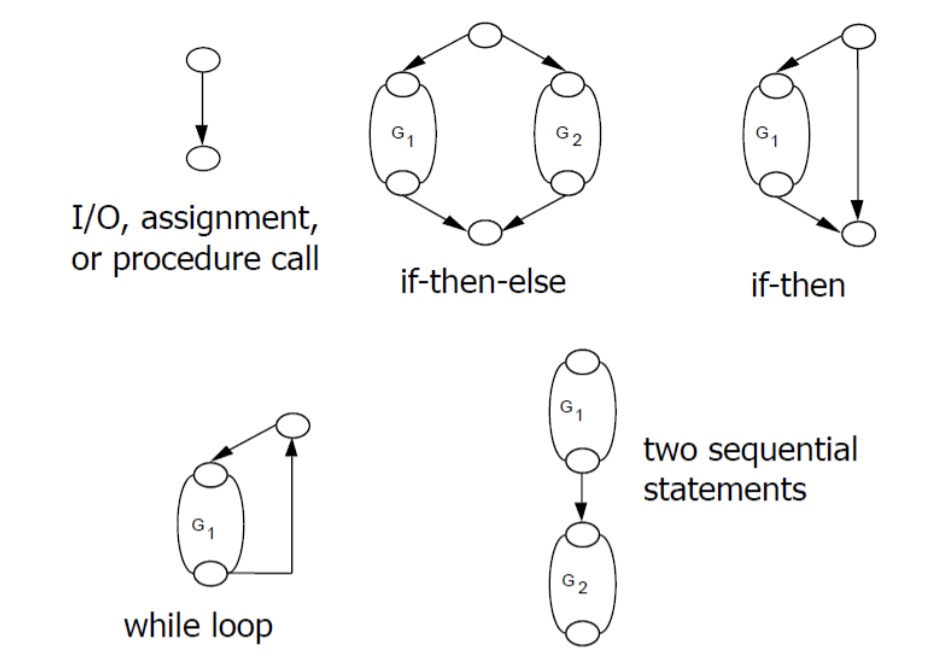
\includegraphics[width=0.75\linewidth]{assets/wb-control-graph.png}
    \caption{Regole di costruzione del grafo di controllo}
    \label{fig:wb-graph}
\end{figure}

\subsubsection{Limiti}
Potrebbe essere infattibile coprire l'intera struttura del codice, riducendo la percentuale di adeguatezza del test. Inoltre, il personale adibito ai test deve avere una buona conoscenza del programma e il test dipende strettamente dall'implementazione:
\begin{itemize}
    \item se l'implementazione cambia è necessario modificare anche il test; 
    \item tutti gli elementi della specifica che non sono esplicitamente implementati nel codice vengono ignorati. 
\end{itemize}

\subsection{Black Box - Funzionale}

Il criterio di partizione per derivare il test set si basa sulla specifica del componente, astraendo dal codice. Si verifica ciò che il componente si propone di fare. È riusabile per più programmi perché non dipende dall'implementazione ma si basa sulla specifica del modulo. Si cerca di derivare un test set significativo a partire dalla specifica del componente, cercando di:
\begin{itemize}
    \item coprire tutte le possibili situazioni di funzionamento;
    \item trovare dei \textit{controesempi} (situazioni in cui il componente potrebbe non funzionare). 
\end{itemize}

\subsubsection{Tipologie}

\paragraph{Testing derivato da pre-condizioni e post-condizioni logiche del componente} Adatto a componenti DBC.

\paragraph{Testing derivato dal linguaggio degli input attesi dal programma} Si cerca di avere una copertura totale della sintassi (ogni regola grammaticale deve essere esercitata almeno una volta). È indicato per testare sistemi software come compilatori o interpreti. Essendo la sintassi di un linguaggio un oggetto formale, i test set si prestano ad essere generati automaticamente.

\paragraph{Testing basato su tabella delle decisioni} Rappresentazione tabulare dei possibili input in relazione alle diverse condizioni in cui il sistema può trovarsi, la cella indica:
\begin{itemize}
    \item ($true$) determina - condizione soddisfatta;
    \item ($false$) non determina - condizione non soddisfatta;
\end{itemize}
La tabella mostra tutte le possibili combinazioni di input, aiutando i progettisti a derivare sistematicamente un test set.

\paragraph{Testing basato su grafi causa-effetto} Rappresenta i diversi effetti di possibili combinazioni di input, da cui derivare sistematicamente il test set. Nel grafo sono presenti dei nodi:
\begin{itemize}
    \item AND (due o più combinazioni si verificano contemporaneamente);
    \item OR (si verifica almeno una di due o più combinazioni).
\end{itemize}
Il criterio di copertura prevede di testare tutte le possibili combinazioni di input, il numero di combinazioni da testare si può ridurre partendo dagli output e procedendo a ritroso:
\begin{itemize}
    \item se si incontra un nodo OR con output $true$ è sufficiente che solo una delle combinazioni in ingresso sia $true$;
    \item se si incontra un nodo AND con output $false$ è sufficiente che solo una delle combinazioni in ingresso sia $false$.
\end{itemize}

\newpage

\section{Fasi di testing}

\subsection{Test dei singoli moduli}

La difficoltà risiede nelle possibili dipendenze da altri moduli, si deve ricorrere a delle componenti software che “simulano” gli elementi con cui il modulo si troverà ad interagire:
\begin{itemize}
    \item \textbf{driver}: modulo che attiva il modulo testato; 
    \item \textbf{stub}: modulo che viene usato dal modulo testato;
\end{itemize}

\begin{figure}[H]
    \centering
    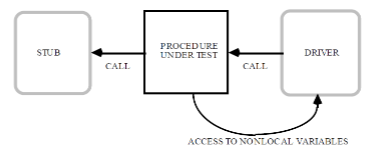
\includegraphics[width=0.75\linewidth]{assets/driver-stub.png}
    \caption{Driver e stub per il test dei moduli}
    \label{fig:driver-stub}
\end{figure}

\subsection{Test di integrazione}
Si testano insiemi di moduli, ottenuti secondo due strategie.

\paragraph{Big Bang} L'insieme si ottiene (e viene testato) solo dopo aver sviluppato e testato singolarmente ogni modulo.

\paragraph{Incrementale} Non appena un modulo viene sviluppato e testato, lo si integra nell'insieme e si procede al test complessivo tramite approccio:
\begin{itemize}
    \item \textbf{bottom-up}: si usano \textit{driver};
    \item \textbf{top-down}: si usano \textit{stub}.
\end{itemize}

\subsection{Test di sistema} Si testa il sistema complessivo (\textbf{\textit{Alpha Test}}).

\subsection{Test di accettazione} Valutazione da parte dei clienti di una versione rilasciata del sistema (\textbf{\textit{Beta Test}}).

\newpage

\paragraph{Testing con POO}

La \textit{Programmazione Orientata agli Oggetti} introduce nuovi aspetti (ereditarietà, polimorfismo, dynamic binding) di cui tenere conto nel testing. Una gerarchia di classi può essere testata tramite due strategie.

\paragraph{Appiattimento}  Si considera ogni classe concreta totalmente indipendente dalle altre.

\paragraph{Strategie ad-hoc} Traggono vantaggio dalla struttura gerarchica:
\begin{itemize}
    \item usare test che non devono essere ripetuti per ogni erede;
    \item usare test che devono essere eseguiti per una classe e tutti i successivi eredi;
    \item ripetere test con gli stessi input, verificando solo se l'output sia cambiato o meno;
    \item ripetere test aggiungendo parametri all'input e verificando che l'output cambi di conseguenza; 
\end{itemize}

\newpage

\chapter{Unified Modeling Language}

Per \textit{Unified Modeling Language} (UML) si intende una famiglia di notazioni grafiche atte a supportare la descrizione e il progetto di sistemi software (POO in particolare). Si tratta di uno standard relativamente aperto, nato dalla fusione di alcuni linguaggi grafici e di modellazione diffusi negli anni '80-'90. È stato riconosciuto dal \textit{Object Management Group} nel 1997, e nuove versioni sono state rilasciate fino al 2017, sebbene l'ultimo aggiornamento più consistente (UML 2.0) risalga al 2005 (anno in cui venne riconosciuto standard ISO).

\section{Prospettive}

Vengono distinte due prospettive di utilizzo.

\paragraph{Prospettiva software} Modellazione della struttura e del funzionamento del sistema (associazione elemento $\Leftrightarrow$ componente del programma).

\paragraph{Prospettiva concettuale} Modellazione del dominio d'interesse in cui il sistema agisce (associazione elemento $\Leftrightarrow$ concetto del contesto applicativo).
\\
\\
Analogamente, i diagrammi possono offrire due diverse prospettive sul sistema.

\paragraph{Vista statica} Studia i legami tra componenti software che sussistono a tempo di compilazione (dipendono da definizione e struttura del sistema) e non cambiano a \textit{runtime}.

\paragraph{Vista dinamica} Studia i legami tra componenti software che non esistono a tempo di compilazione, bensì nascono ed evolvono a \textit{runtime} (dipendono dal funzionamento del sistema).

\section{Utilizzo nel processo di sviluppo}

\paragraph{Analisi dei requisiti} Si fa uso di modelli informali (comprensibili a cliente/committente) per modellare gli aspetti più importanti del progetto e le interazioni fra sistema ed entità del contesto applicativo. Si adottano prospettive concettuale e software. È possibile abbozzare per la costruzione (\textit{forward engineering}) o la comprensione (\textit{reverse engineering}) di un sistema.

\paragraph{Progettazione} Si esprimono le decisioni progettuali in maniera dettagliata così da fornire ai programmatori un modello (spesso di interfaccia) da implementare. Si segue la prospettiva software, si possono produrre tramite strumenti di \textit{CASE} (o \textit{Computer Aided Software Engineering}). 

\paragraph{Codifica} A seconda del grado di progettazione, la programmazione diviene un'attività più o meno meccanica. Nel caso in cui sia massimo, il software si riduce a mera "traduzione diretta" dei modelli di progetto (alcuni CASE prevedono generazione automatica di codice).

\paragraph{Produzione di documentazione} Modelli concettuali o software possono essere impiegati per fornire una rappresentazione generale del sistema, descrivere gli scenari di funzionamento, evidenziare le caratteristiche e le relazioni più importanti di ogni componente (più o meno complesso).

\section{Diagrammi}

Lo standard UML (dalla versione 2.0) si basa su tre diagrammi ufficiali, per ognuno di essi sono stati definiti degli elementi tipici, pur lasciando la sintassi informale (si possono usare elementi appartenenti ad un diagramma in un altro). Tutti i diagrammi consentono l'inserimento di \textit{note} che permettono di specificare struttura, funzionamento o scopo di alcuni elementi. La notazione più diffusa prevede che sia scritta all'interno di un \textit{box-cartella} collegato da una linea tratteggiata all'elemento annotato.

\subsection{Activity}

L'\textbf{Activity Diagram} serve a descrivere logica procedurale, processi di business e workflow. In UML 1.0 era un caso particolare degli \textit{State Diagram}. Sono simili ai \textit{flowchart} ma supportano la rappresentazione di elaborazione parallela.

\paragraph{Descrizione} L'esecuzione inizia in corrispondenza del \textbf{nodo iniziale} (pallino nero) e si conclude al \textbf{nodo finale} (pallino bianco). I \textbf{nodi attività} (rettangolo a bordi smussati) descrivono le azioni da svolgere. I nodi sono collegati da \textbf{archi}; un percorso dal nodo iniziale al nodo finale rappresenta un \textbf{flusso di attività} (\textit{activity flow}). Per semplicità è possibile usare coppie di \textbf{connettori} con la stessa \textit{etichetta} al posto degli archi. I flussi possono essere:
\begin{itemize}
    \item \textbf{alternativi}: rombi con un solo arco entrante e più archi uscenti (\textbf{decision}) aventi ciascuno un proprio valore di \textit{guardia} (che ne decide l'esecuzione). I flussi confluiscono in un rombo con molti archi entranti ed un solo arco uscente (\textbf{merge}).
    \item \textbf{paralleli}: si diramano da una barra con un solo arco entrante e più archi uscenti (\textbf{fork}). I flussi possono essere eseguiti in maniera concorrente e confluiscono in una barra avente molti archi entranti ed un arco uscente (\textbf{join}).
\end{itemize}
All'interno di un nodo attività si può inserire un'icona a forma di rastrello che indica che l'attività è un flusso specificato da un ulteriore activity diagram di livello inferiore (diagramma secondario).

\begin{figure}[H]
    \subfloat[Semplice diagramma di esempio]{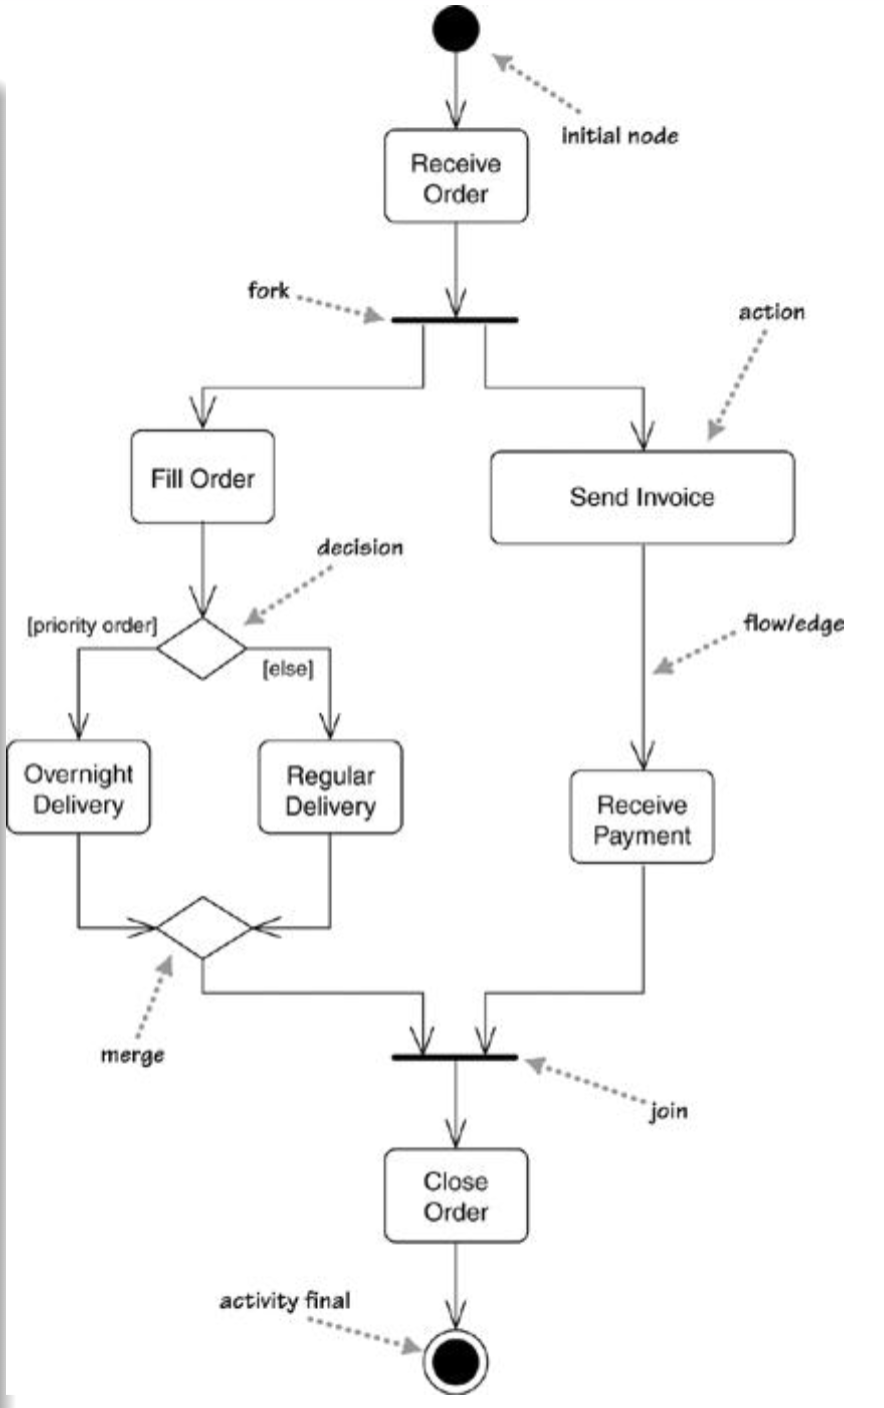
\includegraphics[width=0.4\linewidth]{assets/UML/activity/activity-1.png}}
    \hfill
    \subfloat[Esempio di partizione]{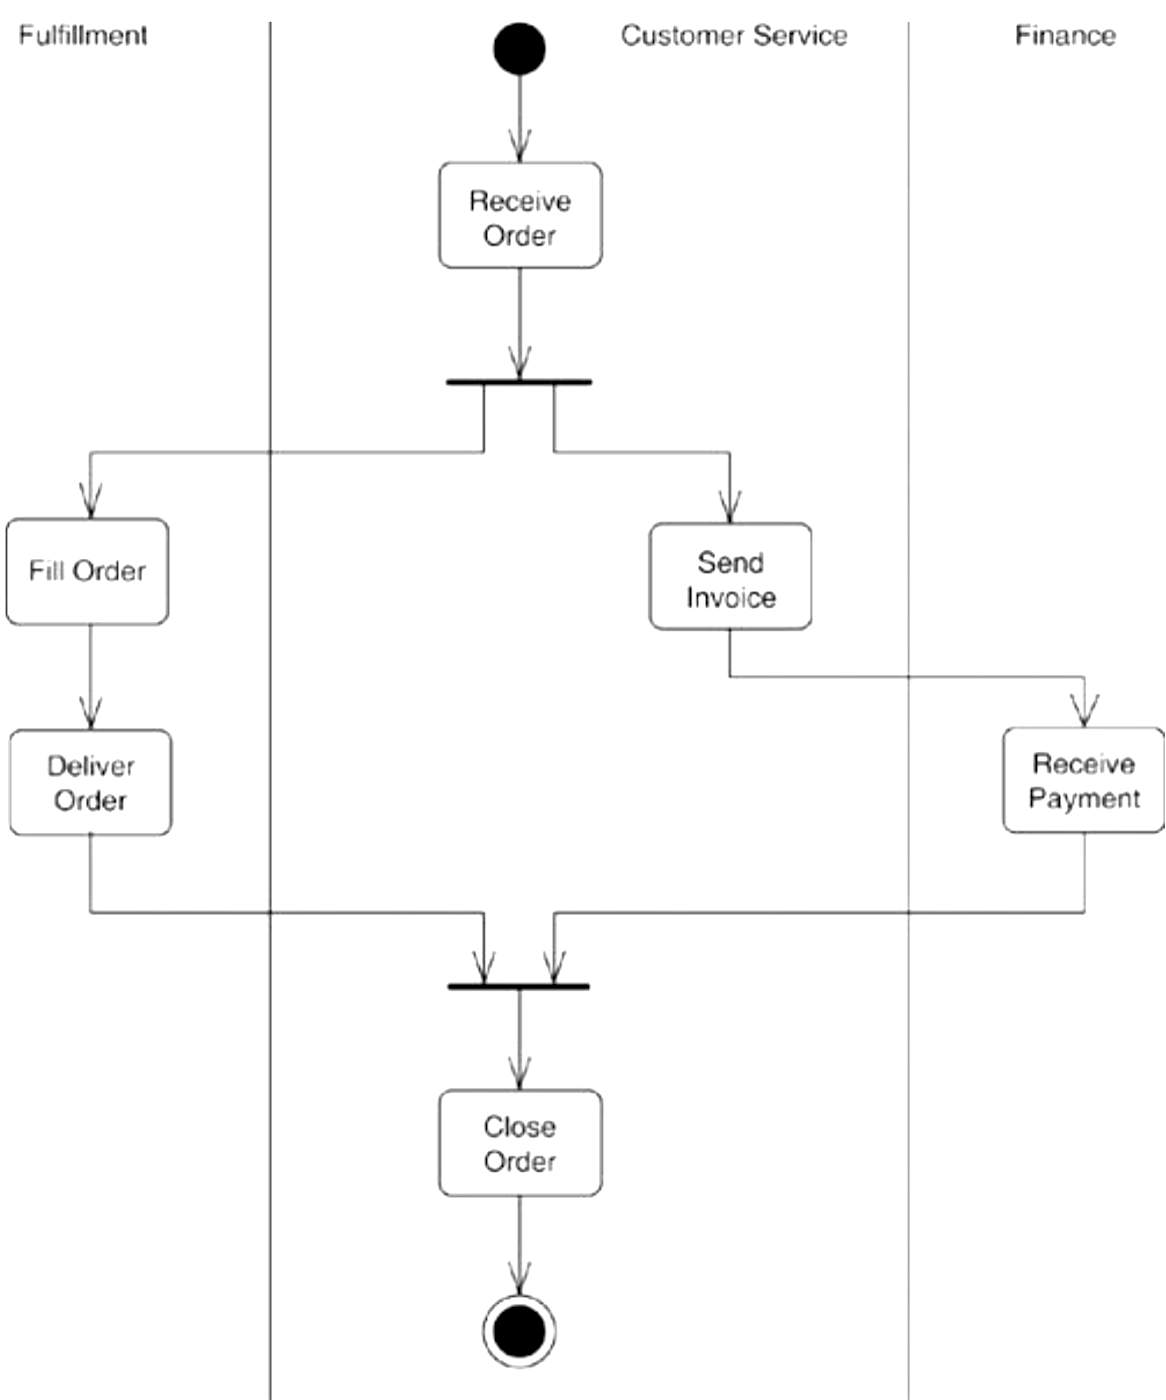
\includegraphics[width=0.55\linewidth]{assets/UML/activity/activity-3.png}}
\end{figure}

\paragraph{Specifiche di Join} Le operazioni di join operano la “sincronizzazione” tra flussi. È possibile introdurre una condizione booleana per la quale si può proseguire (viene rispettata) solo se tutti i flussi paralleli hanno terminato la loro esecuzione.

\paragraph{Partizioni} L'activity diagram può essere partizionato sulla base delle \textit{tipologie di attività} o dell'\textit{entità} adibita a svolgerle. Sono rappresentate tramite un'icona a \textit{rastrello}. Una determinata azione può essere implementata da un metodo; in tal caso si usa la sintassi “nomeClasse::nomeMetodo”. In un diagramma partizionato sono presenti delle \textbf{swim lane}: linee verticali che consentono di separare le competenze.

\begin{figure}[H]
    \subfloat[Diagramma secondario]{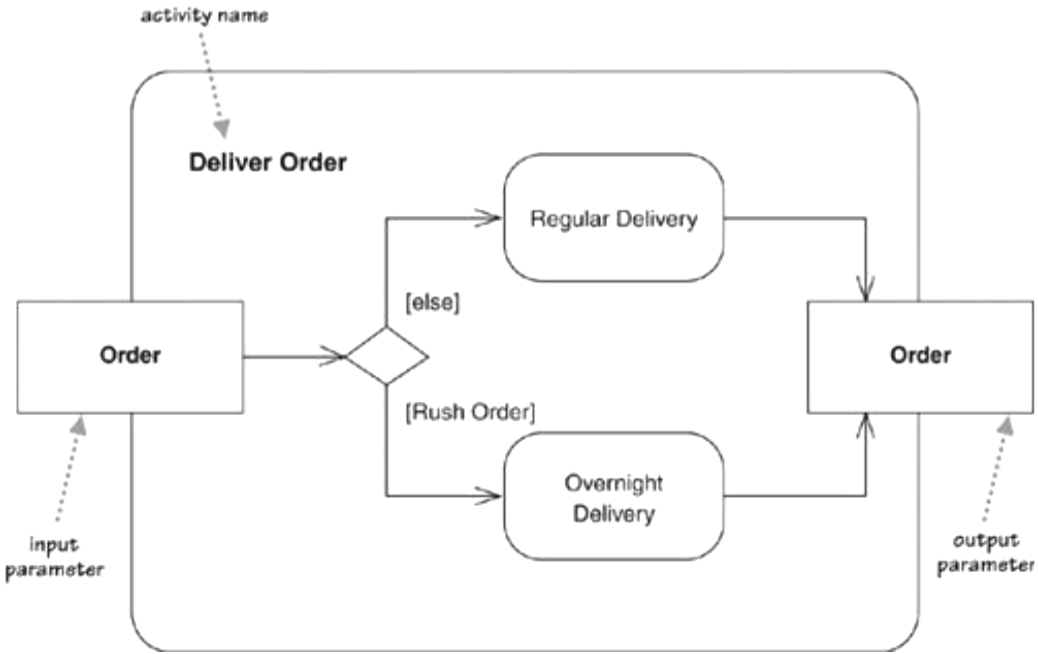
\includegraphics[width=0.55\linewidth]{assets/UML/activity/activity-2.png}}
    \hfill
    \subfloat[Utilizzo di flussi e connettori]{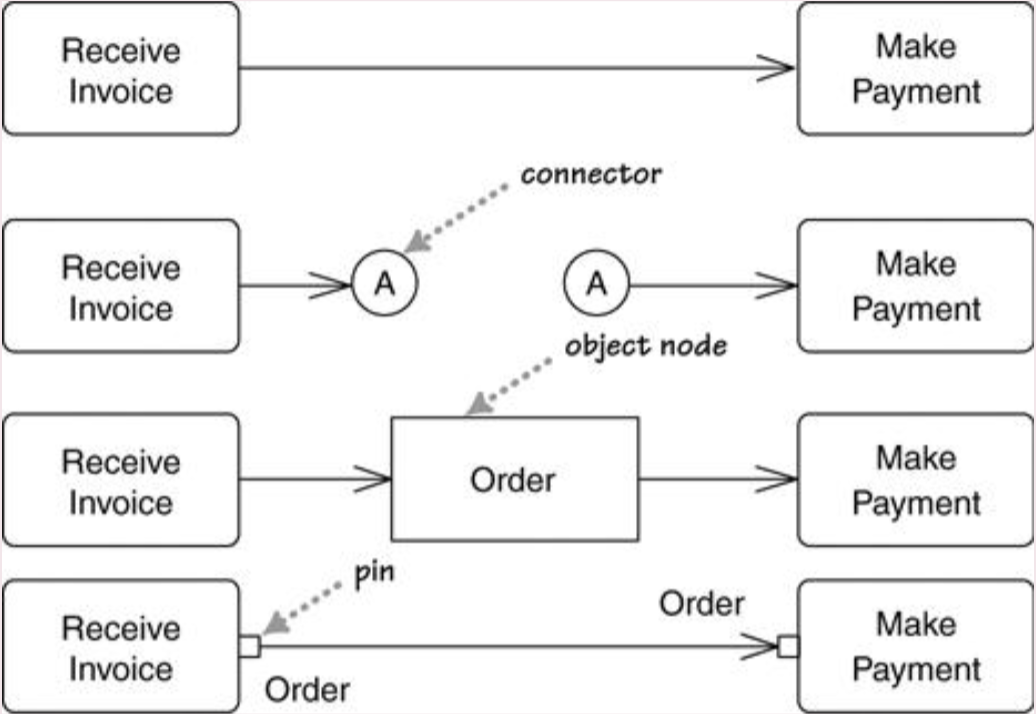
\includegraphics[width=0.4\linewidth]{assets/UML/activity/activity-4.png}}
\end{figure}

\newpage
\paragraph{Segnali} Eventi che il sistema può ricevere o generare da/verso l'esterno. Possono essere \textbf{temporali} (clessidre) o \textbf{personali} (generati da azioni, ad esempio).

\begin{figure}[H]
    \subfloat{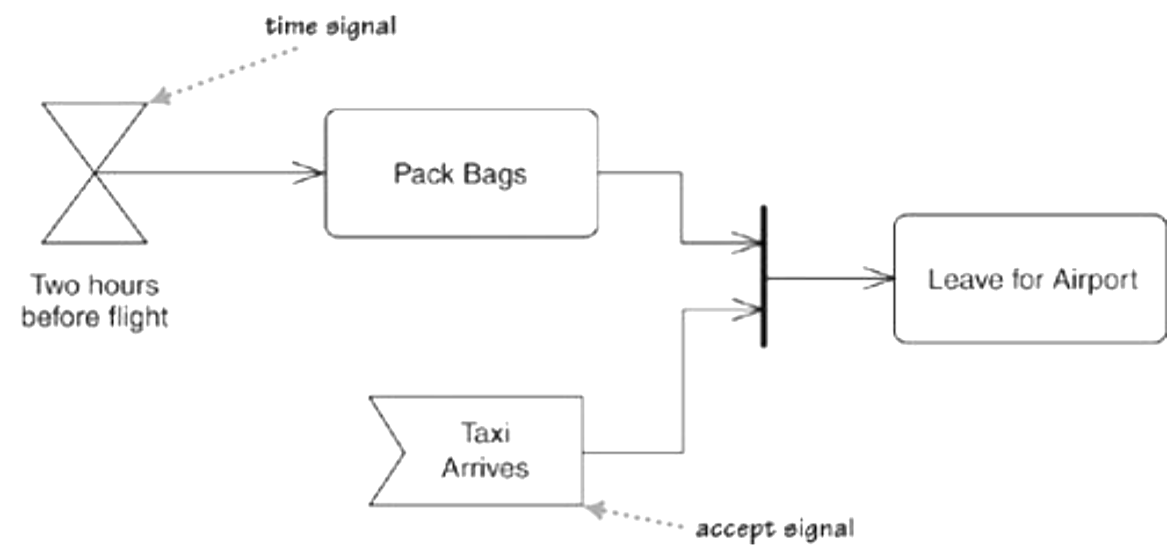
\includegraphics[width=0.455\linewidth]{assets/UML/activity/activity-6.png}}
    \hfill
    \subfloat{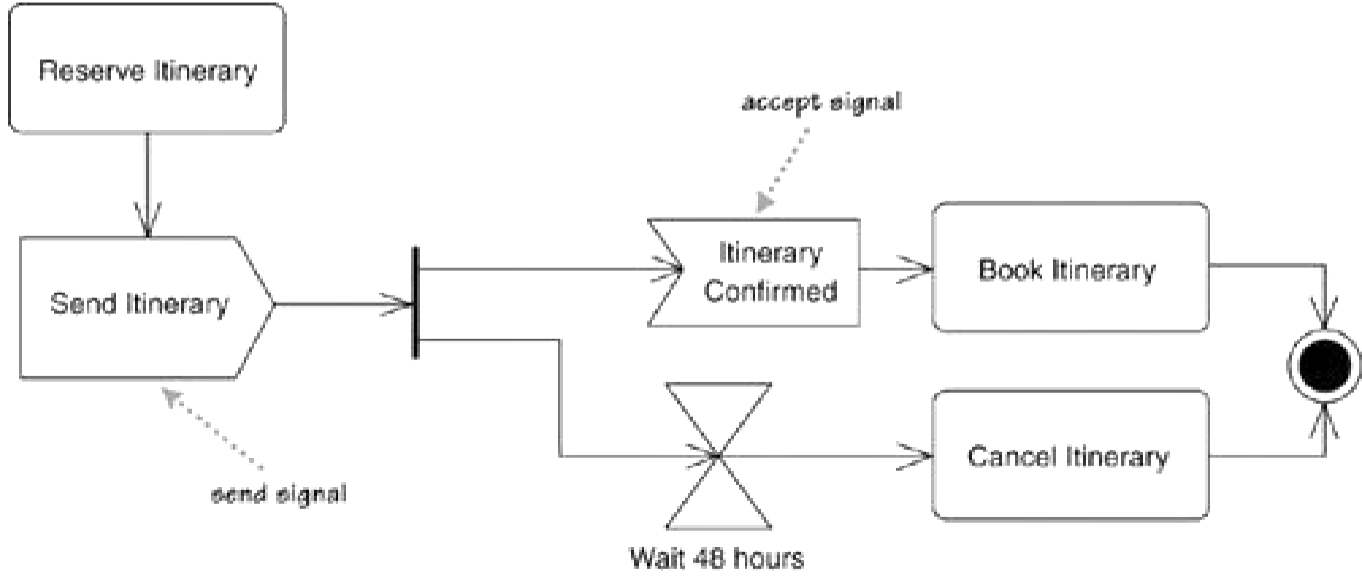
\includegraphics[width=0.5\linewidth]{assets/UML/activity/activity-5.png}}
    \caption{Esempi di utilizzo di \textbf{segnali}}
\end{figure}

\begin{figure}[H]
    \centering
    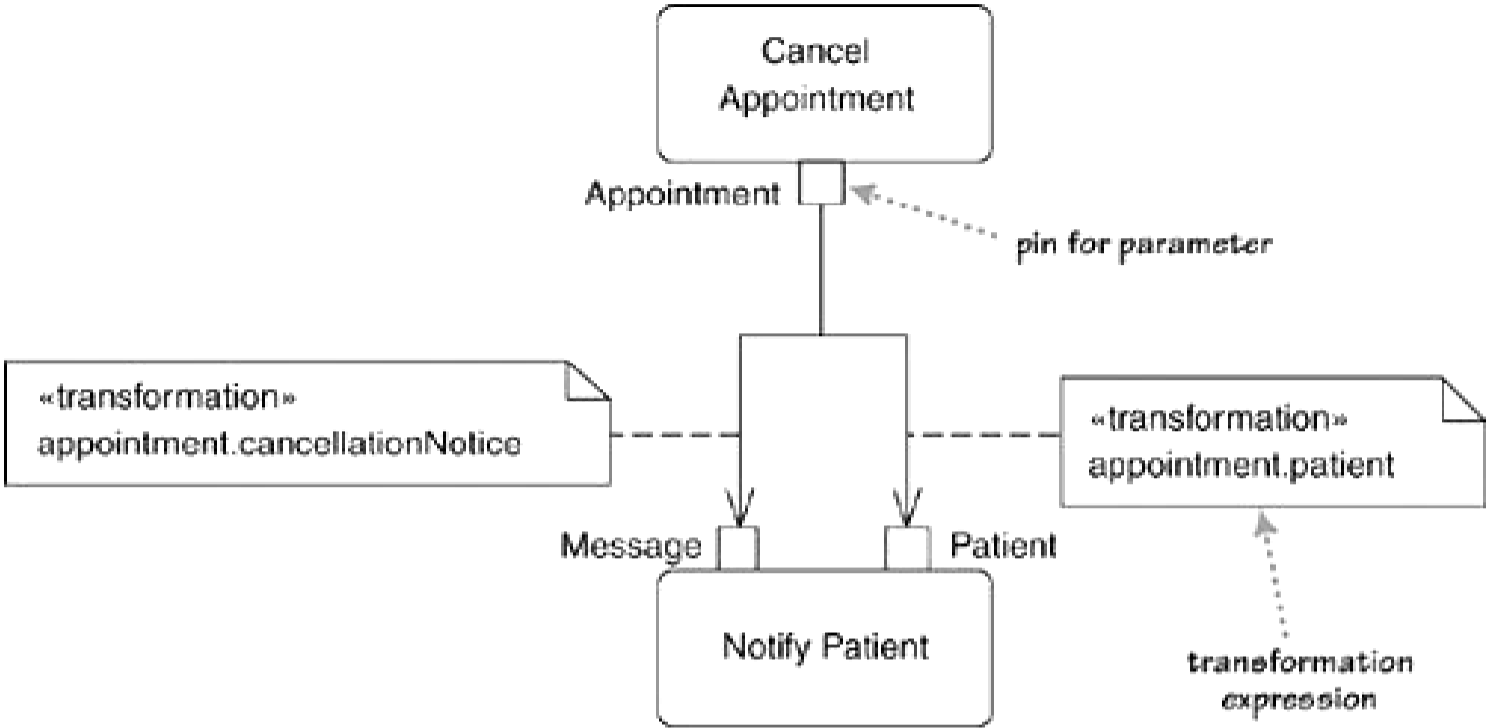
\includegraphics[width=0.75\linewidth]{assets/UML/activity/activity-7.png}
    \caption{I \textbf{pin} consentono di identificare oggetti in input/output per le attività. Le \textbf{trasformazioni} mostrano le modifiche subite dagli oggetti nelle attività.}
\end{figure}

\paragraph{Regione di espansione} Insieme di attività che devono essere eseguite per ogni elemento di una lista di oggetti in ingresso. Restituiscono in output un'altra lista di oggetti.

\begin{figure}[H]
    \centering
    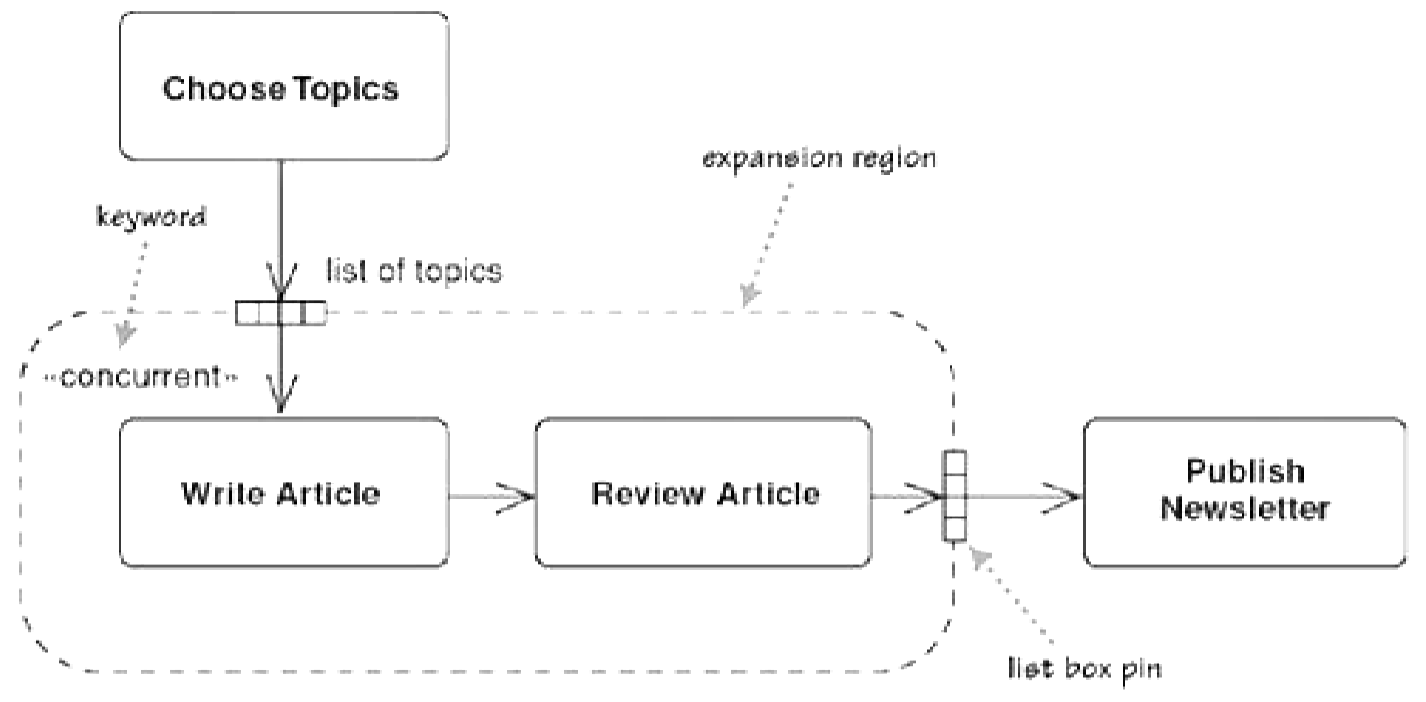
\includegraphics[width=0.8\linewidth]{assets/UML/activity/activity-8.png}
    \caption{Esempio di utilizzo di \textbf{regioni di espansione}}
\end{figure}

\begin{figure}[H]
    \centering
    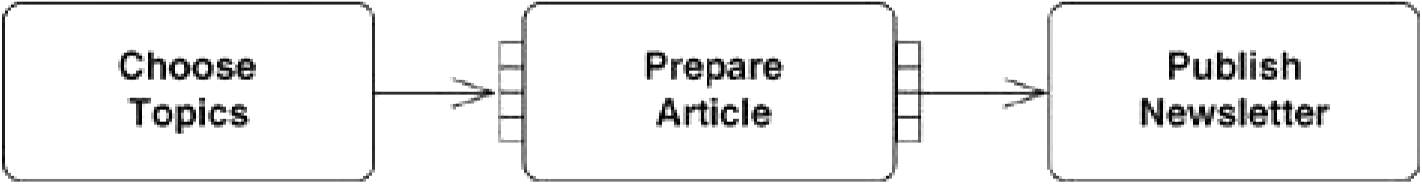
\includegraphics[width=0.8\linewidth]{assets/UML/activity/activity-9.png}
    \caption{Diagramma semplificato risultante a seguito della specifica della regione di espansione}
\end{figure}

\newpage
\subsection{Class}

I \textbf{class diagram} sono i diagrammi UML più utilizzati. Descrivono le \textit{tipologie di oggetti} (classi) che fanno parte del sistema, e le loro relazioni statiche. Nella \textit{prospettiva concettuale} definiscono un vocabolario del dominio applicativo.

\begin{figure}[H]
    \centering
    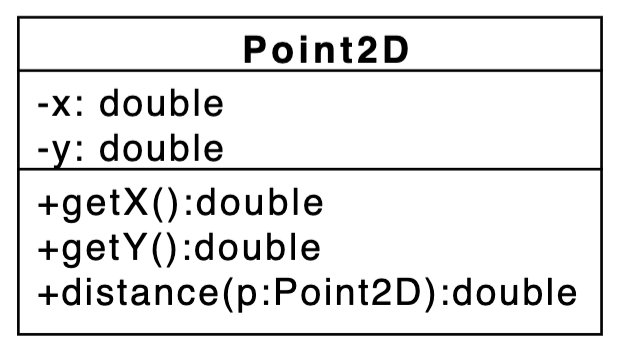
\includegraphics[width=0.5\linewidth]{assets/UML/class/class-1.png}
    \caption{Esempio di definizione di classe}
\end{figure}

\paragraph{Classe} Rappresentata graficamente da rettangoli contenenti almeno il nome della classe e al più le sue caratteristiche. Le caratteristiche (o \textit{feature}) sono divise in \textit{proprietà} e \textit{operazioni}, queste possono avere diversi livelli di visibilità: \textit{public} (+), \textit{private} (-), \textit{protected} (\#) o \textit{package} ($\sim$).

\newpage
\paragraph{Proprietà} Rappresentano le caratteristiche strutturali di una classe (non temporanee, es. parametri in input di un metodo). Si possono esprimere sotto forma di \textit{attributo}:
\begin{center}
    $\langle$visibilità$\rangle$ $\langle$nome$\rangle$ : $\langle$tipo$\rangle$ $\langle$molteplicità$\rangle$ = $\langle$default$\rangle$ \{$\langle$proprietà$\rangle$\}
\end{center}
Dove:
\begin{itemize}
    \item La \textbf{visibilità} è indicata con un simbolo;
    \item Il \textbf{tipo} indica l'insieme di valori assumibili;
    \item La \textbf{molteplicità} vincola il numero di oggetti che possono costituire l'attributo. Espressa come intervallo $[m, n]$;
    \item Il \textbf{default} è valore predefinito;
    \item La \textit{proprietà} è una stringa che indica vincoli aggiuntivi (es. \textit{read-only} o \textit{frozen}). Per specificare il criterio di l'ordinamento si usano \textit{ordered} o \textit{sorted}
\end{itemize}
Si esprimono \textit{attributi} (il cui tipo è non significativo) e \textit{associazioni} (il cui tipo è significativo, espresso da un'altra classe del sistema).
Non esiste un metodo univoco di traduzione, ma in linguaggi moderni quali Java le proprietà corrispondono ai campi (spesso esposti tramite metodi accessori quali \textit{get} e \textit{set} o \textit{wrapper} per collezioni), mentre le operazioni corrispondono ai metodi.

\subparagraph{Proprietà derivata} È una proprietà per la quale non serve introdurre un campo per memorizzarla e può essere calcolata a partire da altre proprietà, è indicata come attributo accompagnato dal simbolo "$/$" corredato da una nota che esprime come ottenerla. Esprime un vicolo (concetto di \textit{invariante di classe}) per le proprietà coinvolte.

\begin{figure}[H]
    \centering
    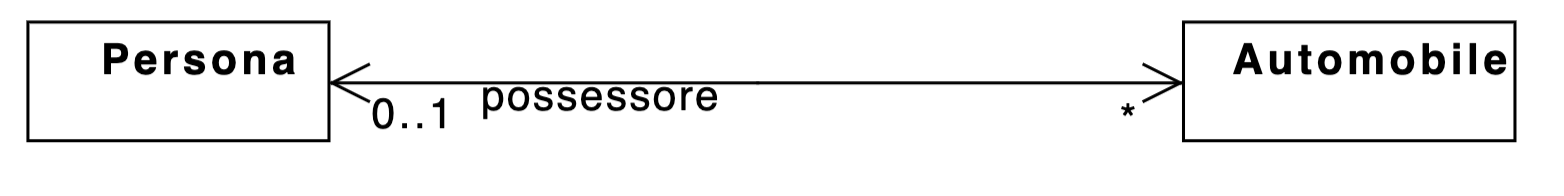
\includegraphics[width=0.75\linewidth]{assets/UML/class/class-3.png}
    \caption{\textbf{Associazione bidirezionale} - ogni oggetto Persona può avere una collezione di oggetti Automobile; ogni oggetto Automobile può avere proprietà opzionale di tipo Persona}
\end{figure}

\newpage
\paragraph{Operazioni} Rappresentano caratteristiche funzionali delle istanze di una classe (azioni invocabili su di esse). Vengono rappresentate tramite stringhe composte come segue:
\begin{center}
        $\langle$visibilità$\rangle$ $\langle$nome$\rangle$(lista\_parametri) : $\langle$tipo\_ritorno$\rangle$ \{$\langle$proprietà$\rangle$\}
\end{center}
La lista dei parametri va specificata. Ogni parametro è separato da virgole ed è espresso come segue:
\begin{center}
        $\langle$direzione$\rangle$ $\langle$nome$\rangle$ : $\langle$tipo$\rangle$ = $\langle$default$\rangle$
\end{center}
Dove:
\begin{itemize}
    \item La \textbf{direzione} indica se il parametro è in input (\textit{in}), in output (\textit{out}) o entrambi (\textit{inout});
    \item La \textbf{proprietà} indica se l'operazione cambia o meno lo stato del sistema. Se non lo cambia si aggiunge la stringa \textit{query}.
\end{itemize}
Nota: Java non permette di specificare la direzione o valore default dei parametri.
UML distingue operazioni (dichiarazione di una procedura) e metodi (corpo dell'operazione).

\subparagraph{Static} Vengono definiti \textit{static} quegli attributi o quelle operazioni che si riferiscono alla classe e non alle sue istanze. Nel diagramma le caratteristiche \textit{static} vengono sottolineate.

\paragraph{Generalizzazione} Anche i class diagram ammettono relazioni di generalizzazione che partono da classi \textit{specializzate} e puntano ad una classe \textit{generale}. In Java viene espressa con il concetto di \textit{ereditarietà} (classe specializzata sottoclasse di classe generica o superclasse - \textbf{Principio di sostituibilità di Liskov}, vedi \ref{liskov}).

\begin{figure}[H]
    \centering
    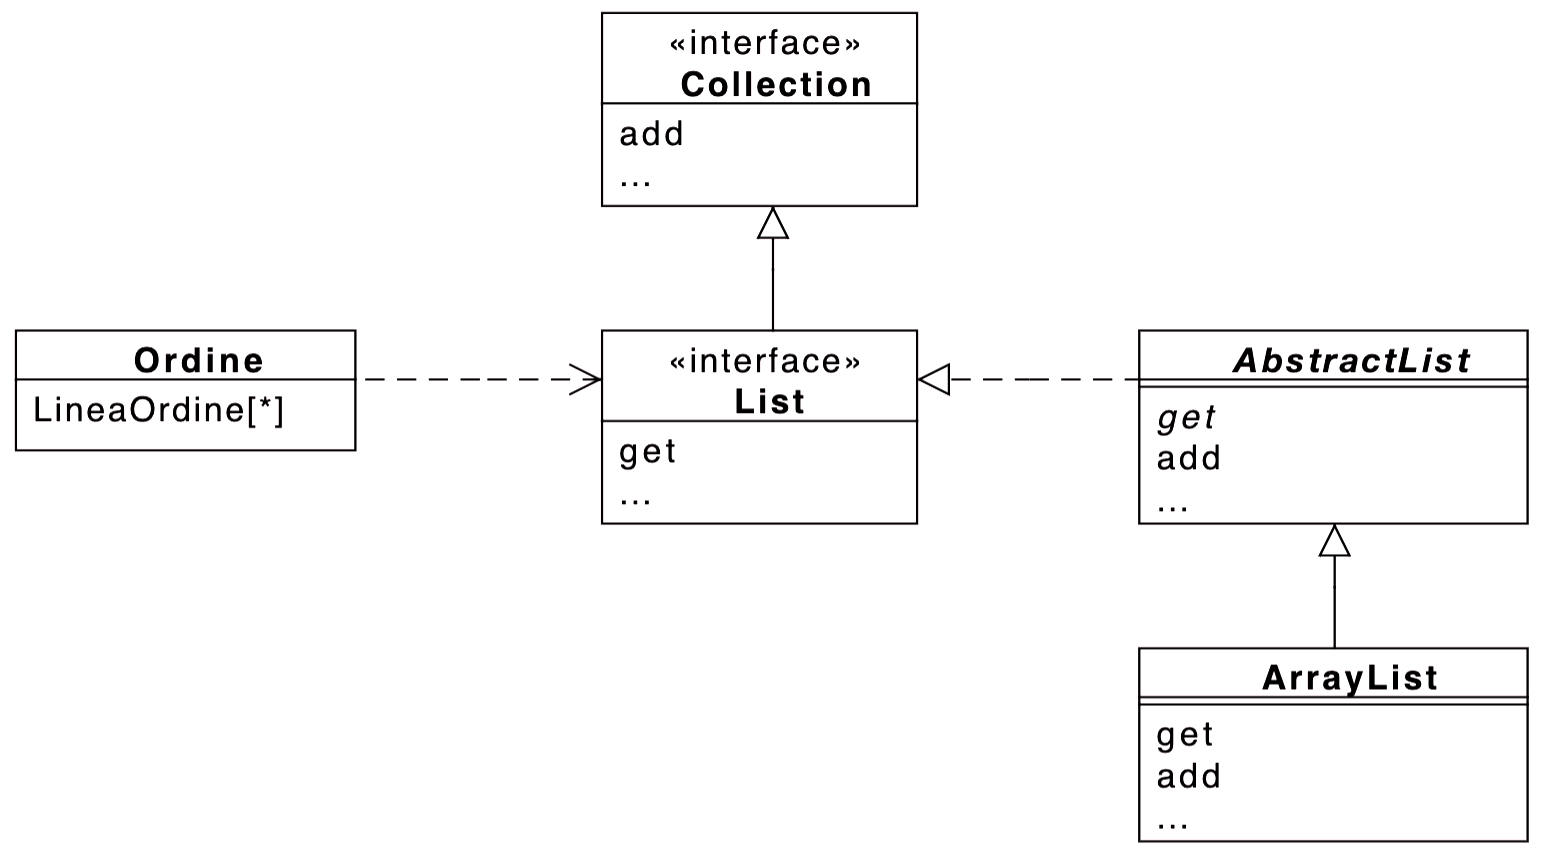
\includegraphics[width=0.75\linewidth]{assets/UML/class/class-8.png}
    \caption{Esempio di generalizzazione}
\end{figure}

\newpage
Di seguito un esempio in Java che non rispetta il principio di Liskov:
\begin{verbatim}
public class Rettangolo {
    private double base;
    private double altezza;

    public void setBase(double b){ base = b;}
    ...
    public double getBase(){return base;}
    ...
    public double getArea(){return base * altezza;}
}

public class Quadrato extends Rettangolo {
    public Quadrato(double l) {
        super(l, l);
    }
    ...
}
\end{verbatim}
Sebbene \textit{geometricamente} un quadrato è un rettangolo, l'implementazione è \textbf{sbagliata} in quanto non deve essere possibile sostituire un Quadrato ad un Rettangolo laddove ci si aspetta il secondo. Si hanno quindi due alternative: rendere le classi \textbf{immutabili} o \textbf{separarle}.

I class diagram ammettono il concetto di \textit{classe astratta} (non istanziabile) e \textit{operazione astratta} (solo dichiarata, priva di corpo), convenzionalmente indicate dal nome scritto in corsivo.

È anche possibile definire delle \textit{interfacce} (insieme di operazioni) indicate dalla parola chiave $\langle\langle$interface$\rangle\rangle$.

La relazione che lega interfaccia e classe (astratta o concreta) si dice \textit{realizzazione} e viene rappresentata da una linea tratteggiata con la punta chiusa e vuota che parte dalla classe e punta all'interfaccia.

\begin{figure}[H]
    \centering
    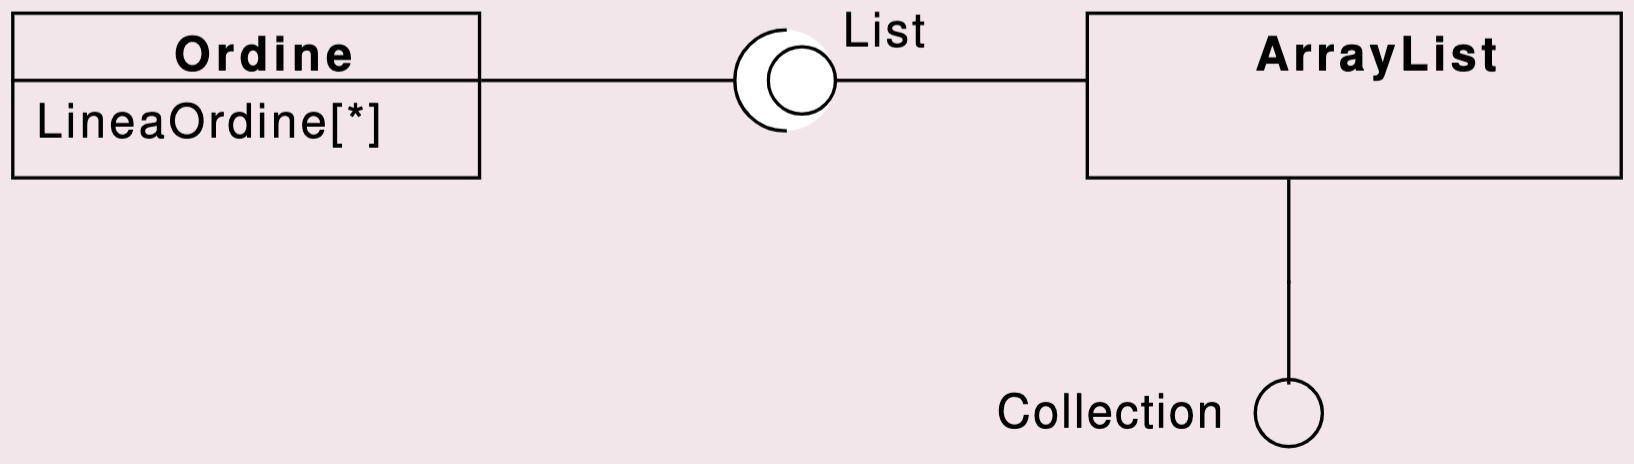
\includegraphics[width=0.75\linewidth]{assets/UML/class/class-9.png}
    \caption{Esempio di utilizzo della notazione \textit{lollipop} (classe fornisce interfaccia) e notazione \textit{socket} (classe richiede interfaccia)}
\end{figure}

\begin{figure}[H]
    \centering
    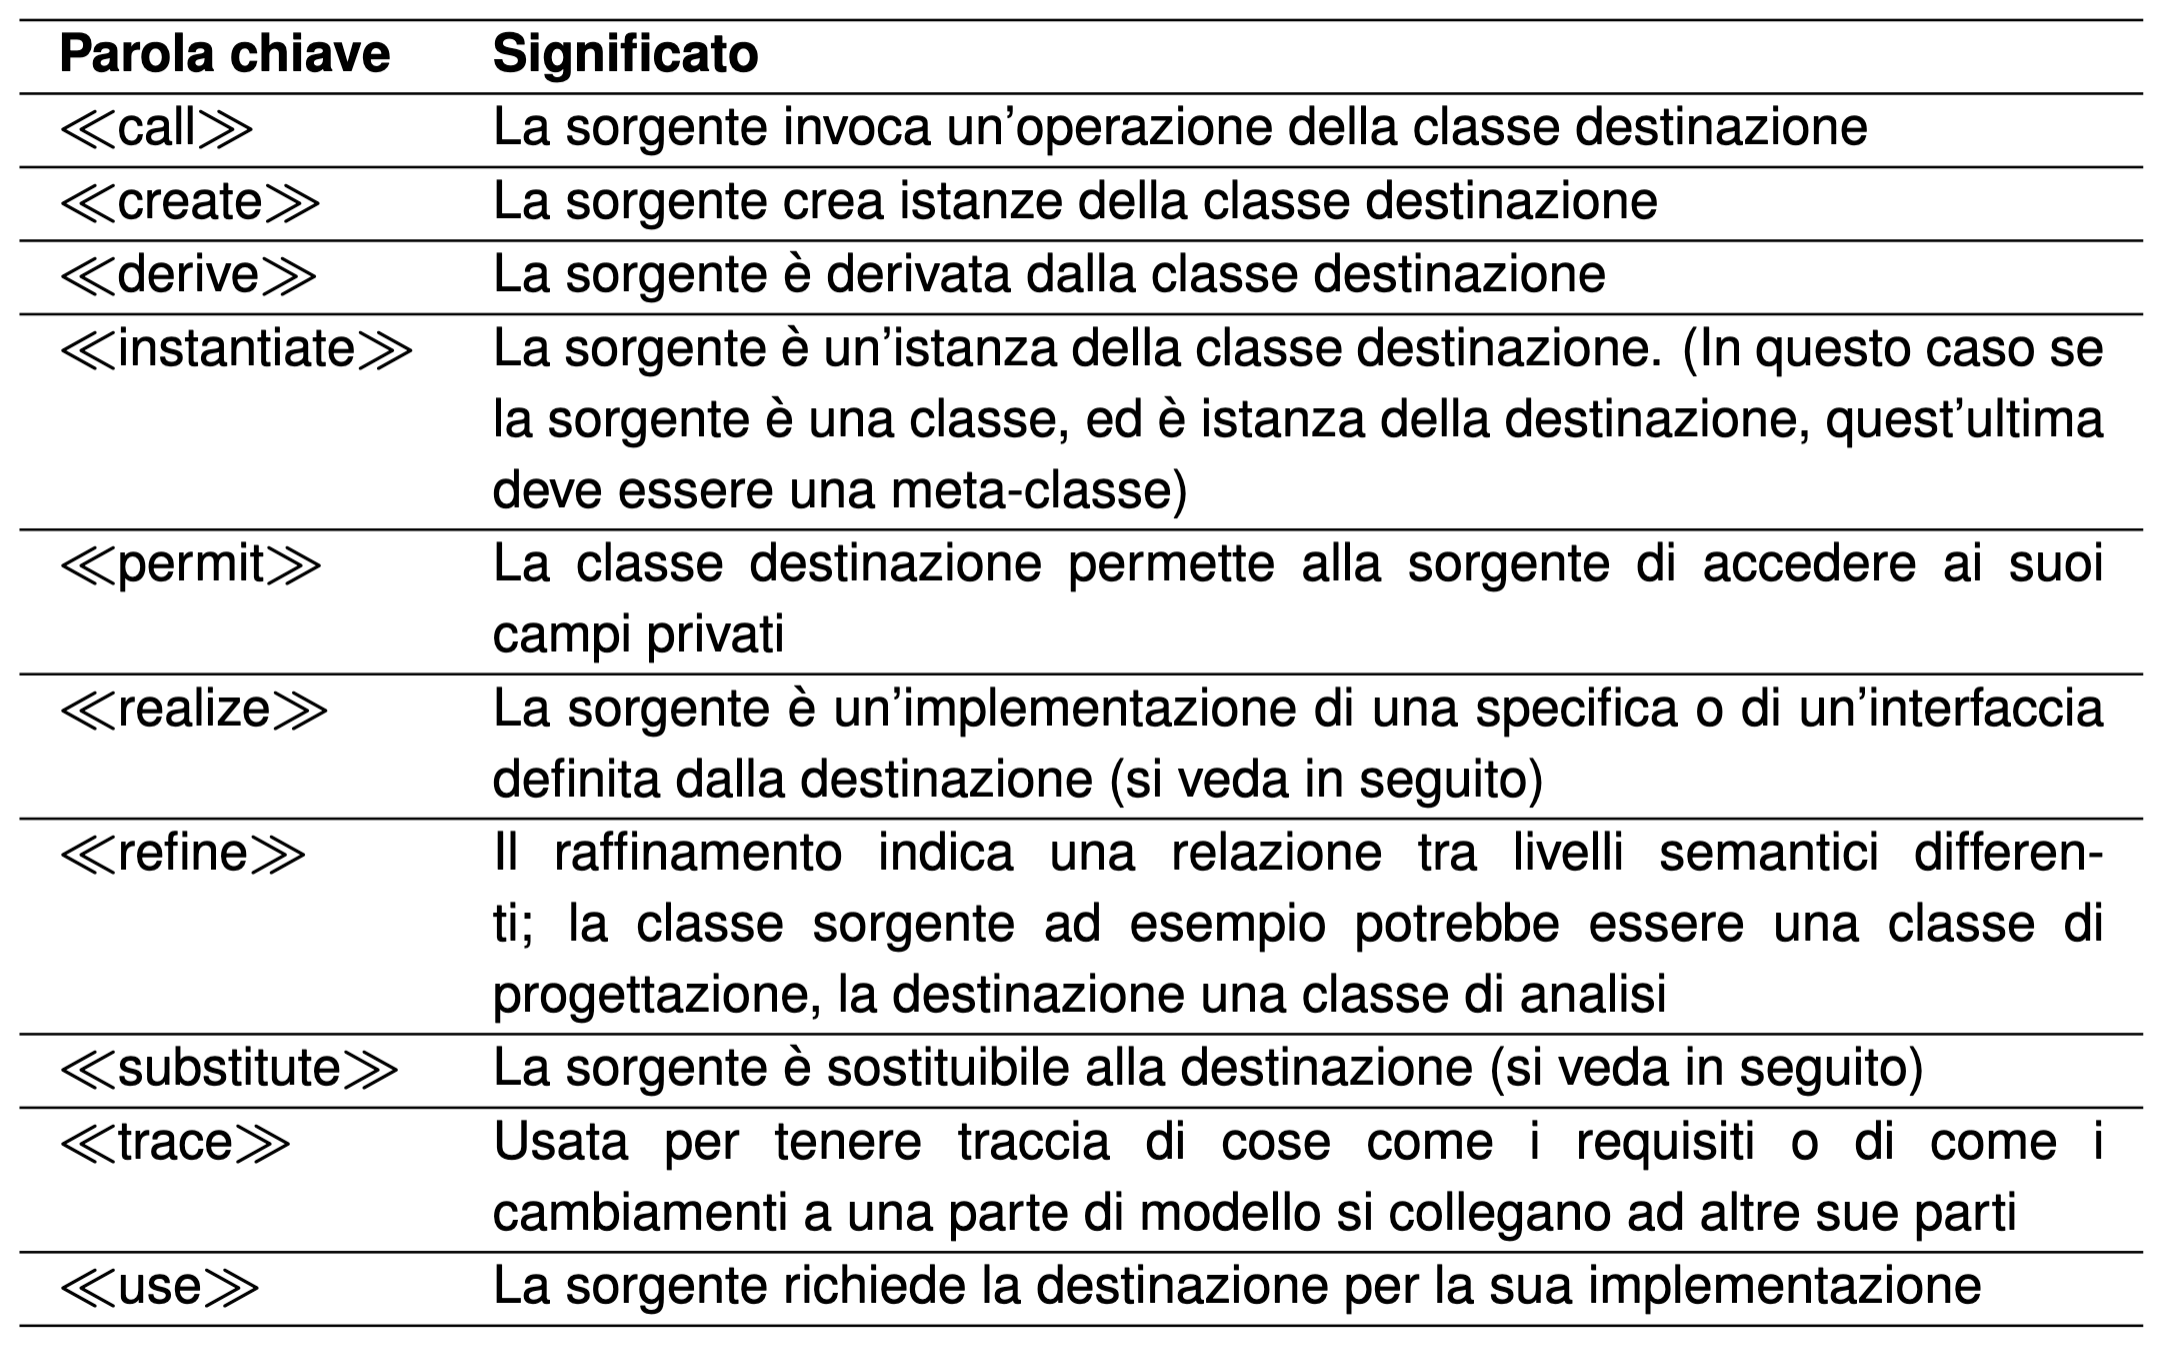
\includegraphics[width=1\linewidth]{assets/UML/class/class-10.png}
    \caption{I class diagram prevedono \textbf{dipendenze}, relazioni unidirezionali tra una classe \textit{client} (da cui parte la freccia) ad una classe \textit{supplier} (in cui punta la freccia). Una qualsiasi modifica alla classe supplier ha effetto sulla classe client (non viceversa), in più NON gode di proprietà transitiva. È inoltre possibile definire dipendenze \textit{custom} (personalizzate)}.
\end{figure}

\begin{figure}[H]
    \centering
    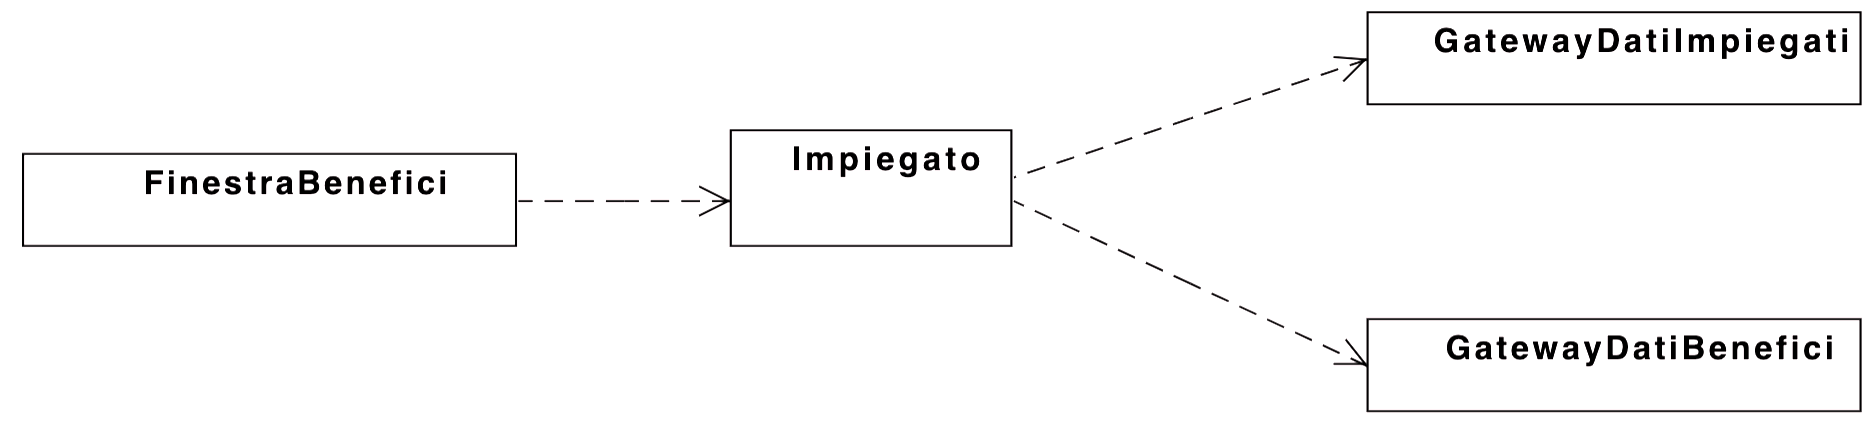
\includegraphics[width=1\linewidth]{assets/UML/class/class-5.png}
    \caption{Esempio di utilizzo del concetto di dipendenza}
\end{figure}

I class diagram consentono l'uso di interfacce e classi \textbf{parametriche}: nel codice, i campi e i parametri/risultati dei metodi sono di tipo generico (sussiste a tempo di compilazione, es. Java) o \textit{template} (sussiste a runtime, es C++).

\begin{figure}[H]
    \centering
    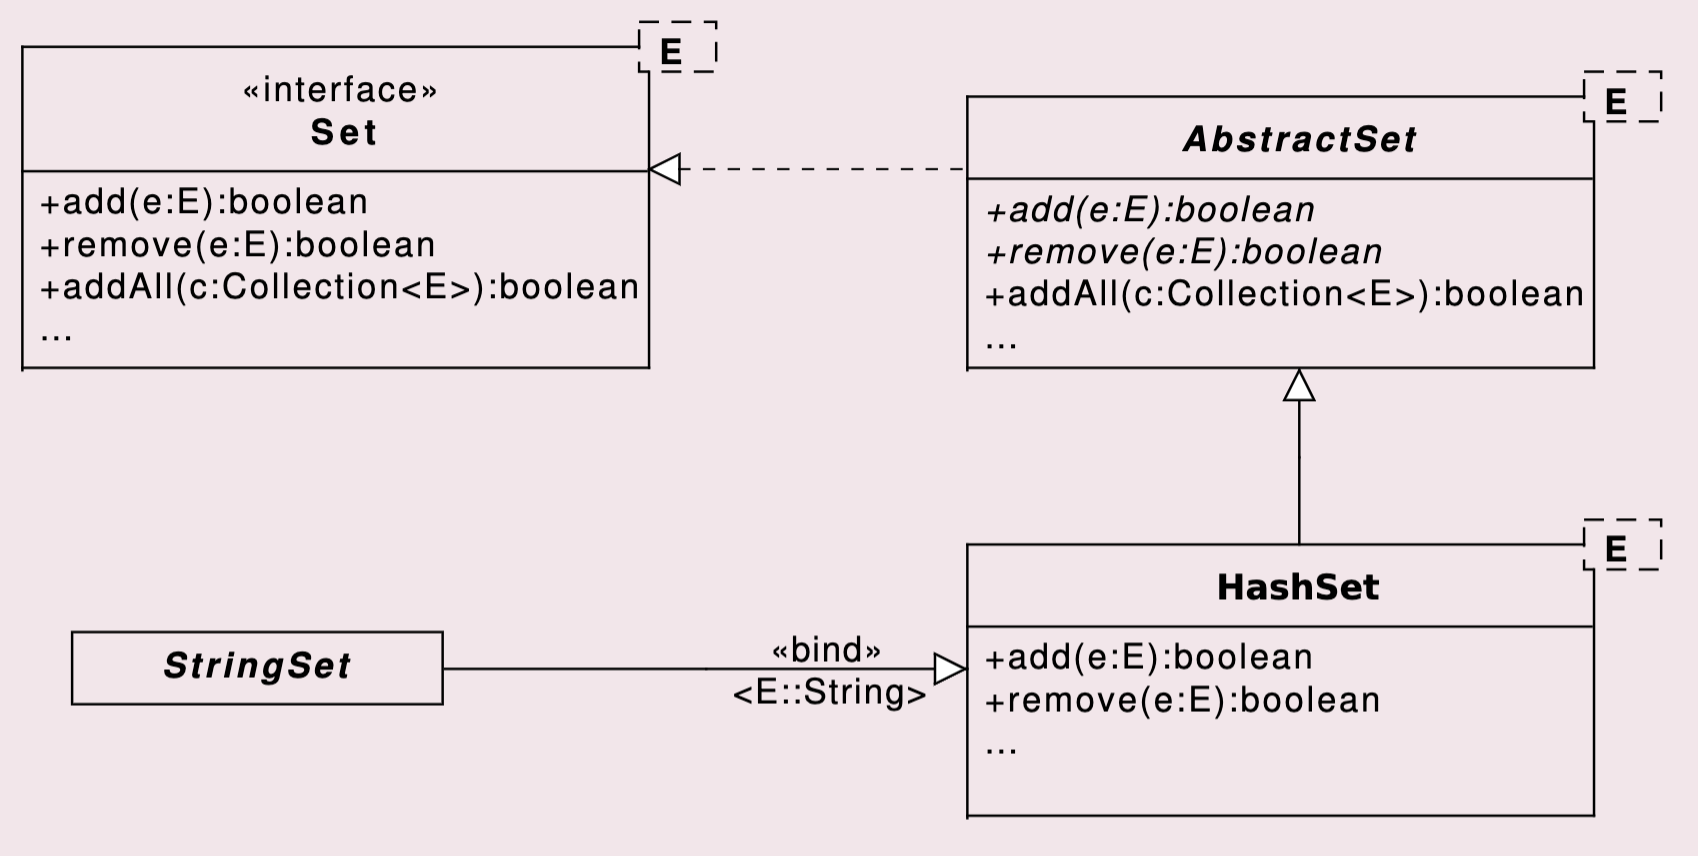
\includegraphics[width=1\linewidth]{assets/UML/class/class-11.png}
    \caption{Esempio di \textbf{derivazione}: classe discendente da una classe parametrica che sostituisce il tipo generico con uno concreto tramite \textit{bind}}
    
\end{figure}
L'introduzione di una classe tramite derivazione fa si che si abbia una relazione di \textit{raffinamento}. 

I tipi che possono assumere solo un set finito di valori prefissati sono modellati tramite \textit{enumerazioni}. 

Una classe \textit{attiva} è una classe che esegue e controlla autonomamente il proprio thread (es. la classe Thread di Java).

\paragraph{Aggregazione} È una forma di associazione in cui l'oggetto destinazione è un \textit{componente} della classe sorgente, il quale viene \textit{aggregato}.

\begin{figure}[H]
    \centering
    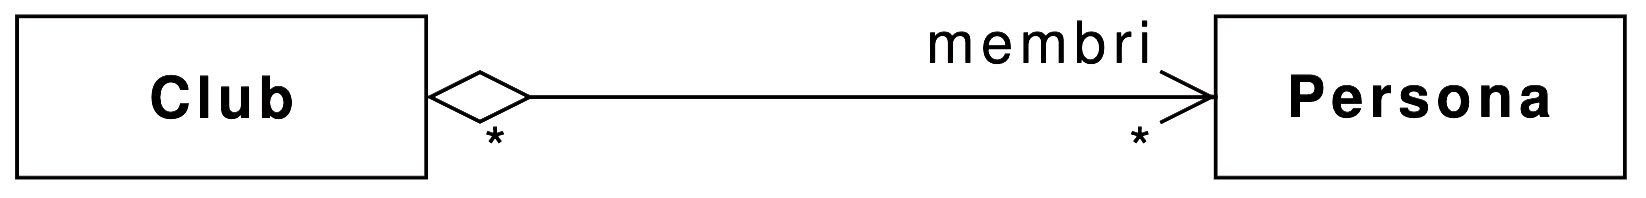
\includegraphics[width=1\linewidth]{assets/UML/class/class-6.png}
    \caption{Esempio di aggregazione}
\end{figure}

\paragraph{Composizione} È una forma di aggregazione in cui l'oggetto sorgente è composto da un insieme di oggetti del tipo destinazione.

\begin{figure}[H]
    \centering
    
\includegraphics[width=1\linewidth]{assets/UML/class/class-7.png}
    \caption{Esempio di composizione}
\end{figure}
Le differenze tra composizione e aggregazione sono le seguenti:
\begin{itemize}
    \item La \textit{composizione} è una relazione esclusiva: l'oggetto componente può far parte di un solo oggetto composto (uno ad uno); nell'\textit{aggregazione} può esistere una relazione uno a molti.
    \item Nella \textit{composizione}, l'istanza composta è responsabile dell'esistenza (creazione, modifica e cancellazione) delle istanze componenti, se viene distrutta anche i suoi componenti vengono distrutti; nell'\textit{aggregazione} l'oggetto componente esiste in maniera indipendente dall'aggregato.
\end{itemize}

\begin{figure}[H]
    \centering
    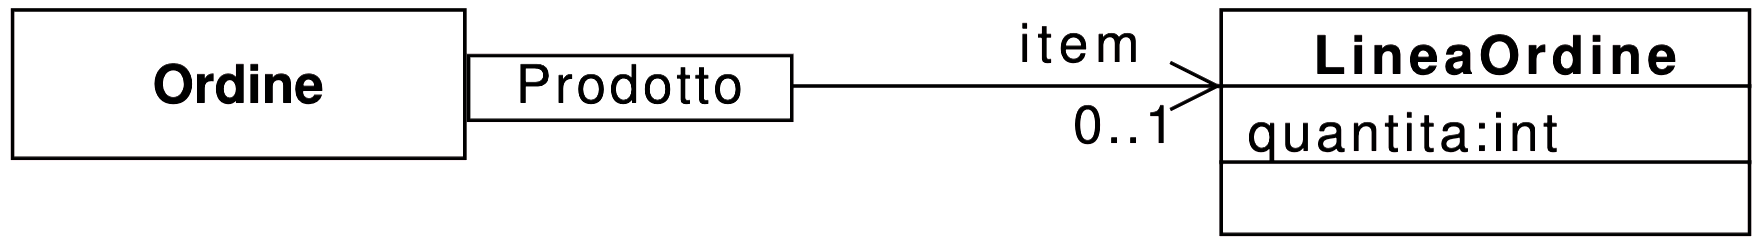
\includegraphics[width=1\linewidth]{assets/UML/class/class-12.png}
    \caption{Esempio di \textbf{associazione qualificata} in cui l'oggetto Ordine possiede più oggetti di tipo LineaOrdine, ma al più uno per ogni oggetto Prodotto (detto \textit{qualificatore}, una sorta di chiave). Implementata tramite array associativi quali mappe, tabelle hash, dizionari, ecc...}
\end{figure}

\vspace{20pt}

\begin{figure}[H]
    \centering
    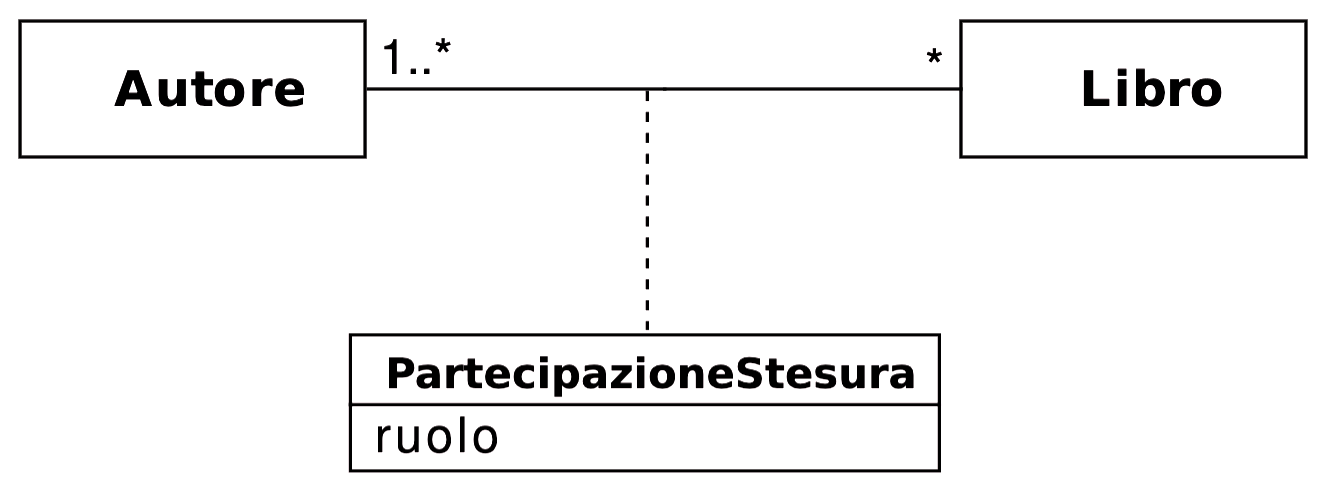
\includegraphics[width=1\linewidth]{assets/UML/class/class-13.png}
    \caption{Esempio di \textbf{classe associativa}: garantisce che per ogni coppia di oggetti associati esista una sola istanza della classe associativa.}
\end{figure}

\vspace{20pt}

\begin{figure}[H]
    \centering
    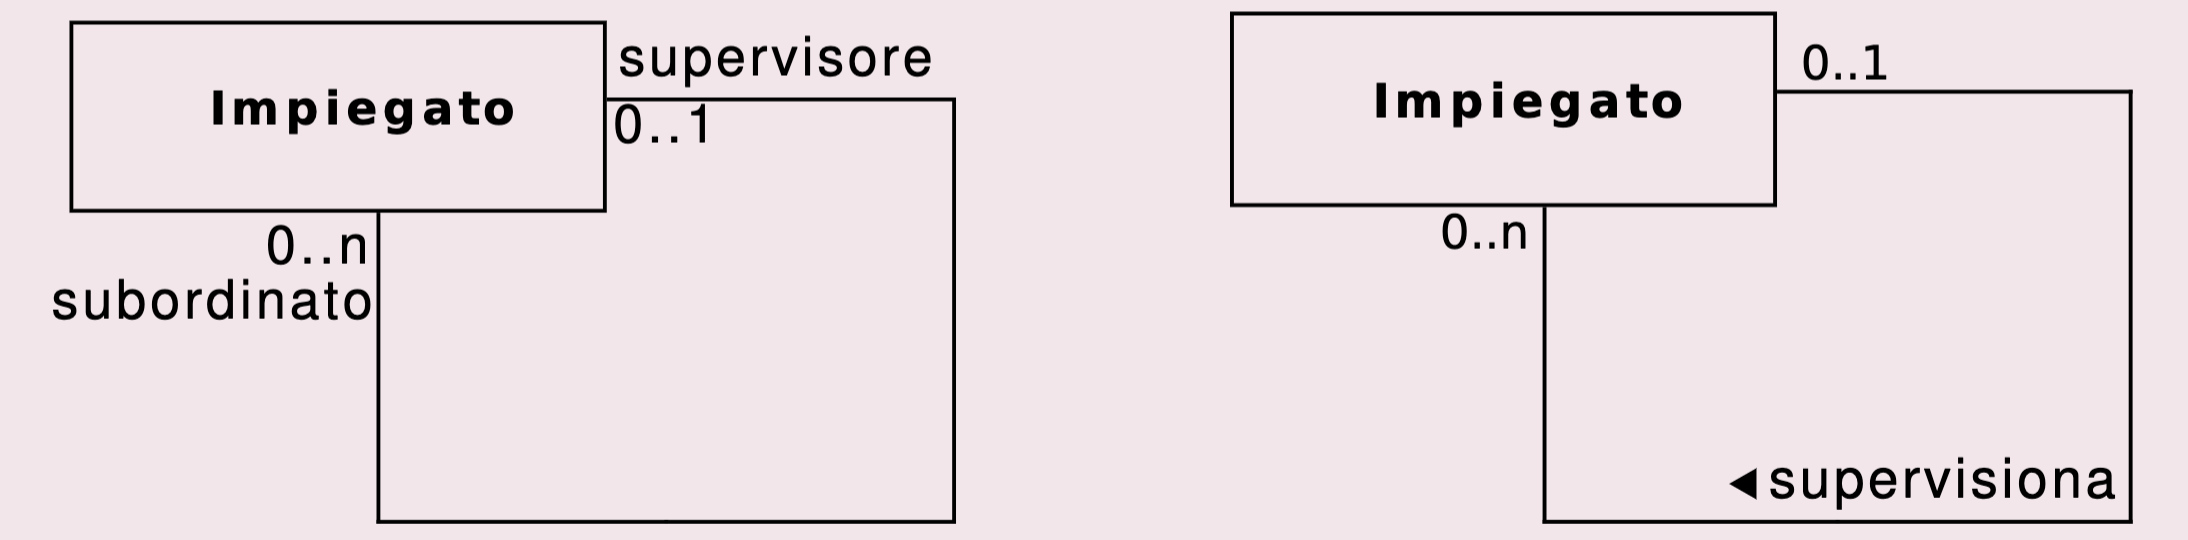
\includegraphics[width=1\linewidth]{assets/UML/class/class-14.png}
    \caption{Esempio di \textbf{associazione riflessiva}: classe sorgente e classe destinazione coincidono, ogni istanza della classe possiede proprietà del suo stesso tipo}
\end{figure}

\vspace{20pt}

\begin{figure}[H]
    \centering
    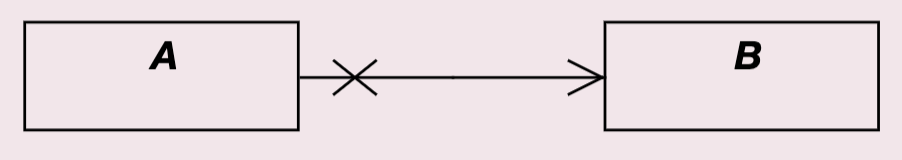
\includegraphics[width=1\linewidth]{assets/UML/class/class-15.png}
    \caption{Concetto di \textbf{non navigabilità}}
\end{figure}

\newpage
\subsection{Communication}

I \textbf{communication diagram}, in maniera simile agli \textit{state diagram}, mostrano il funzionamento collettivo di un gruppo di partecipanti. L'enfasi è posta sui \textbf{messaggi scambiati} (non sul ciclo di vita) e sulle attività svolte da ciascun partecipante.

\paragraph{Partecipante} È un'\textbf{entità del dominio applicativo} nella \textit{prospettiva concettuale}, un \textbf{oggetto} nella \textit{prospettiva software}. Rappresentato da box con angoli smussati. I box sono collegati da linee continue, le quali possono:
\begin{itemize}
    \item tradurre associazioni statiche (tra partecipanti, \textit{compile-time})
    \item introdurre associazioni dinamiche (tra partecipanti, nascono e muoiono a \textit{run-time})
\end{itemize}

\paragraph{Messaggio} Rappresentato da frecce etichettate con l'azione corrispondente e numerato in maniera nidificata. Si usa:
\begin{itemize}
    \item $\langle\langle$create$\rangle\rangle$ per la creazione di partecipanti
    \item $\langle\langle$delete$\rangle\rangle$ per la distruzione di partecipanti
\end{itemize}
Inoltre, è possibile inserire lettere nelle etichette per indicare il thread che esegue l'operazione.

\begin{figure}[H]
    \centering
    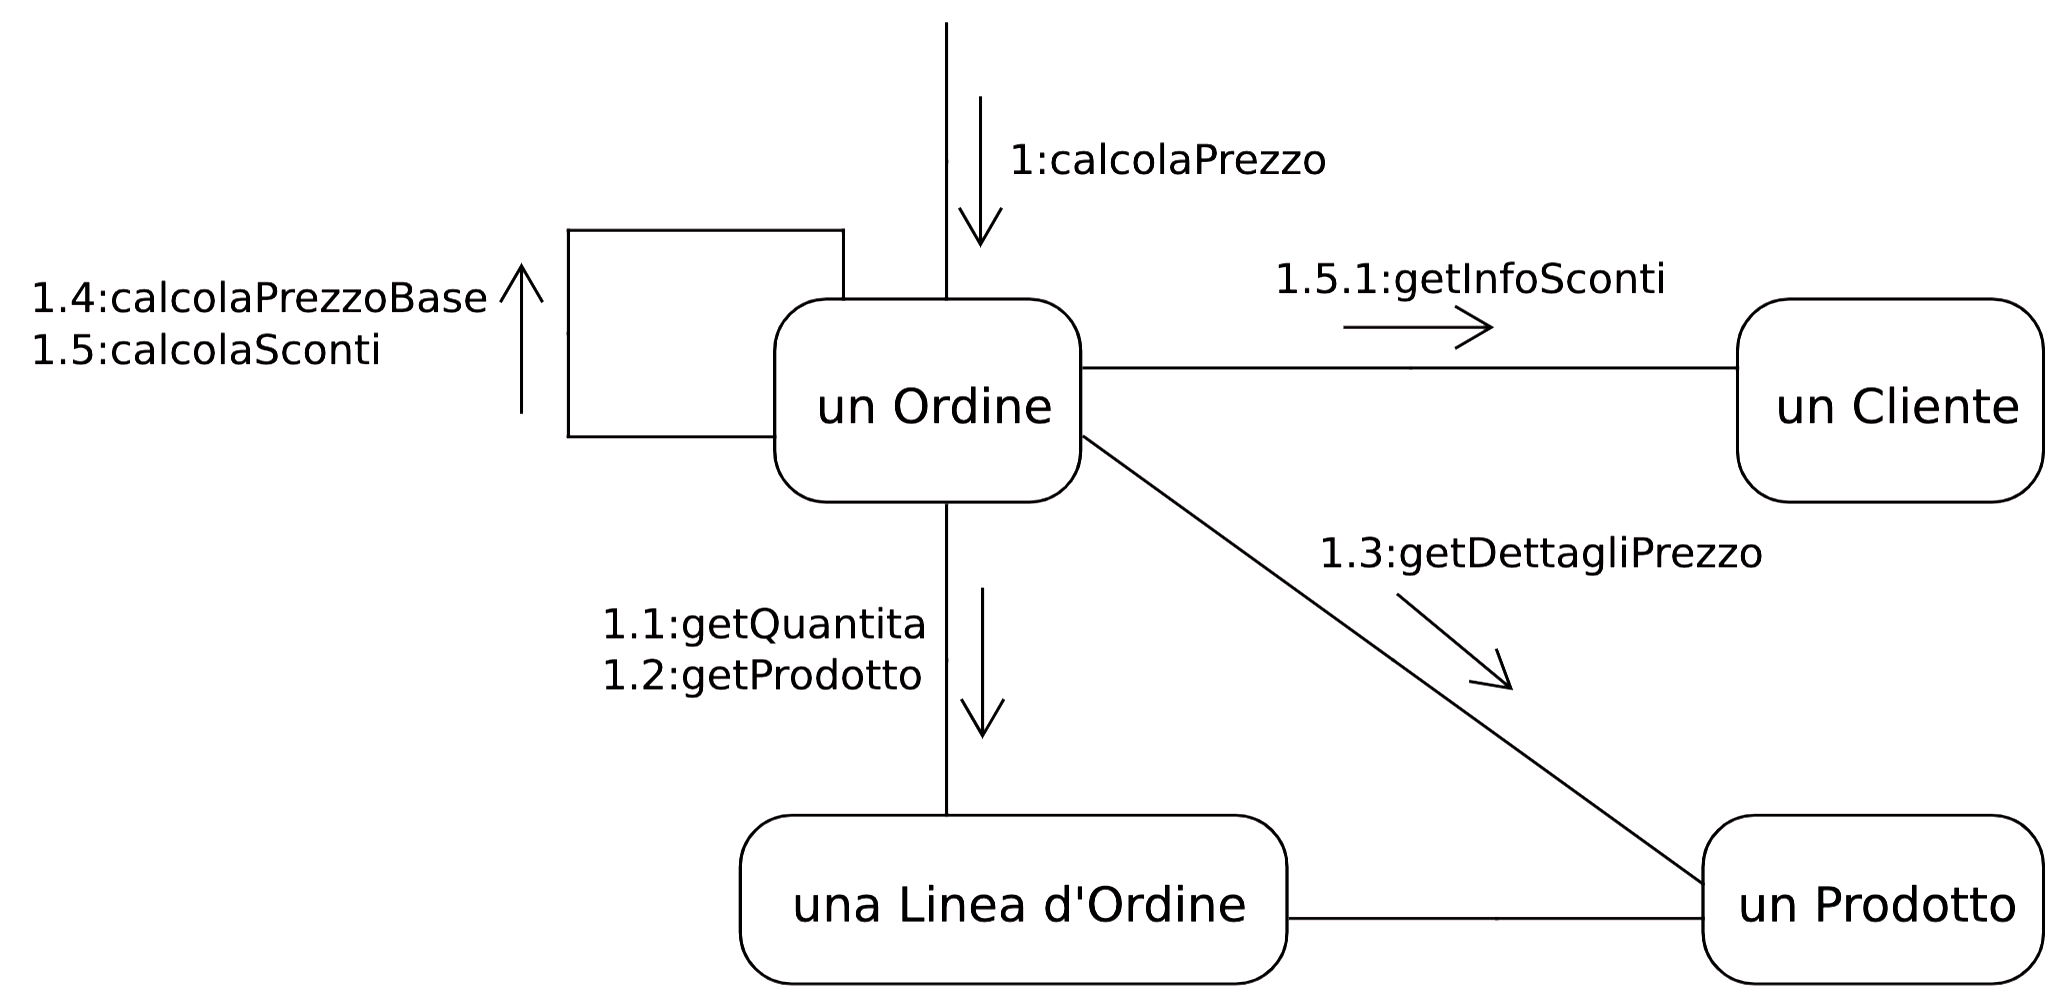
\includegraphics[width=0.75\linewidth]{assets/UML/communication/communication-1.png}
    \caption{Esempio di communication diagram a \textit{controllo centralizzato}.}
\end{figure}

\newpage
\subsection{Componenti}

Uno degli argomenti più dibattuti nella POO è la differenza tra i concetti di \textit{classe} e \textit{componente}. Si può dire che un \textit{componente} è un'entità dotata di interfaccia standard, potenzialmente sostituibile da un altro componente dotato di interfaccia simile (che offre le stesse funzionalità). Un componente può coincidere con: una classe, una porzione di essa o un insieme di classi.

\begin{figure}[H]
    \centering
    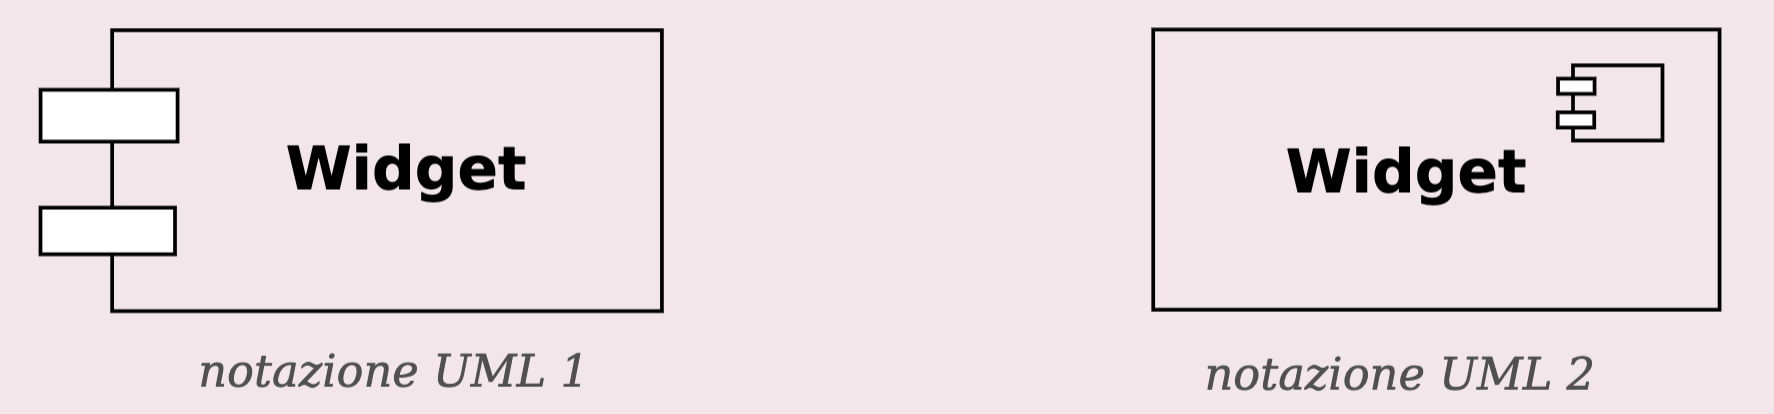
\includegraphics[width=0.75\linewidth]{assets/UML/component/component-1.png}
    \caption{Notazione del componente nelle versioni UML. Un componente complesso può essere rappresentato come struttura composita.}
\end{figure}

\paragraph{Nota} I collegamenti tra componenti sono basati sulle interfacce fornite e richieste.

\begin{figure}[H]
    \centering
    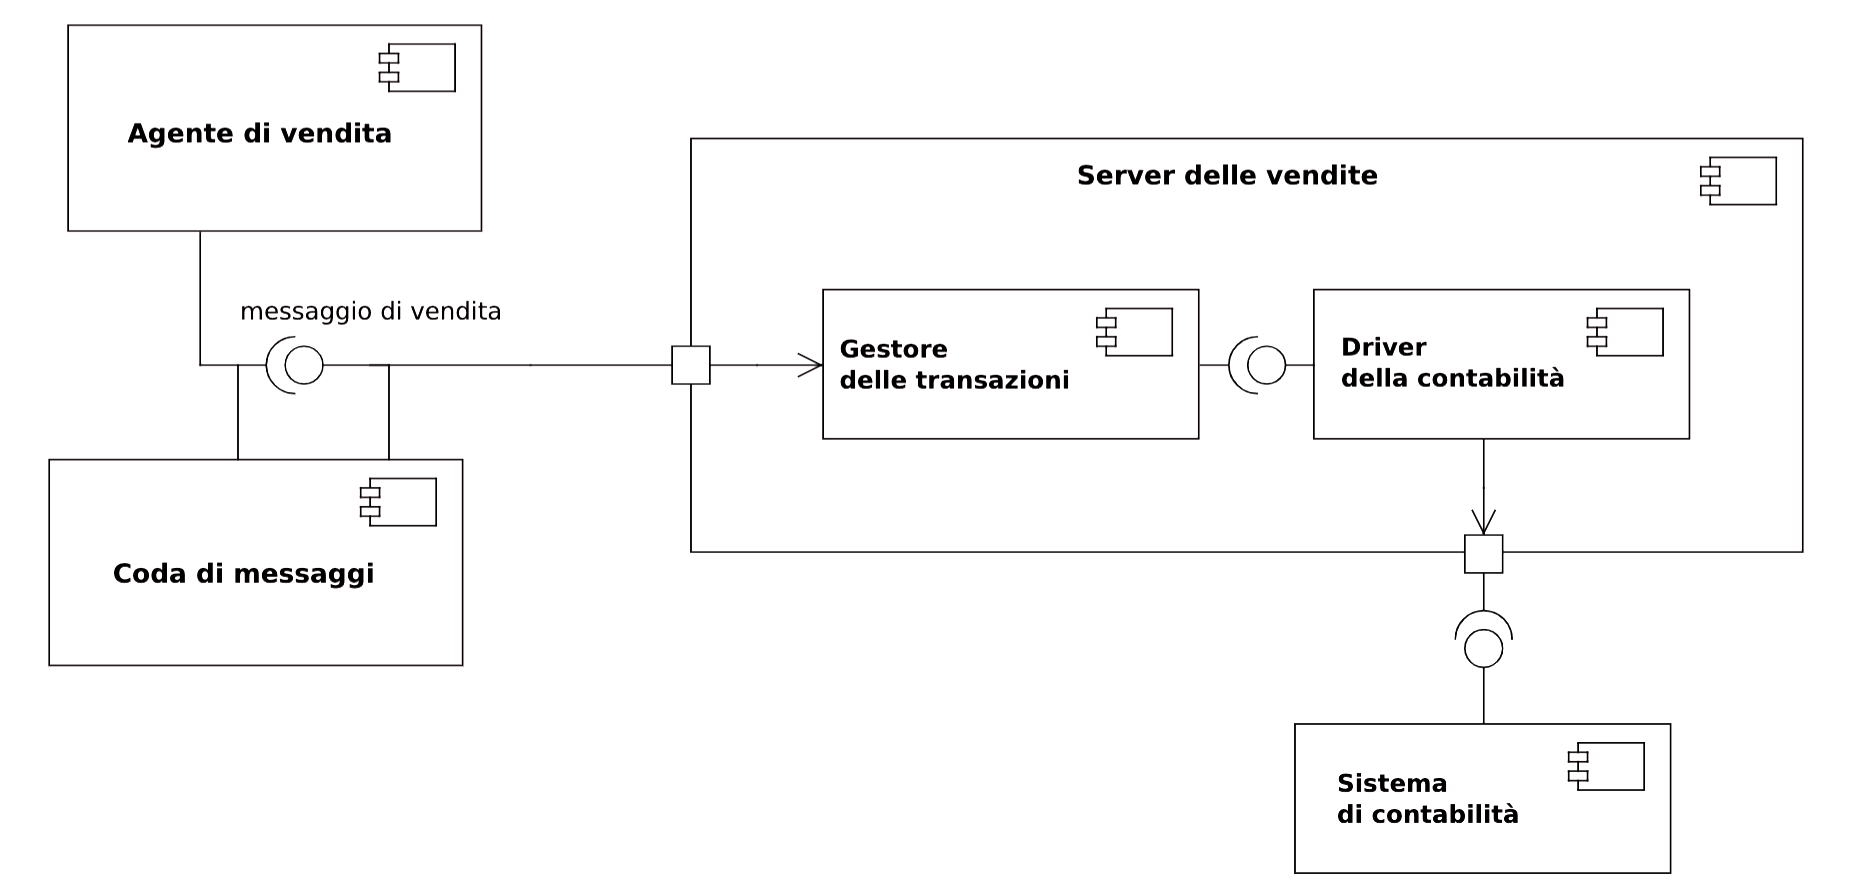
\includegraphics[width=0.75\linewidth]{assets/UML/component/component-2.png}
    \caption{Esempio di component diagram. L'agente di vendita comunica con il server se la rete è disponibile, con la coda altrimenti.}
\end{figure}

\newpage
\subsection{Deployment}

I \textbf{deployment diagram} rappresentano la disposizione fisica dei componenti del sistema software nel contesto applicativo. Il loro modello è rappresentato come un insieme di \textit{nodi}.

\paragraph{Nodo} Contiene uno o più elaborati (\textit{artifact}): manifestazioni fisiche del sistema software (eseguibili, script di configurazione, librerie, jar, file di dati, documenti HTML, ecc...)

I nodi sono collegati da linee continue dette \textit{path} che forniscono informazioni sulla comunicazione tra essi (es. canale usato, protocollo adottato). I valori di etichetta (o \textit{tagged values}) specificano proprietà aggiuntive sui nodi.

\begin{figure}[H]
    \centering
    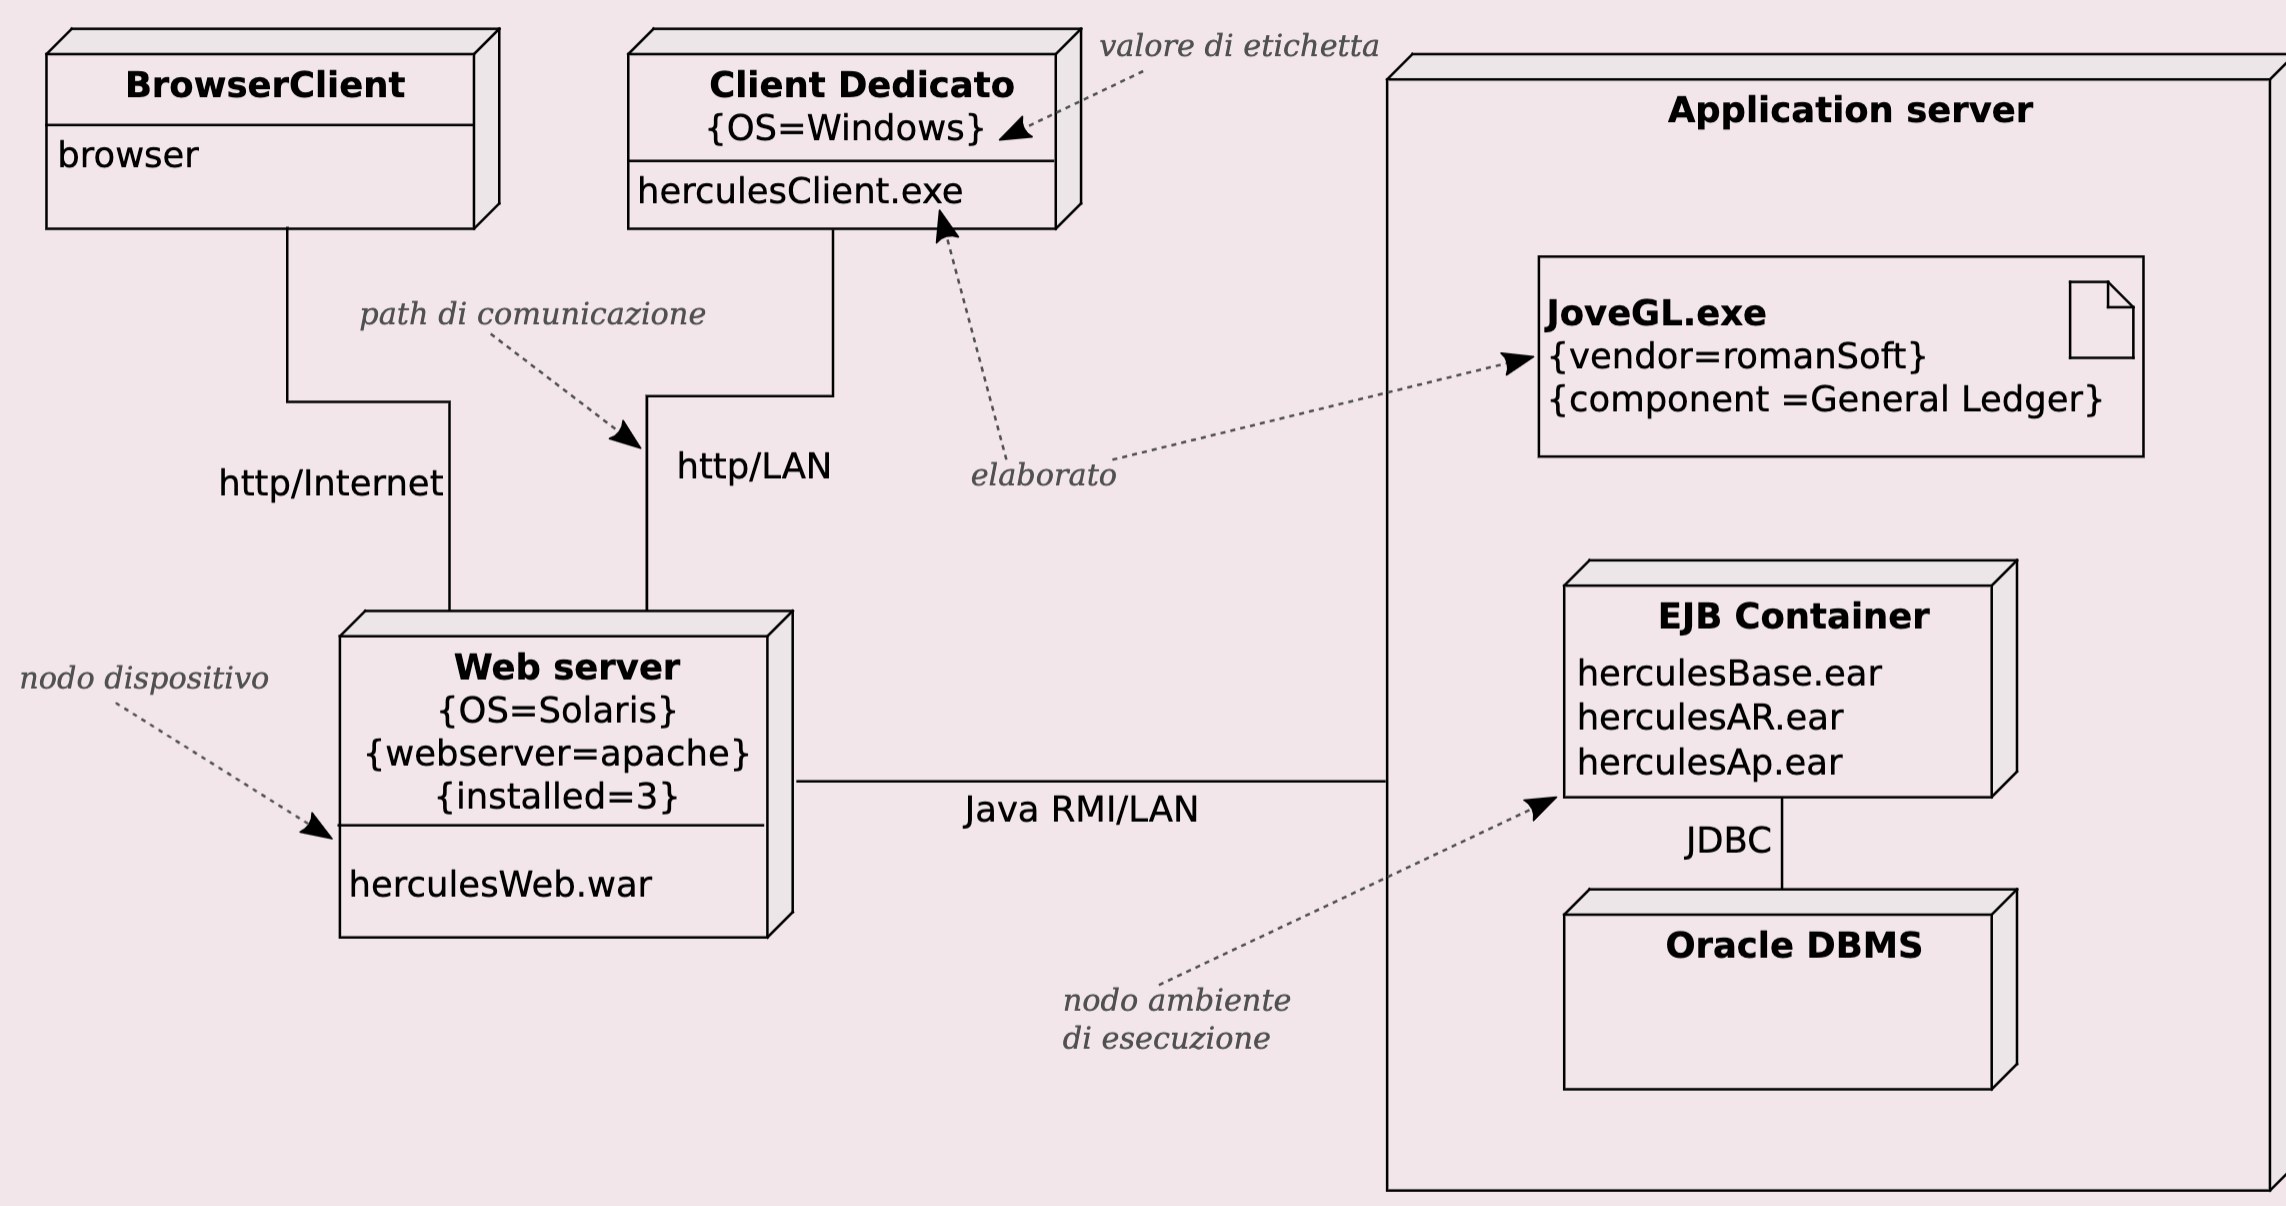
\includegraphics[width=1\linewidth]{assets/UML/deployment/deployment.png}
    \caption{Esempio di deployment diagram}
\end{figure}

\newpage
\newpage
\subsection{Object}

Gli \textbf{object diagram} rappresentano gli oggetti del sistema: specifiche di istanze di classi.

\paragraph{Oggetto} Rappresentato da box con la seguente intestazione:
\begin{center}
    $\langle$nomeOggetto$\rangle$ : $\langle$nomeClasse$\rangle$
\end{center}
Sono collegati tra loro da linee continue dette \textit{link 1-a-1} (istanze di associazioni).

\begin{figure}[H]
    \centering
    \subfloat[Class Diagram]{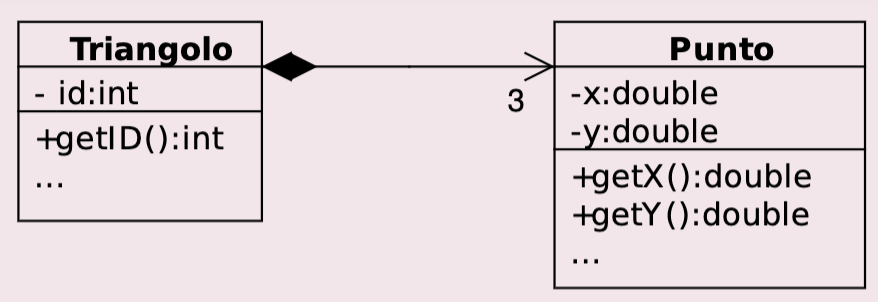
\includegraphics[width=0.6\linewidth]{assets/UML/class/class-2.png}}
    \hfill
    \subfloat[Object Diagram]{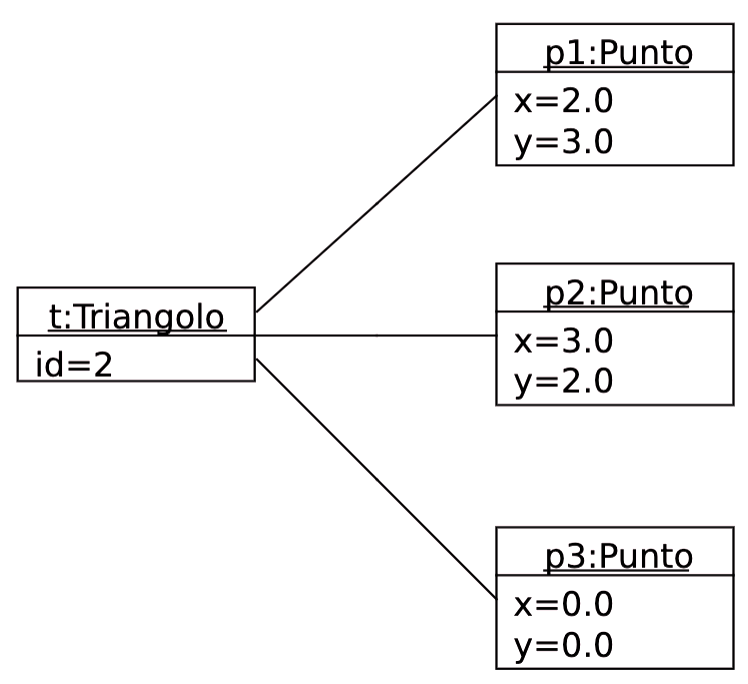
\includegraphics[width=0.3\linewidth]{assets/UML/object/object-1.png}}
    \caption{Differenze tra classi e oggetti in UML}
\end{figure}

\paragraph{Note} È possibile \textit{omettere degli attributi} oppure \textit{mostrare istanze di classi astratte}.

\paragraph{Relazioni} Nonostante il cambio di prospettiva dalle classi agli oggetti, le relazioni illustrate da un object diagram sono sempre di tipo \textit{statico}: il diagramma è una sorta di “fotografia congelata nel tempo”; mostra gli oggetti che costituiscono il sistema in un determinato momento.

\begin{figure}[H]
    \centering
    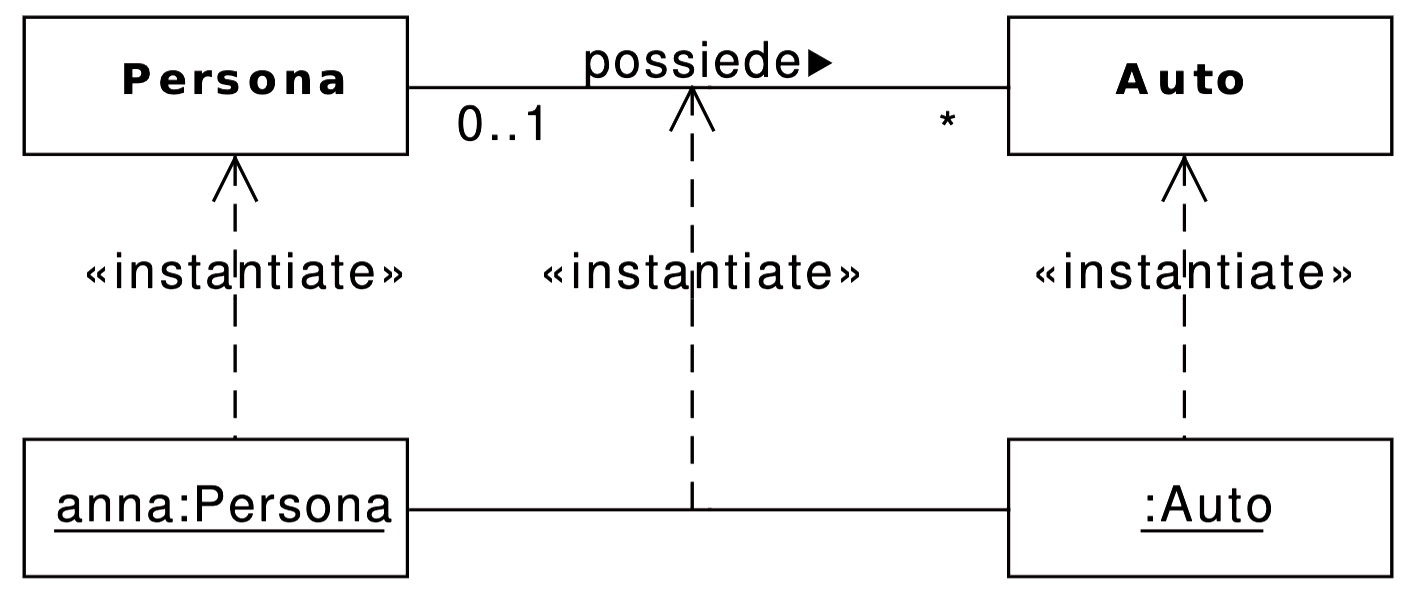
\includegraphics[width=0.75\linewidth]{assets/UML/object/object-2.png}
    \caption{La relazione di dipendenza $\langle$$\langle$instantiate$\rangle$$\rangle$ indica esplicitamente che gli oggetti sono istanze di classi ed il link è un'istanza della relazione \textit{possiede}.}
\end{figure}

\newpage
\subsection{Package}

\newpage
\subsection{Sequence}

\newpage
\subsection{State}

Lo \textbf{state diagram} descrive entità/oggetti il cui comportamento può cambiare dinamicamente nel tempo in relazione a determinati eventi o messaggi ricevuti.

Se la risposta dell'oggetto ad uno stimolo esterno non dipende unicamente dal suo stato corrente (valore dei campi), ma anche dalla sua storia (azioni passate eseguite in risposta a messaggi precedenti), si dice che l'oggetto possiede degli \textbf{stati di controllo}.

\paragraph{Automa a stati finiti} Se il numero di possibili risposte alle sollecitazioni è finito l'oggetto possiede un \textbf{automa a stati finiti} (es. iterator), ovvero un grafo orientato i cui nodi sono stati di controllo e i cui archi rappresentano le \textbf{transizioni di stato}.
Nell'approccio object-oriented un automa a stati finiti è associato a una classe e modella in maniera formale il comportamento delle sue istanze partendo da una specifica informale.

\paragraph{Stato iniziale} Lo stato di controllo in cui l'oggetto viene a trovarsi subito dopo la creazione: viene specificato tramite una \textbf{pseudo-transizione} che emana da un cerchietto nero (\textit{pseudo-stato}).

\paragraph{Stati finali} Nodi dai quali non si hanno transizione. Una transizione di stato è causata da un evento (\textit{trigger}). Si possono specificare delle \textbf{azioni} (operazioni atomiche non interrompibili). A seconda del modo distinguiamo fra:
\begin{itemize}

    \item \textbf{1. Automi di Mealy} in cui le azioni sono associate alle transizioni. Un'azione viene eseguita SEMPRE E SOLO in risposta al trigger della transizione a cui è associata;

    \item  \textbf{2. Automi di Moore} in cui le azioni sono associate agli stati. Un'azione viene eseguita quando l'automa si trova nello stato di controllo a cui è associata, a prescindere dalla transizione che ha portato in quello stato.

\end{itemize}


\begin{figure}[H]
    \centering
    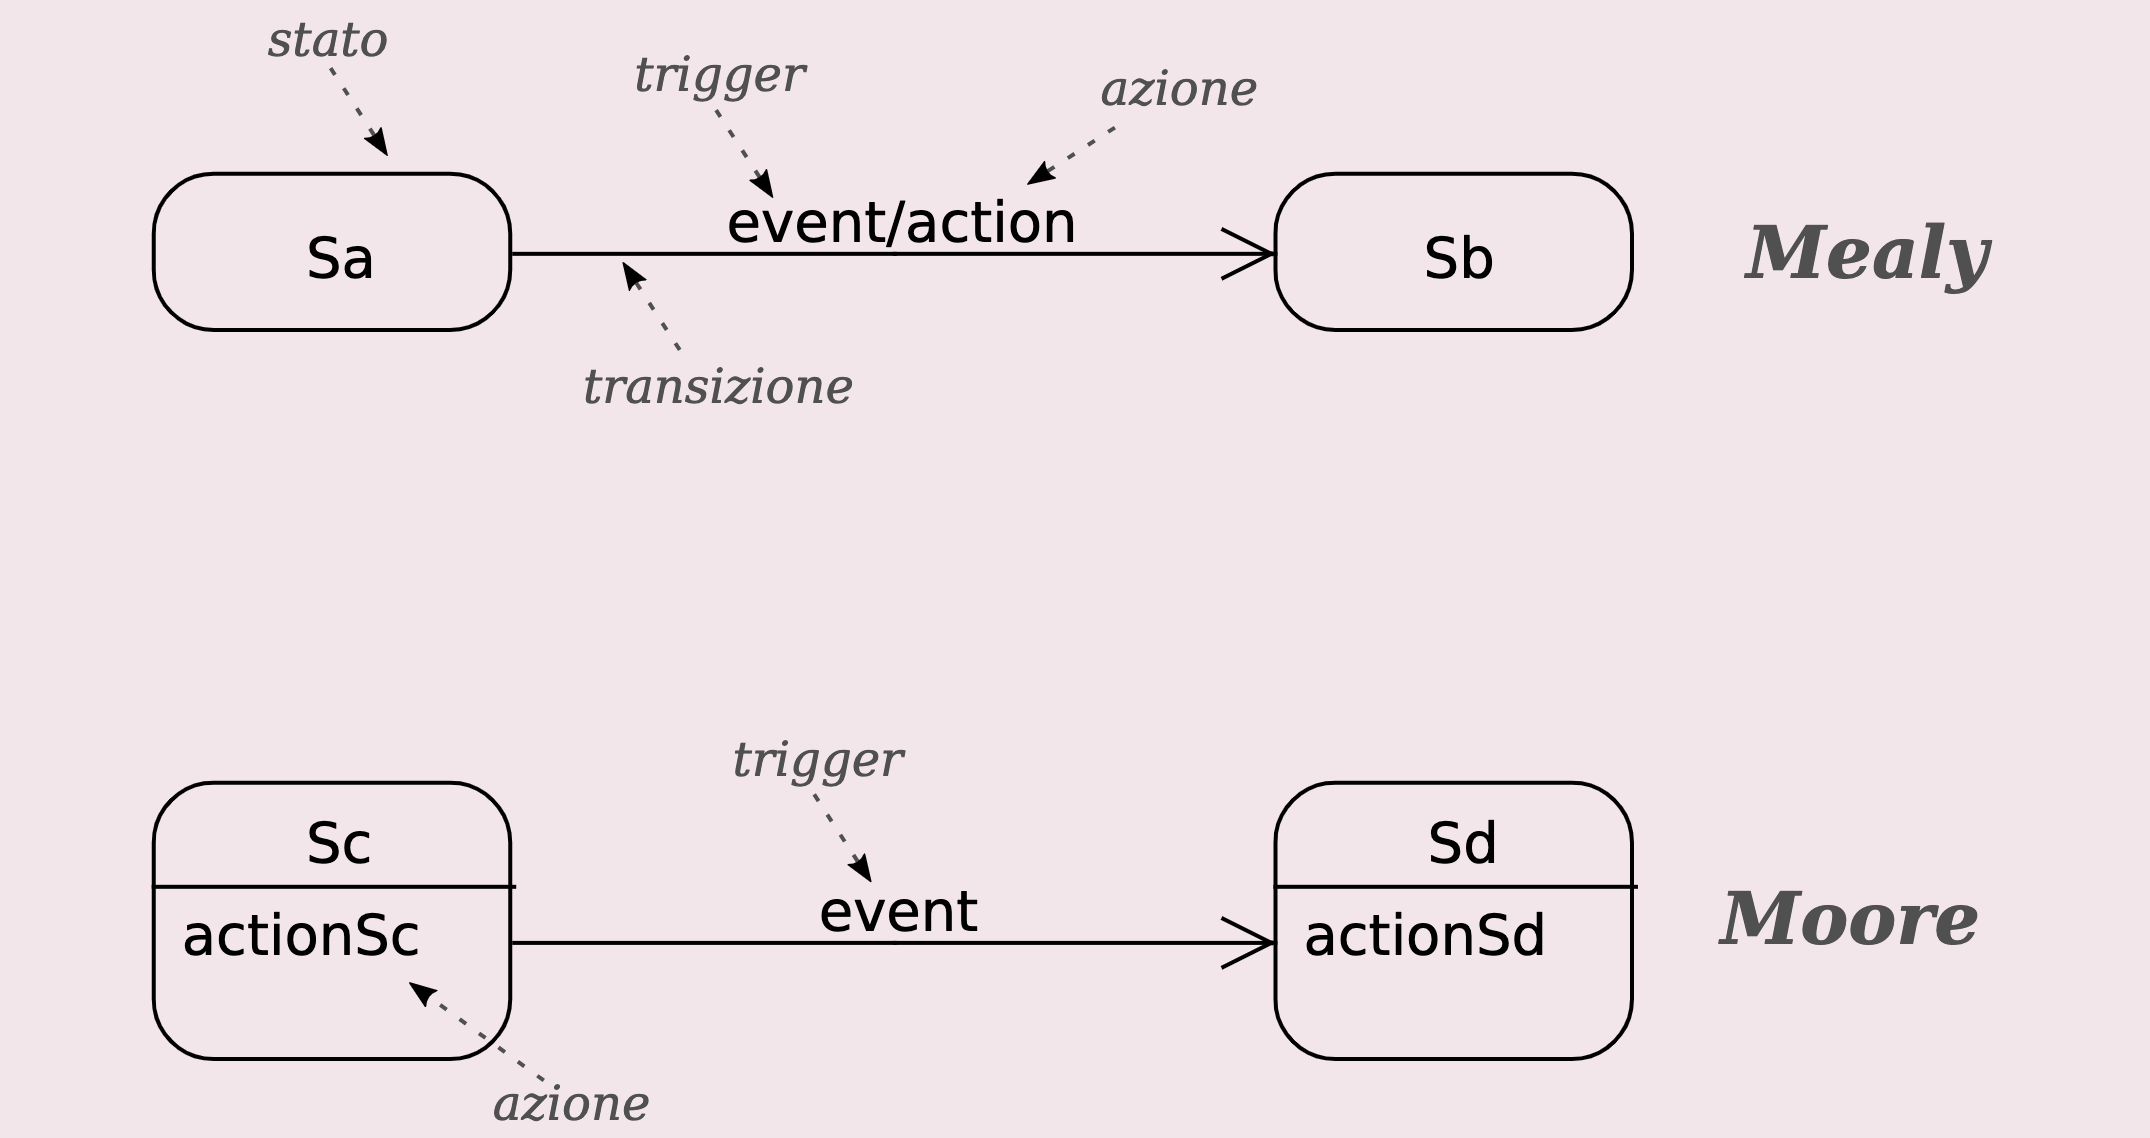
\includegraphics[width=0.75\linewidth]{assets/UML/state/state1.png}
\end{figure}

I due formalismi sono equivalenti: è sempre possibile trasformare un automa di Mealy in un automa di Moore e viceversa (il numero di stati potrebbe essere diverso).

\begin{figure}[H]
    \centering
    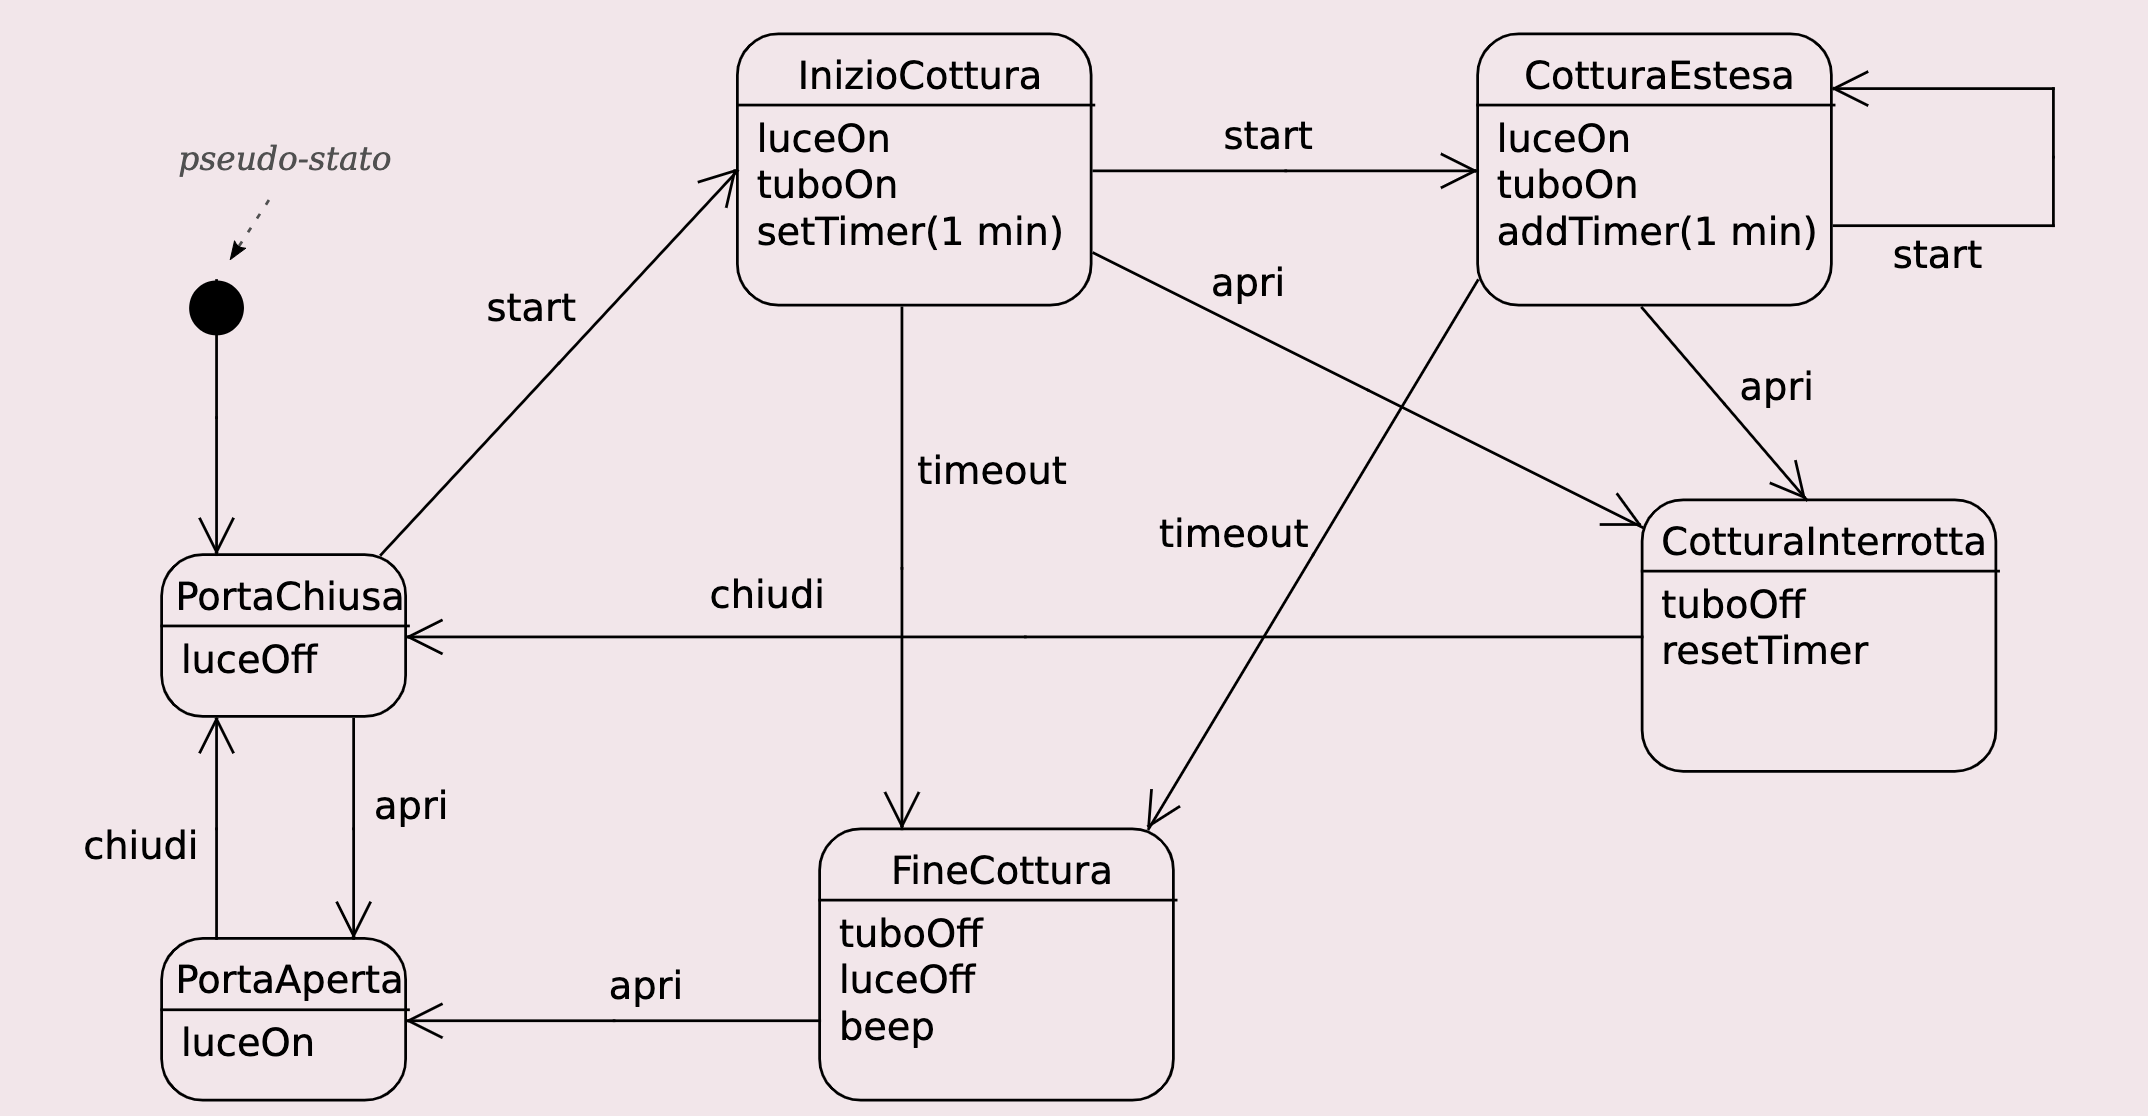
\includegraphics[width=0.75\linewidth]{assets/UML/state/state2.png}
    \caption{Esempio di automa: forno}
\end{figure}

\paragraph{State Chart} Sono una generalizzazione degli automi a stati finiti, rispetto ad essi consentono di modellare situazioni più complesse.

\begin{figure}[H]
    \centering
    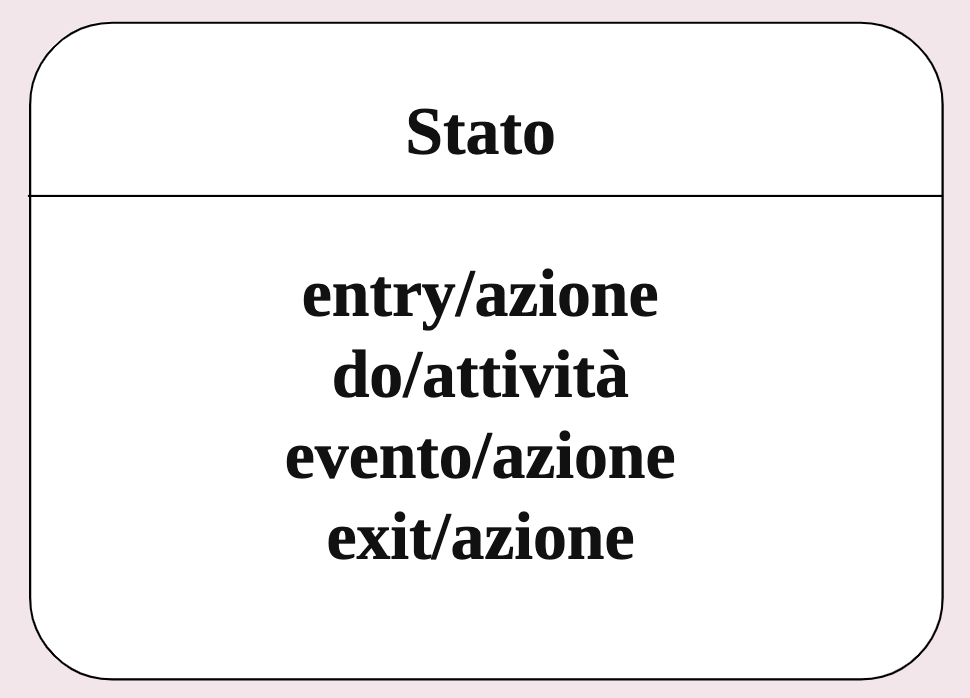
\includegraphics[width=0.25\linewidth]{assets/UML/state/state3.png}
    \caption{Rappresentazione di uno stato di controllo in uno state chart}
\end{figure}

\paragraph{Entry action} Azione triggerata entrando nello stato. Non va confusa con le \textit{attività interne} (non atomica, interrotta all'uscita dallo stato).

\paragraph{Exit action} Azione triggerata uscendo dallo stato. Si parla di \textit{transizione interna} quando l'oggetto esegue un'operazione rispetto ad un evento, ma senza uscire dallo stato. Si parla di \textit{transizione riflessiva} quando l'azione comporta il trigger di entrambe una entry action ed una exit action che riportano lo stato come era inizialmente (AUTOANELLO).

Gli state chart consentono di corredare i trigger con parametri e guardie (condizioni booleane in funzione dello stato corrente dell'oggetto e/o dei parametri ricevuti):

$$evento(parametro)\ \ [guardia]/azione$$

L'azione verrà eseguita se si verifica il trigger e se allo stesso tempo è vera la guardia. Fra le possibili azioni l'oggetto ha la facoltà di triggerare un altro oggetto (target).

$$send\ target.evento(parametri)$$

Scrivere dentro uno stato "evento/skip" specifica all'automa di ignorare il trigger quando si trova in quello stato.

Gli statechart consentono di modellare delle gerarchie annidando gli stati di controllo: ogni stato è contenuto in uno stato di livello gerarchico superiore (\textbf{\textit{superstato}}) che può a sua volta contenere più stati di livello gerarchico inferiore (\textbf{\textit{sottostati}}). Si dice \textbf{\textit{foglia}} uno stato privo di sottostati. Uno statechart in cui tutti gli stati sono sullo stesso piano gerarchico viene detto \textbf{\textit{piatto}}.

\begin{figure}[H]
    \centering
    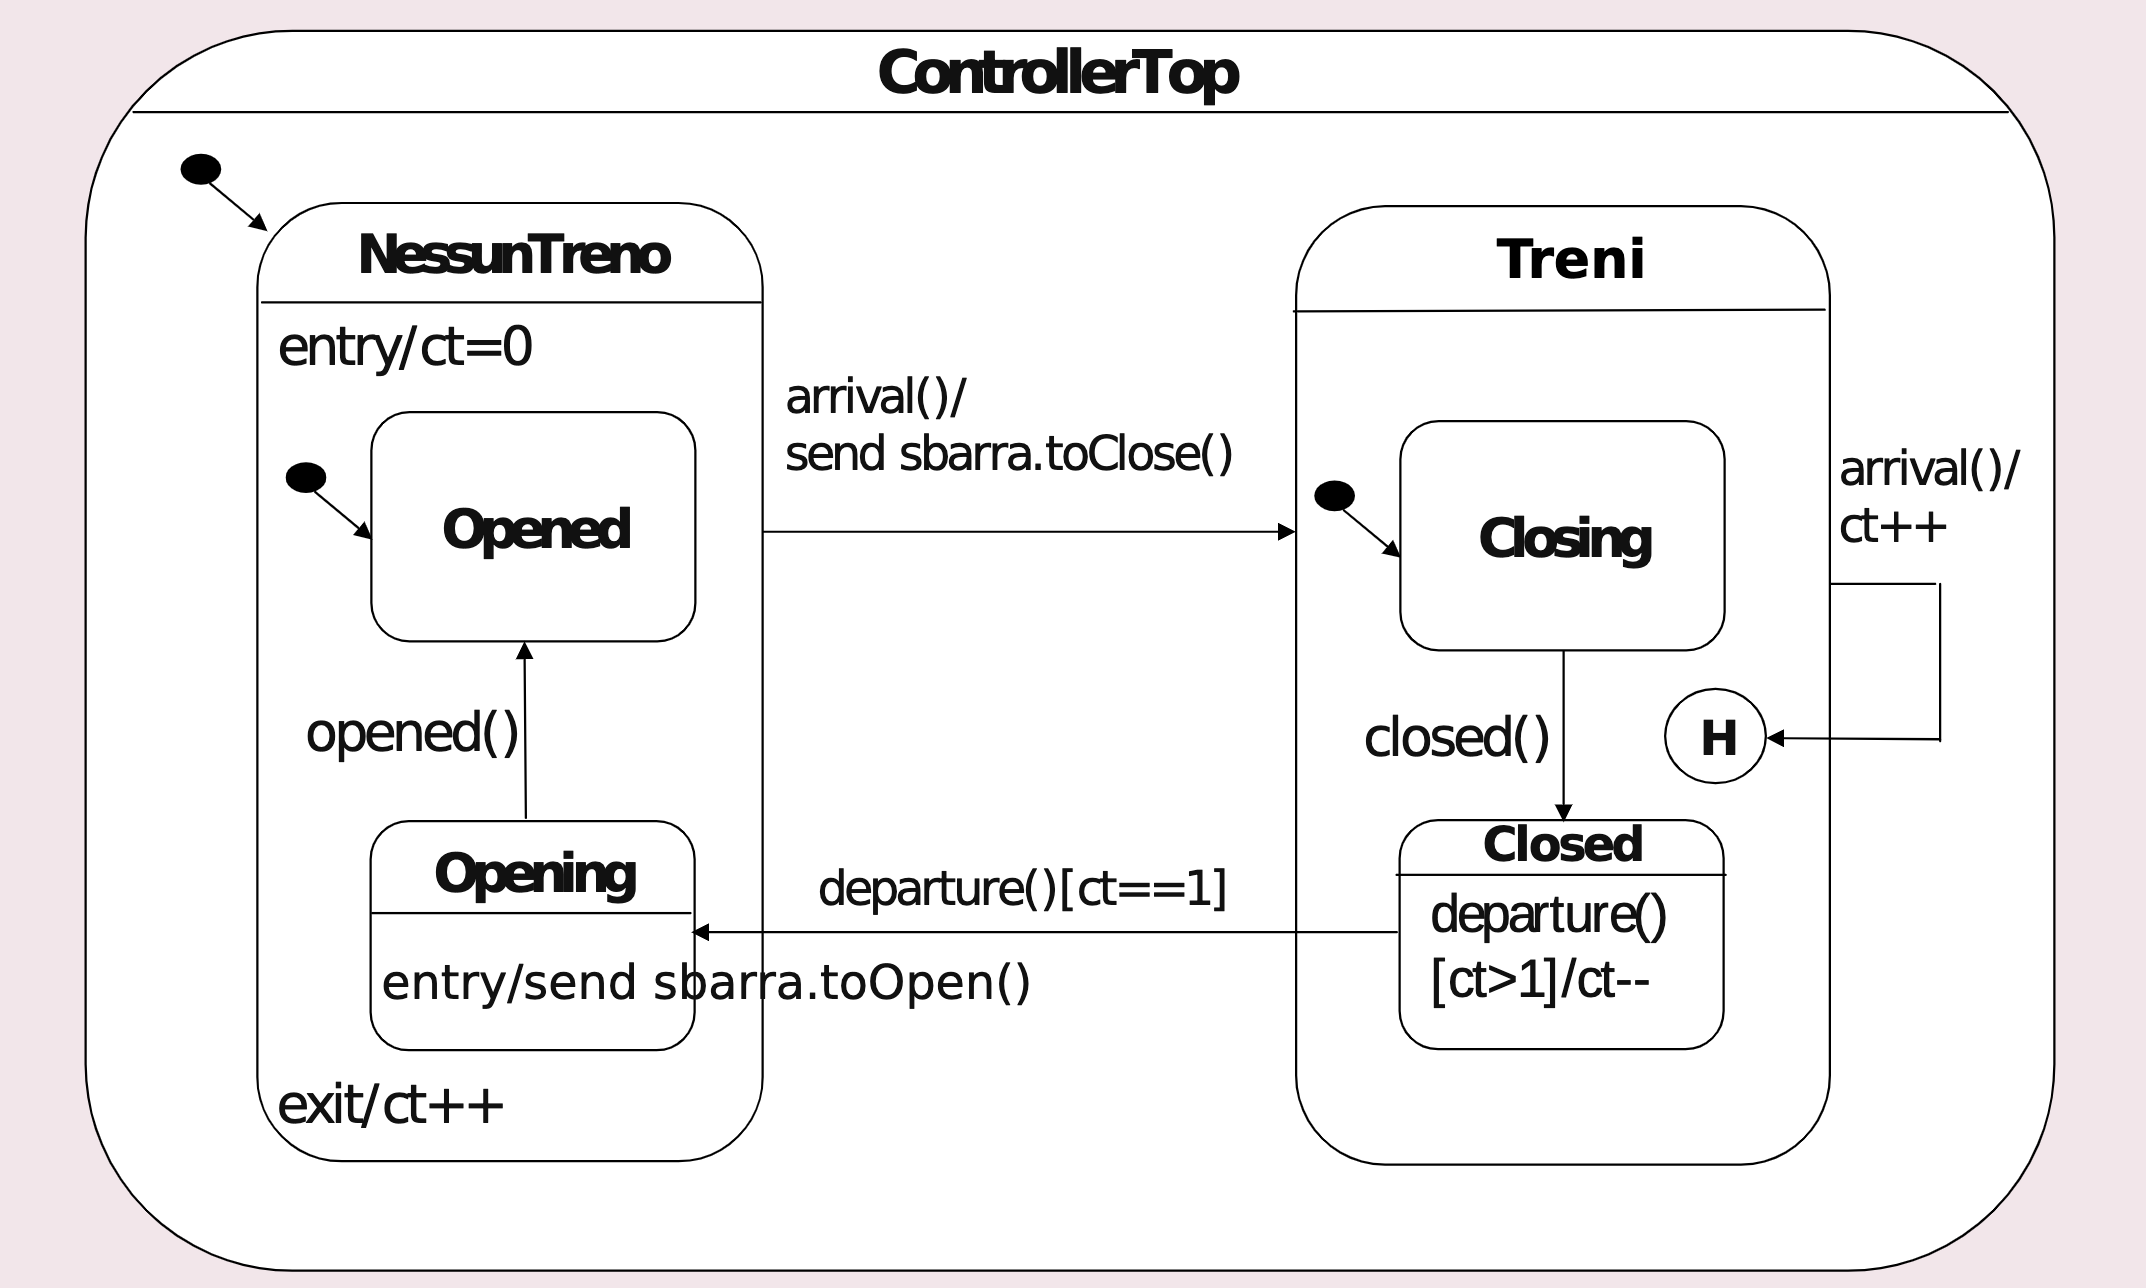
\includegraphics[width=0.75\linewidth]{assets/UML/state/state4.png}
    \caption{Esempio di state chart: controller di un treno}
\end{figure}

Per ogni stato non foglia una pseudo-transizione indica qual è il sottostato iniziale. Si definisce "configurazione" dell'automa il percorso che va dallo stato di più alto livello gerarchico fino allo stato foglia attuale. Nell'esempio, la configurazione iniziale dell'automa è la seguente:

$$ControllerTop.NessunTreno.0pened$$

\paragraph{OR-decomposition} Lo stato foglia attuale è sufficiente a definire univocamente la configurazione corrente dell'automa. Questo perché si è applicato il \textbf{principio dell'OR esclusivo} (XOR): in ogni stato NON foglia, l'automa deve trovarsi in uno e uno solo dei ossibili sottostati.

Si definisce \textbf{transizione di gruppo} quella che parte da uno stato non foglia: può essere triggerata a presciendere dal sottostato specifico in cui si trova l'automa. 

Un \textbf{connettore di storia} è un elemento posto all'interno di uno stato di controllo per consentire all'automa di memorizzare, quando si trova in quello stato, la configurazione corrente. Tornando nello stato l'automa non assumerà la configurazione di default, bensì quella memorizzata nel connettore. Esistono due tipi di connettori di storia:
\begin{itemize}
    \item \textbf{Storia superficiale (H)}: memorizzano la configurazione dallo stato di livello gerarchico più alto fino al livello dei sottostati dello stato con il connettore;
    \item \textbf{Storia profonda (H*)}: memorizzano la configurazione dallo stato di livello gerarchico più alto fino allo stato foglia corrente, dunque scendendo in profondità oltre i sottostati dello stato contenente il connettore.
\end{itemize}

\begin{figure}[H]
    \centering
    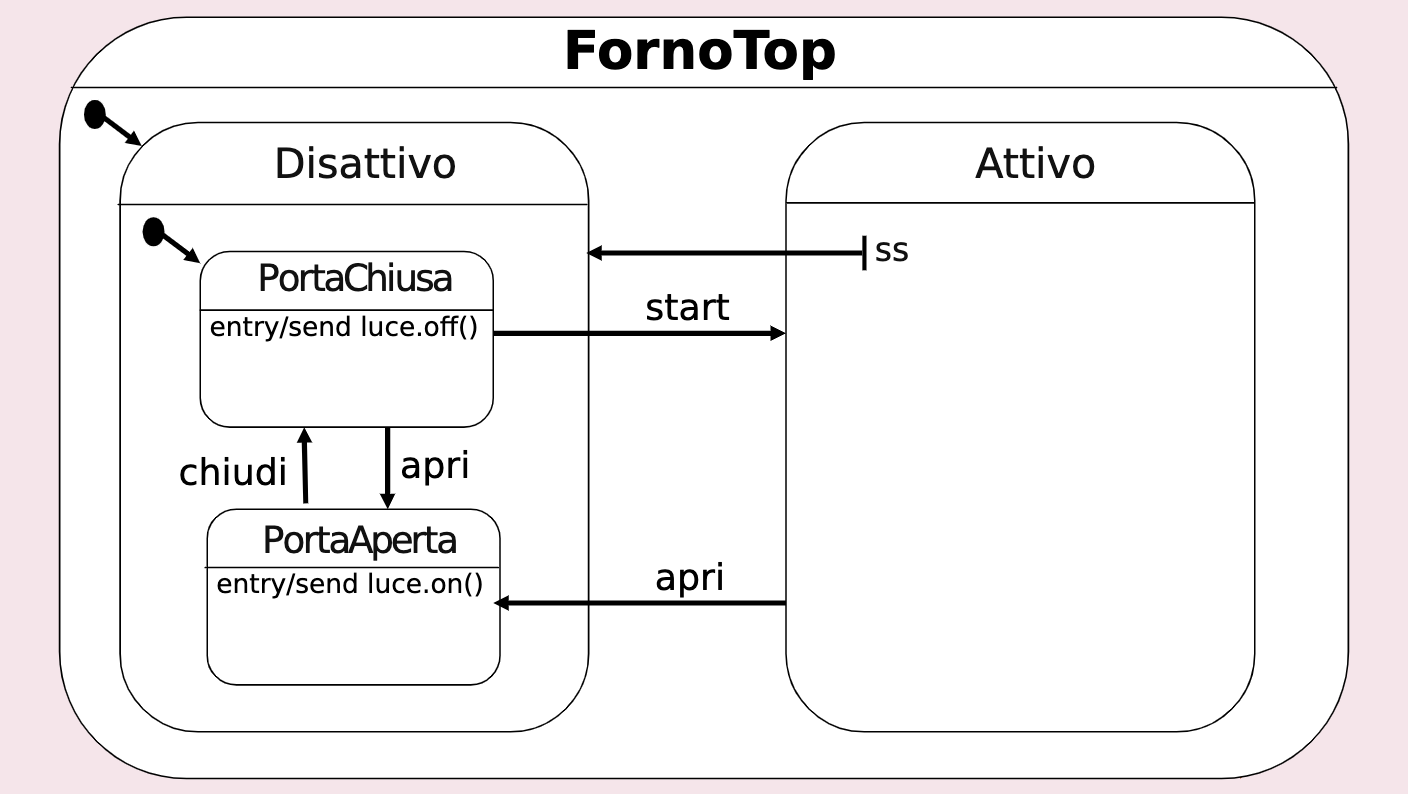
\includegraphics[width=0.75\linewidth]{assets/UML/state/state5.png}
    \caption{Esempio di statechart per il Forno}
\end{figure}

\begin{figure}[H]
    \centering
    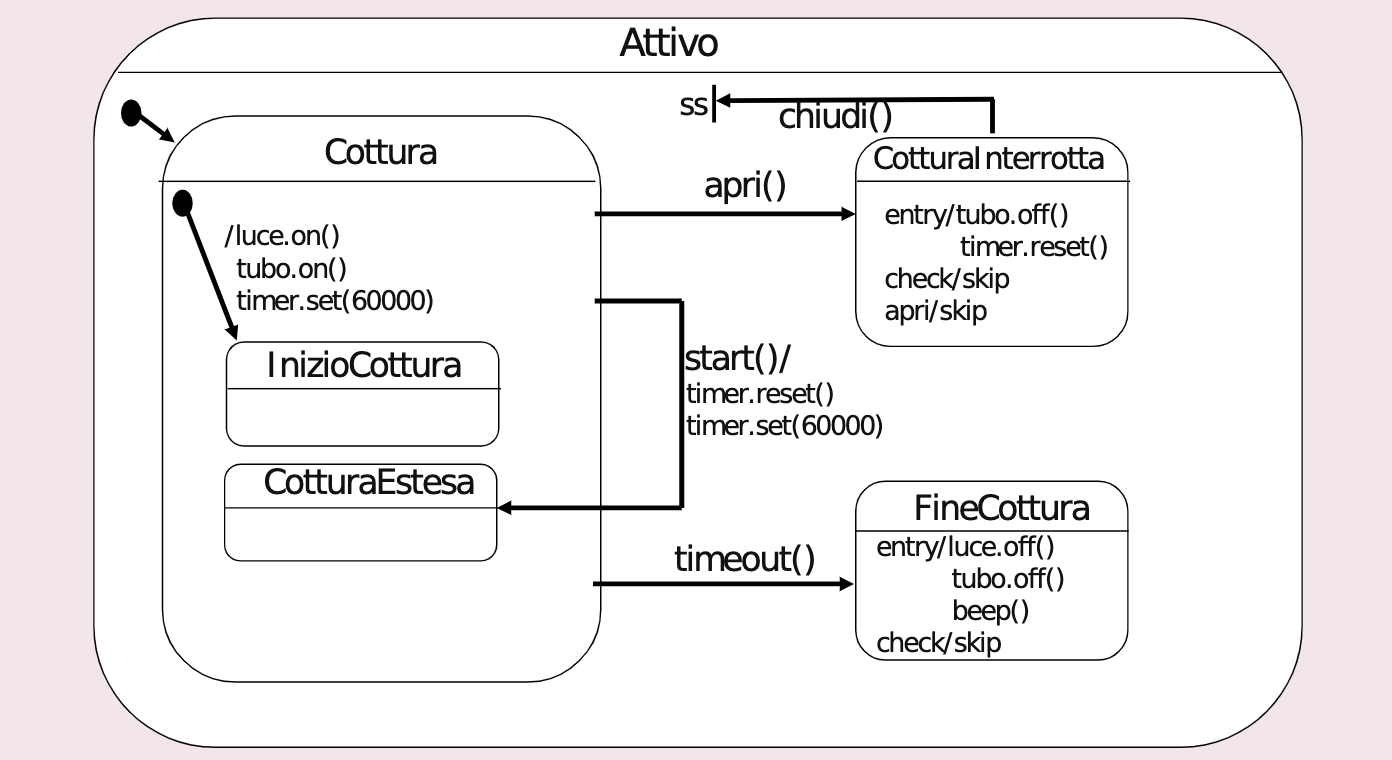
\includegraphics[width=0.75\linewidth]{assets/UML/state/state6.png}
    \caption{Definizione del macrostato "Attivo"}
\end{figure}

\begin{figure}[H]
    \centering
    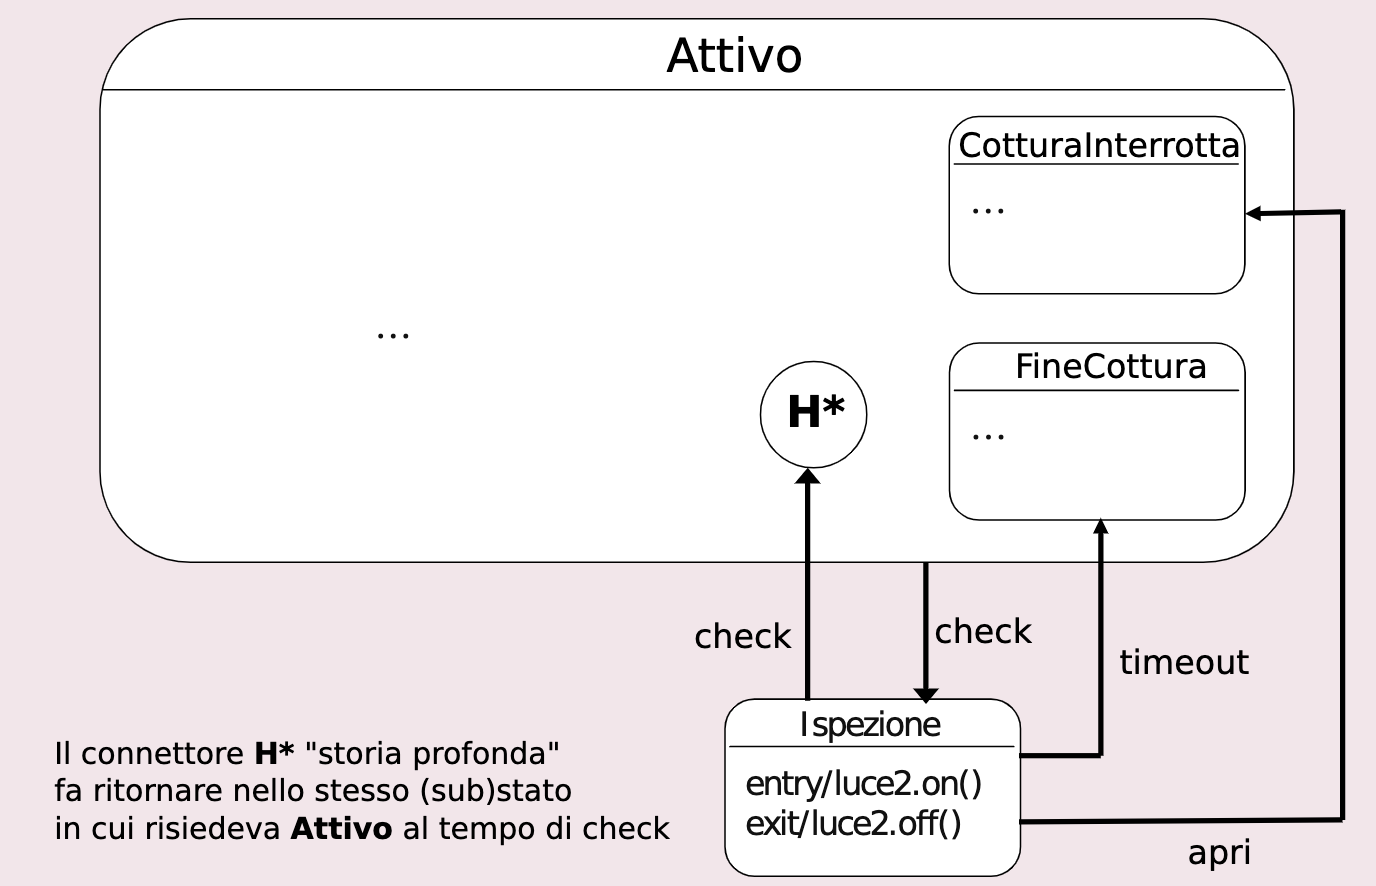
\includegraphics[width=0.75\linewidth]{assets/UML/state/state7.png}
    \caption{Esempio di stato ispezione}
\end{figure}

In generale i connettori di storia dovrebbero avere anche una transizione uscente verso un sottostato del macrostato in cui sono contenuti, in modo da poter essere attivati quando l'automa si trova in quello stato. In sua assenza e in assenza di memoria si raggiunge lo stato di default.

Sfruttando il principio di modularità, è possibile definire la gerarchia di uno solo dei possibili stati di controllo, astraendo dai dettagli interni degli altri stati. La presenza di stati non ancora definiti che sono punto di partenza/arrivo di transizioni è segnalata con un cosiddetto \textbf{state stub}.

\paragraph{Nota} Per via del concetto di configurazione, in una transizione di stato è necessario individuare:

\begin{itemize}
    \item \textbf{Exit path}: elenco degli stati di controllo da cui si esce, partendo dallo stato sorgente della transizione e risalendo fino al \textbf{Minimum Common Ancestor} (MCA) con lo stato di destinazione (MCA escluso). Si devono eseguire exit action di tutti gli stati attraversati.
    \item \textbf{Entry path}: elenco degli stati di controllo in cui si entra, partendo dall'MCA (escluso) e scendendo fino allo stato destinazione della transizione. Si devono eseguire tutte le entry action degli stati attraversati.
\end{itemize}

L'MCA è il superstato di livello gerarchico più piccolo che contenga sia la destinazione che la sorgente della transizione.

\subsubsection{Estendere lo state diagram}

Si possono includere negli statechart elementi tipici di un activity diagram: es. punti decisionali (rombi) che pongono due o più transizioni in alternativa. Si può introdurre un'attività (non atomica, interrompibile) in uno stato dcon la sintassi:

$$do:activity_name$$

Uno stato con una attività interna o con eventi processati localmente allo stato può essere scomposto in più sottostati. È possibile triggerare una transizione non con un evento esterno, bensì tramite la maturazione di una condizione internamente all'oggetto:

$$when condition$$

Ancora, il trigger della transizione potrebbe essere un \textit{evento di tempo}:

$$after time_expression$$


\paragraph{AND-decomposition} Lo stato foglia attuale NON è sufficiente a definire univocamente la condizione corrente dell'automa. In ogni stato NON foglia, l'automa può trovarsi contemporaneamente in due o più possibili sottostati. Lo stato viene diviso in \textit{regioni} parallele e concorrenti.

\begin{figure}[H]
    \centering
    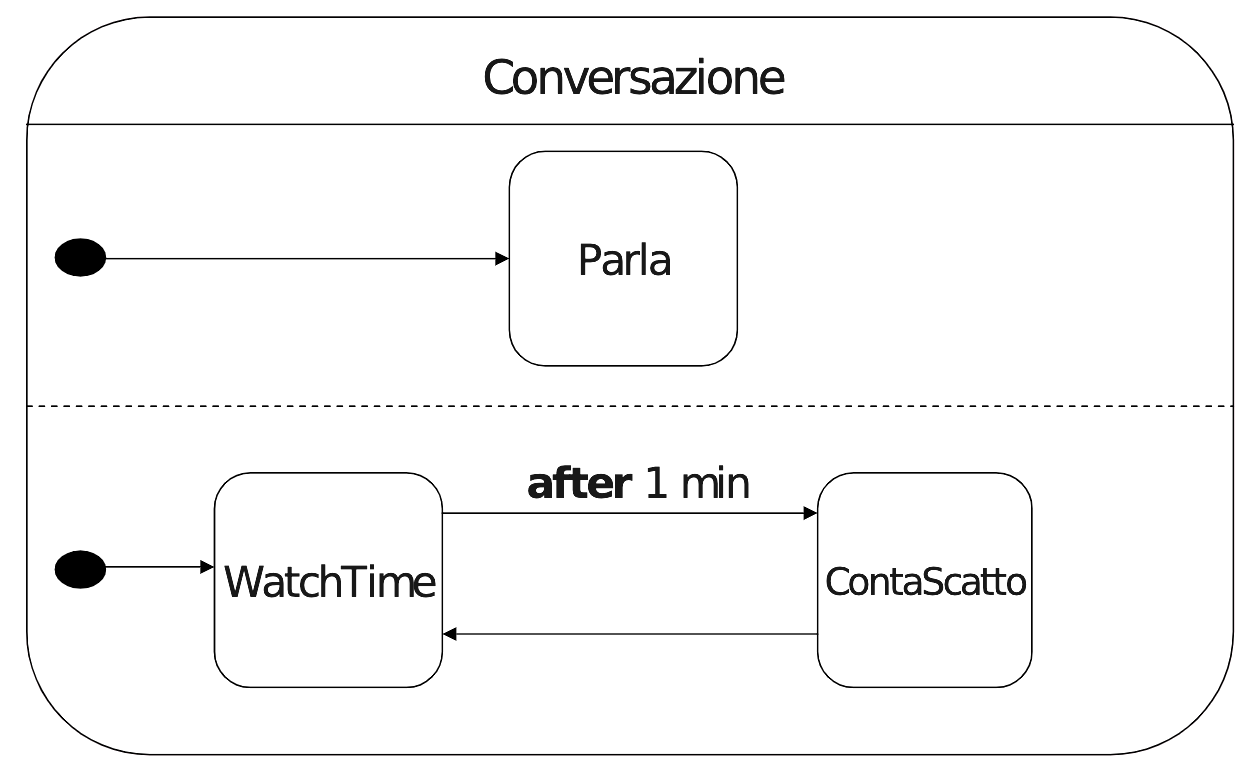
\includegraphics[width=0.75\linewidth]{assets/UML/state/state8.png}
\end{figure}

Nell'esempio, la configurazione inziale è:

$$Conversazione.Parla|WatchTime$$ 

Sottostati paralleli implicano l'esistenza di thread multipli in uno stesso oggetto (occorre adottare meccanismi di mutua esclusione per proteggere i dati condivisi).

Le transizioni nei due stati paralleli possono essere sincronizzate introducendo delle \textbf{barre di sincronizzazione} e degli \textbf{pseudo-stati di sincronismo} (synch state): l'avanzamento in un sottostato può awenire solo se nello stato parallelo si è raggiunto un certo punto.

\begin{figure}[H]
    \centering
    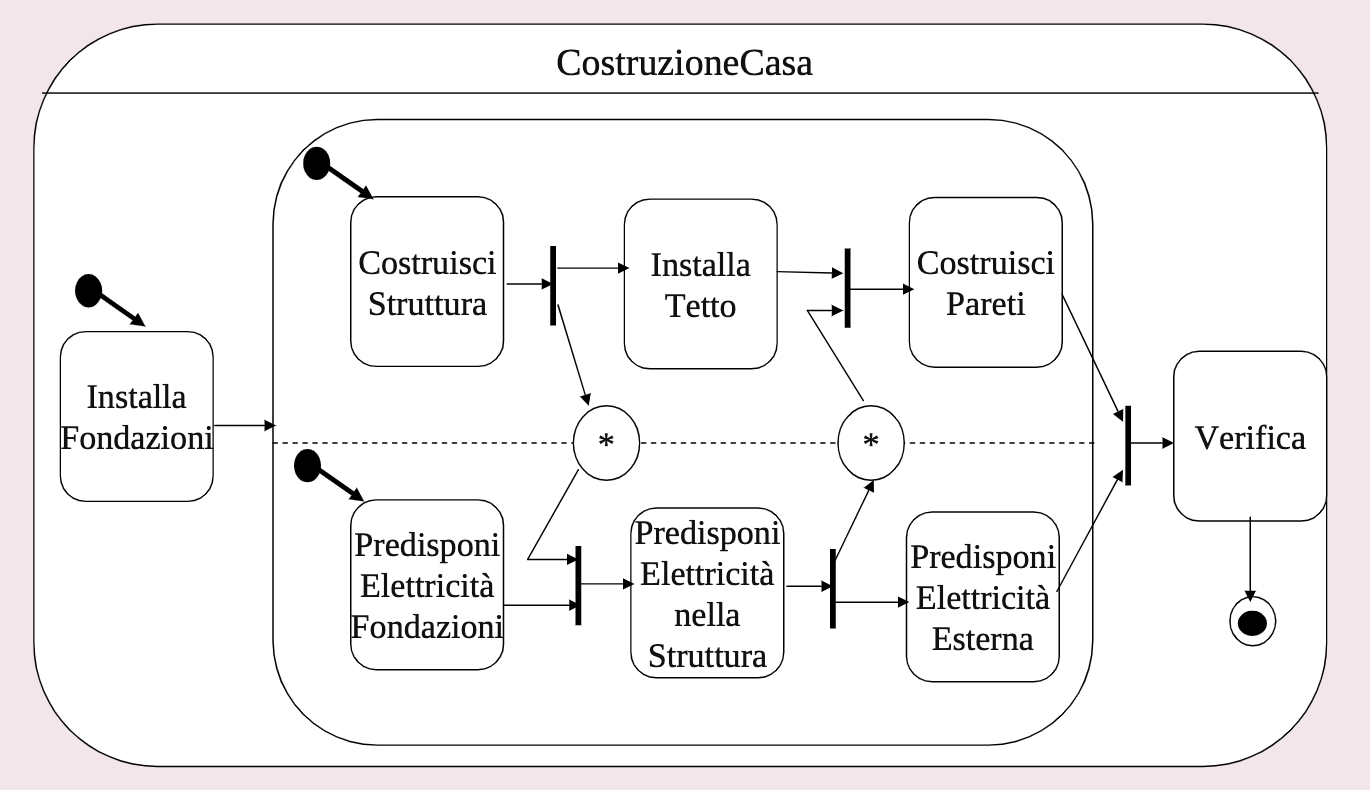
\includegraphics[width=0.75\linewidth]{assets/UML/state/state9.png}
\end{figure}

\newpage
\subsection{Structure Composite}

Lo \textbf{structure composite diagram} consente di scomporre gerarchicamente una classe sulla base dei suoi contenuti (interfacce richieste e fornite) e di mostrare la composizione interna delle sue istanze. Illustra le dipendenze dinamiche fra gli oggetti che compongono il sistema.

\begin{figure}[H]
    \centering
    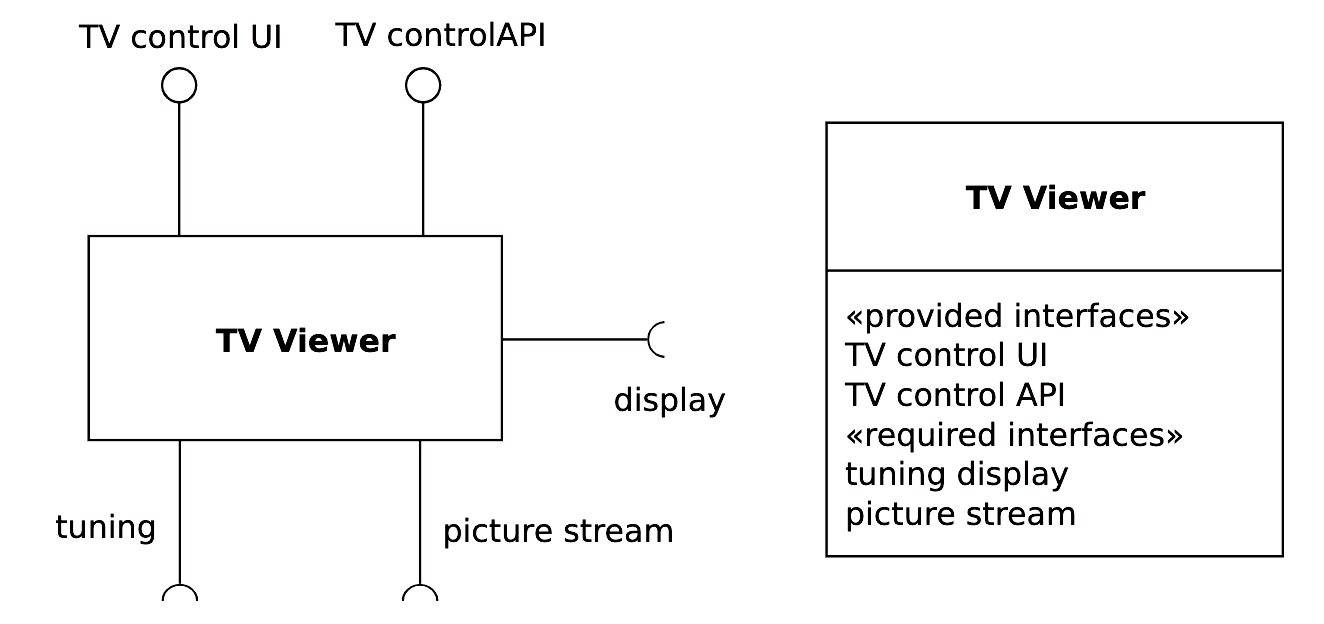
\includegraphics[width=0.75\linewidth]{assets/UML/struct_comp/struct_comp.png}
    \caption{Struttura interna della classe; le interfacce richieste/fornite sono raggruppate logicamente tramite "porte".}
\end{figure}

\paragraph{Esempio} TV Viewer: ogni istanza possiede un'istanza di TVPresenter e un'istanza di Generator (campi dell'oggetto), attraverso le quali fornisce e richiede determinate interfacce. Ogni proprietà posseduta dalla classe è una parte dell'istanza, indicata da \textbf{nome:classe} e dalla molteplicità. Le varie parti sono collegate da \textbf{connettori} (linee continue). I \textbf{connettori di delega} (frecce tratteggiate a punta aperta) collegano una parte alle interfacce che fornisce o richiede.

\begin{figure}[H]
    \centering
    \includegraphics[width=0.4\linewidth]{assets/UML/struct_comp/struct_comp2.png}
    \caption{Esempio di structure composite (TV Viewer)}
\end{figure}

\newpage
\subsection{UseCase}

Gli \textbf{UseCase Diagram} servono per identificare le funzionalità svolte dal sistema software. Queste devono essere assegnate ad oggetti/classi (\textbf{assegnazione di responsabilità}). Si parte dalle macro-funzionalità, raffinandole fino ad arrivare ad operazioni che non ammettono decomposizione. Eventuali ambiguità possono essere chiarite tramite \textit{Activity Diagram}. L'analisi dei casi d'uso può:
\begin{itemize}
    \item aiutare ad identificare gli oggetti
    \item definire i casi di test di moduli
    \item descrivere le dinamiche di interazione con il sistema
\end{itemize}

\begin{figure}[H]
    \centering
    \includegraphics[width=0.75\linewidth]{assets/UML/use-case/use-case1.png}
    \caption{Esempio di UseCase Diagram}
    \label{fig:use-case1}
\end{figure}

\paragraph{Attore} Rappresenta un ruolo interpretato da entità esterne (utenti o sistemi). L'\textbf{attore principale} è colui che persegue lo scopo del caso d'uso (gli altri sono secondari). Sussiste una relazione molti-a-molti tra attori e casi d'uso.

\textbf{\textit{Rappresentazione}}: omino stilizzato.

\paragraph{Scenario} Sequenza di passi che caratterizza l'interazione complessa tra un attore ed il sistema software stesso. In particolare si distinguono:
\begin{itemize}
    \item \textbf{Main scenario}: scenario principale di successo (obiettivo raggiunto)
    \item \textbf{Scenari secondari} (o estensioni del main): divergono dal main scenario o sono contenuti in esso (possono o meno raggiungere lo scopo prefissato)
\end{itemize}
\textbf{\textit{Rappresentazione}}: rettangolo contenente i casi d'uso dello scopo.

\paragraph{Caso d'uso} Insieme di scenari che hanno lo stesso scopo finale (per l'utente). Uno scenario è una possibile "esecuzione" (istanza) del caso d'uso. Può comprendere:
\begin{itemize}
    \item \textbf{Pre-condizioni}: descrivono ciò che il sistema deve assicurarsi prima che il caso d'uso possa avere inizio
    \item \textbf{Garanzie}: descrivono ciò che il sistema deve assicurarsi alla fine dello svolgimento del caso d'uso
    \item \textbf{Trigger}: specificano l'evento che da origine al caso d'uso
\end{itemize}
\textit{Alastair Cockburn} suddivide i casi d'uso in tre livelli:
\begin{itemize}
    \item \textbf{Kite-level}: mostrano come più sea-level portano all'interazione tra diversi attori (livello superficiale)
    \item \textbf{Sea-level}: interazioni attore principale/sistema (livello mediano)
    \item \textbf{Fish-level}: esistono perché inclusi in un sea-level (livello profondo)
\end{itemize}
Un passo di caso d'uso corrisponde ad un'interazione tra attore e sistema; è descritto da una frase semplice e non esprime dettagli tecnici.

\textbf{\textit{Rappresentazione}}: ellisse contenente il nome del caso d'uso.

\begin{figure}[H]
  \centering
  \subfloat[Generalizzazione tra casi d'uso, il caso d'uso figlio "specializza" (estende) alcuni aspetti del padre]{\includegraphics[width=0.575\linewidth]{assets/UML/use-case/use-case2.png}}
  \hfill
  \subfloat[Generalizzazione tra attori, ruolo figlio più specifico, \textit{compatibile} con il ruolo padre]{\includegraphics[width=0.25\linewidth]{assets/UML/use-case/use-case3.png}}
\end{figure}

\subparagraph{Estensione} Condizione che determina il verificarsi di interazioni diverse dallo scenario principale. Si indicano: il passo in cui si verifica la condizione, i passi (numerati) che descrivono le interazioni dell'estensione e (se necessario) il punto di rientro nello scenario principale.
\textbf{\textit{Rappresentazione}}: linea tratteggiata che termina con una freccia etichettata con la parola chiave $\langle\langle$extend$\rangle\rangle$

\begin{figure}[H]
  \centering
  \subfloat[Relazione di estensione]{\includegraphics[width=0.41\linewidth]{assets/UML/use-case/use-case5.png}}
  \hfill
  \subfloat[Esempio di caso d'uso in forma testuale]{\includegraphics[width=0.48\linewidth]{assets/UML/use-case/use-case4.png}}
\end{figure}

\subparagraph{Inclusione} Scissione di un passo di un caso d'uso complicato, espresso come un altro caso d'uso completo (il primo \textit{include} il secondo). In forma testuale è sufficiente sottolineare il nome del caso d'uso incluso.

\textbf{\textit{Rappresentazione}}: linea tratteggiata che termina con una freccia (dipendenza) etichettata con la parola chiave $\langle\langle$include$\rangle\rangle$

\newpage


\chapter{Design Pattern}

\section{Introduzione}

Un \textbf{Design Pattern} è una soluzione pronta all’uso o preliminarmente adattabile per specifici problemi applicativi. I Design Pattern affrontano questioni rilevanti come la riusabilità, la modificabilità, l’estendibilità e il disaccoppiamento dei moduli software. La loro conoscenza offre un linguaggio comune (sintassi e semantica) per facilitare la comunicazione all’interno dei team di progetto.

I Design Pattern si classificano in tre categorie principali:
\begin{itemize}
    \item \textbf{Creazionali}: si occupano della creazione degli oggetti.
    \item \textbf{Strutturali}: descrivono come comporre classi e oggetti.
    \item \textbf{Comportamentali}: si concentrano sulle interazioni tra oggetti e algoritmi.
\end{itemize}

Questa classificazione, sebbene ampiamente accettata, non è universalmente condivisa. Ad esempio, il pattern \textit{State} appartiene alla categoria comportamentale. I Design Pattern possono essere rappresentati tramite diagrammi UML che coinvolgono classi, interfacce, oggetti e le loro relazioni.

I \textbf{23 Design Pattern di riferimento} sono descritti nel libro \textit{Design Patterns: Elements of Reusable Object-Oriented Software} (Gang of Four: E. Gamma, R. Helm, R. Johnson, J. Vlissides, 1995). Tuttavia, nuovi pattern continuano a essere scoperti e documentati.

\subsection{Benefici dei Design Pattern}
L’uso dei Design Pattern facilita il riuso efficace di progetti e architetture, rendendo accessibili agli sviluppatori tecniche consolidate. Aiutano a scegliere tra alternative progettuali che migliorano la riusabilità del sistema e a scartare quelle che la comprometterebbero.

I Design Pattern rispondono a esigenze quali:
\begin{itemize}
    \item Isolare e incapsulare gli aspetti che cambiano in un progetto.
    \item Applicare il principio \textbf{Open/Closed}: apertura ai cambiamenti tramite l’aggiunta di nuovi moduli, mantenendo invariati gli altri.
    \item Migliorare la documentazione e la manutenzione dei sistemi esistenti.
\end{itemize}

\subsection{Struttura di un Design Pattern}
Ogni Design Pattern è caratterizzato da quattro elementi essenziali:
\begin{itemize}
    \item \textbf{Nome}: descrive sinteticamente il problema di progettazione, la soluzione e le conseguenze della soluzione scelta.
    \item \textbf{Problema (o intento)}: spiega il contesto e il problema che il pattern risolve.
    \item \textbf{Soluzione (concettuale)}: descrive gli elementi del progetto, le loro relazioni e collaborazioni. Non fornisce un’implementazione, ma una configurazione astratta.
    \item \textbf{Conseguenze}: descrivono i risultati e i vincoli derivanti dall’applicazione del pattern, aiutando a valutare soluzioni alternative e stimare costi e benefici.
\end{itemize}

\subsection{Origini dei Design Pattern}
Il concetto di pattern è stato introdotto da \textbf{Christopher Alexander} nel suo libro \textit{A Pattern Language: Towns, Buildings, Constructions} (Oxford University Press, 1977). Alexander descrisse circa 250 pattern per la progettazione architettonica di case e città, fornendo per ciascuno un nome, un contesto d’uso, il problema da risolvere e la soluzione proposta.

Un esempio di pattern architettonico è il \textit{Corridoio corto}, che suggerisce di evitare corridoi più lunghi di 16-17 metri per ridurre il disagio causato dalla loro oscurità e desolazione. La soluzione consiste nel progettare corridoi corti con ampie vetrate e rientranze arredate.

\subsection{Classificazione dei Design Pattern}
I Design Pattern possono essere classificati secondo due criteri:
\begin{itemize}
    \item \textbf{Scopo}: indica ciò che il pattern fa (Creazionali, Strutturali, Comportamentali).
    \item \textbf{Raggio d’azione}: distingue tra pattern che riguardano le relazioni statiche tra classi (\textit{Class-pattern}) e quelli che riguardano le relazioni dinamiche tra oggetti (\textit{Object-pattern}).
\end{itemize}

La maggior parte dei Design Pattern ha gli oggetti come raggio d’azione, ma alcuni si concentrano sulle classi. Ad esempio:
\begin{itemize}
    \item \textbf{Pattern Creazionali}: delegano parte del processo di creazione di un oggetto alle sottoclassi o ad altri oggetti.
    \item \textbf{Pattern Strutturali}: utilizzano l’ereditarietà per comporre classi o descrivono modi per raggruppare oggetti.
    \item \textbf{Pattern Comportamentali}: descrivono algoritmi e flussi di controllo o il modo in cui gruppi di oggetti cooperano per svolgere attività complesse.
\end{itemize}

\newpage

\section{Creazionali}

I pattern creazionali permettono di astrarre il processo di creazione. 
\begin{itemize}
    \item \textbf{Class Creational}: utilizzano l'ereditarietà per variare le classi istanziate \textit{(inheritance)};
    \item \textbf{Object Creational}: delegano il processo ad un altro oggetto \textit{(delegation or composition);}
\end{itemize}
Inoltre forniscono molta flessibilità su \textit{cosa} viene creato, \textit{chi} crea, \textit{come} viene creato e \textit{quando}.

\subsection{Abstract Factory}
\label{abstract-factory}

\textbf{Scopo}: Creazionale \\
\textbf{Raggio d'azione}: Oggetti

\paragraph{Definizione} Fornisce un’interfaccia per la creazione di famiglie di oggetti correlati o dipendenti senza specificare quali siano le loro classi concrete.

\paragraph{Problema} Si consideri lo sviluppo di un toolkit per la realizzazione di GUI in grado di supportare diversi look-and-feel. Affinché sia possibile il codice che la implementa non deve dipendere dal tipo specifico dei widget utilizzati quindi non può istanziarli direttamente.

\begin{figure}[H]
    \centering
    \includegraphics[width=1\linewidth]{assets/pattern/abstract-factory/abstract-factory-esempio.png}
\end{figure}

\paragraph{Soluzione} L’interfaccia WidgetFactory introduce un metodo per la creazione di ciascun tipo di base di widget definito a sua volta da un’oportuna interfaccia. I client invocano i metodi definiti da WidgetFactory per ottenere istanze di widget senza conoscere la classe concreta che utilizzano. Esiste una classe concreta che implementa WidgetFactory per ciascuno dei L\&F considerati.

\begin{figure}[H]
    \centering
    \includegraphics[width=1\linewidth]{assets/pattern/abstract-factory/abstract-factory-struttura.png}
    \caption{Class Diagram del pattern Abstract Factory}
\end{figure}

\paragraph{Struttura e Conseguenze} I partecipanti del pattern sono:
\begin{itemize}
    \item \textbf{AbstractFactory} (WidgetFactory): dichiara un’interfaccia per le operazioni di creazione di oggetti prodotto astratti.
    \item \textbf{ConcreteFactory} (MotifWidgetFactory, GtkWidgetFactory): implementa le operazioni degli oggetti prodotto concreti. 
    \item \textbf{AbstractProduct} (Window, ScrollBar): dichiara un’interfaccia per un tipo di prodotti
    \item \textbf{ConcreteProduct} (MotifWindow, GtkWindow): implementa l’interfaccia Product definendo un oggetto prodotto creato dalla corrispondente factory concreta.
\end{itemize}

Il pattern AbstractFactory consente quindi di isolare le classi concrete (processo di creazione incapsulato nella Factory), cambiare agilmente la famiglia di prodotti utilizzata (cambio di configurazione cambiando il tipo di Factory) e promuovere la coerenza nell'utilizzo dei prodotti.

È bene notare che l'aggiunta del supporto a nuove tipologie di prodotti è difficile in quanto comporta la modifica dell'interfaccia AbstractFactory e, di conseguenza, di tutte le classi che la implementano.

In più è possibile implementare il Factory come Singleton (\ref{singleton})

\begin{figure}[H]
    \centering
    \includegraphics[width=1\linewidth]{assets/pattern/abstract-factory/abstract-factory-sequence.drawio.png}
    \caption{Sequence Diagram del pattern Abstract Factory}
\end{figure}

\newpage
\subsection{Builder}
\label{builder}

\textbf{Scopo}: Creazionale \\
\textbf{Raggio d'azione}: Oggetti

\paragraph{Definizione} Il patter Builder permette di separare la costruzione di un oggetto complesso dalla sua rappresentazione, in modo che lo stesso processo di costruzione possa essere utilizzato per creare rappresentazioni diverse.

\paragraph{Problema} Prendiamo in considerazione un’applicazione capace di leggere documenti in formato RTF che può supportare la conversione in altri formati (ASCII, LaTeX).

\begin{figure}[H]
    \centering
    \includegraphics[width=1\linewidth]{assets/pattern/builder/builder-esempio.png}
\end{figure}

\paragraph{Soluzione} Una soluzione consiste nel configurare la classe RTFReader con un oggetto conforme all’interfaccia TextConverter in grado di gestire la conversione in un altro formato. Il documento nel formato di uscita viene costruito man mano che gli elementi del documento RTF sono analizzati.

\begin{figure}[H]
    \centering
    \includegraphics[width=1\linewidth]{assets/pattern/builder/builder-struttura.png}
\end{figure}

\paragraph{Struttura e Conseguenze} Il pattern è composto da:
\begin{itemize}
    \item \textbf{BuilderIF}: specifica l’interfaccia astratta che crea le parti dell’oggetto Product. 
    \item \textbf{ConcreteBuilder}: costruisce e assembla le parti del prodotto implementando l’interfaccia Builder; definisce e tiene traccia della rappresentazione che crea.
    \item \textbf{Director}: costruisce un oggetto utilizzando l’interfaccia Builder.
    \item \textbf{Product}: rappresenta l’oggetto complesso e include le classi che definiscono le parti che lo compongono, includendo le interfacce per assemblare le parti nel risultato finale.
\end{itemize}

Permette quindi di: variare la rappresentazione interna di un prodotto, isolare il codice per la costruzione la rappresentazione e consente di avere maggiore controllo del processo di costruzione.

Risolve allo stesso tempo il problema dei \textbf{costruttori telescopici}, e si propone come alternativa a tecnologie come JavaBeans.

\newpage

\textbf{Esempio Java}

\begin{minted}[
    fontsize=\footnotesize,
    linenos,
]{java}
public class NutritionFacts { 

    private final int servingSize; 
    private final int servings; 
    private final int calories ; 
    private final int fat ; 
    private final int sodium; 
    private final int carbohydrate; 
    
    public static class Builder { 
        // Required parameters 
        private final int servingSize; 
        private final int servings; 
        
        // Optional 
        private int calories = 0; 
        private int fat = 0; 
        private int carbohydrate = 0; 
        private int sodium = 0; 
        
        public Builder( int servingSize, int servings) { 
            this.servingSize = servingSize; 
            this.servings = servings; 
        } 
        
        public Builder calories ( int val ) { 
            calories = val ; return this;
        } 
        
        public Builder fat ( int val ) { 
            fat = val ; 
            return this; 
        } 
        
        public Builder carbohydrate(int val ) {
            carbohydrate = val; 
            return this; 
        } 
        
        public Builder sodium(int val) { 
            sodium = val; 
            return this; 
        } 
        
        public NutritionFacts build () { 
            return new NutritionFacts(this); 
        } 
    }
    
    private NutritionFacts (Builder builder ) { 
        servingSize = builder.servingSize; 
        servings = builder.servings; 
        calories = builder.calories; 
        fat = builder.fat;
        sodium = builder.sodium; 
        carbohydrate = builder.carbohydrate;
    }
}

// Utilizzo:
NutritionFacts cocaCola = new NutritionFacts.Builder(240, 8)
                            .calories(100)
                            .sodium(35)
                            .carbohydrate(27)
                            .build();

\end{minted}

\paragraph{Interazioni} L'utilizzo del pattern consiste nel creare un oggetto Director e configurarlo tramite l'oggetto Builder. Il Director informa il Builder ogni volta che una parte di Product deve essere costruita. Il Builder riceve e gestisce le richieste dal Director e aggiunge le parti al Product. Il client ottiene dal Builder il Product creato.

\begin{figure}[H]
    \centering
    \includegraphics[width=1\linewidth]{assets/pattern/builder/builder-sequence.drawio.png}
\end{figure}

\newpage
\subsection{Factory Method (\textit{o Virtual Constructor})}
\label{factory-method}

\textbf{Scopo}: Creazionale  \\
\textbf{Raggio d'azione}: Classi

\paragraph{Definizione} Definisce un'interfaccia per la creazione di un oggetto, lasciando alle sottoclassi la decisione sulla classe concreta che sarà istanziata. Consente di deferire la creazione di un oggetto alle sottoclassi.

\paragraph{Problema} Si consideri un framework per applicazioni in grado di presentare più documenti agli utenti.

\begin{figure}[H]
    \centering
    \includegraphics[width=1\linewidth]{assets/pattern/factory-method/factory-method-esempio.png}
\end{figure}

\paragraph{Soluzione} La classe Application è responsabile della gestione di oggetti conformi all’interfaccia Document e della loro creazione. Application sa solo quando dovrà creare un nuovo documento ma non di che tipo né come dovrà farlo. La responsabilità è spostata all’esterno del framework: le sottoclassi di Application devono fornire l’implementazione del metodo factory \textit{createDocument()} in modo da restituire un’istanza della classe appropriata

\paragraph{Struttura e Conseguenze} Il pattern è composto da:
\begin{itemize}
    \item \textbf{Product} (Document): definisce l'interfaccia degli oggetti creati dal metodo factory;
    \item \textbf{ConcreteProduct} (MyDocument): implementa l'interfaccia Product;
    \item \textbf{Creator} (Application): dichiara il metodo factory che restituisce un oggetto di tipo Product. Può invocare \textit{createProduct()} per creare un prodotto;
    \item \textbf{ConcreteCreator} (MyApplication): sovrascrive \textit{createProduct()} in modo da restituire una specifica istanza di ConcreteProduct;
\end{itemize}


\begin{figure}[H]
    \centering
    \includegraphics[width=1\linewidth]{assets/pattern/factory-method/factory-method-struttura.png}
    \caption{Class Diagram del pattern Factory Method}
\end{figure}

\begin{itemize}
    \item Elimina la necessità di riferirsi a classi dipendenti dall’applicazione all’interno del codice del framework.
    \item Gli utilizzatori potrebbero essere costretti a definire sottoclassi di Creator per creare un particolare oggetto ConcreteProduct.
    \item Fornisce un punto d’aggancio per le sottoclassi per la produzione di una versione specializzata di un prodotto.
    \item Connette gerarchie di classi parallele. Il metodo factory potrebbe invocato da oggetti diversi dal Creator.
\end{itemize}

\begin{figure}[H]
    \centering
    \includegraphics[width=0.8\linewidth]{assets/pattern/factory-method/factory-method-parallelo.png}
    \caption{Gerarchie di classi parallele}
\end{figure}

\begin{figure}[H]
    \centering
    \includegraphics[width=0.8\linewidth]{assets/pattern/factory-method/factory-method-sequence.drawio.png}
    \caption{Sequence Diagram del pattern Factory Method}
\end{figure}

\newpage
\subsection{Prototype}
\label{prototype}

\textbf{Scopo}: Creazionale \\
\textbf{Raggio d'azione}: Oggetti

\paragraph{Definizione} Specifica la tipologia di oggetti da creare utilizzando un'istanza prototipo e creare nuovi oggetti clonando questo prototipo.

\paragraph{Problema} Si pensi ad applicazione che consenta rappresentare degli elementi grafici nel piano cartesiano. L’applicazione potrebbe avere una barra di tasti per effettuare varie operazioni. Un’azione tipica è quella di creare un nuovo oggetto grafico. Per inserire differenti oggetti l’azione da compiere e` identica a parte il tipo di oggetto da creare.

\paragraph{Soluzione} Una soluzione consiste nel configurare l’oggetto responsabile della creazione (il tasto) con un prototipo dell’oggetto da creare.

\begin{figure}[H]
    \centering
    \includegraphics[width=0.75\linewidth]{assets/pattern/prototype/prototype-struttura.png}
    \caption{Class Diagram del pattern Prototype}
\end{figure}

\paragraph{Struttura e Conseguenze} Il pattern è composto da:
\begin{itemize}
    \item \textbf{Prototype}: specifica l'interfaccia che consente la clonazione
    \item \textbf{ConcretePrototype}: implementa l'operazione di clonazione
    \item \textbf{Client}: crea un nuovo oggetto chiedendo ad un prototipo di clonarsi
\end{itemize}

Condivide molte delle conseguenze di Abstract Factory (\ref{abstract-factory}) e Builder (\ref{builder}): nasconde le classi dei prodotti concreti, riducendo il numero di classi che devono essere note al client. In più:
\begin{itemize}
    \item Consente di aggiungere e rimuovere prodotti durante l’esecuzione;
    \item Consente la specifica di nuovi oggetti variando i valori;
    \item Consente la specifica di nuovi oggetti variando la struttura;
    \item Riduce il numero di sottoclassi
    \item Obbliga l'implementazione dell’operazione \textit{clone()}
\end{itemize}

\textbf{In Java}
Utilizzo dell'interfaccia \textit{Cloneable}, è possibile clonare oggetti in modo superficiale (shallow copy) o in maniera profonda (deep copy) ridefinendo il metodo clone().

\begin{minted}[
    fontsize=\footnotesize,
    linenos,
]{java}
// Shallow copy
public class Point2D implements Cloneable {
    private double x; 
    private double y;
    
    @Override public Point2D clone() { 
        try { 
            Point2D clone = (Point2D) super.clone(); 
            return clone;
        } catch (CloneNotSupportedException e) {
            throw new Error(e);
        } 
    } 
}
\end{minted}

\newpage

\begin{minted}[
    fontsize=\footnotesize,
    linenos,
]{java}

// Deep copy
public abstract class PolinomioAstratto implements Polinomio, Cloneable { 
    protected abstract PolinomioAstratto getPrototype(); 

    @Override public Polinomio add(Polinomio p) { 
        // crea un nuovo polinomio 
        Polinomio somma = getPrototype().clone(); 

        // aggiunge ciascun monomio di this al polinomio somma 
        for (Monomio m : this) somma.add(m); 
        
        // aggiunge ciascun monomio di p al polinomio somma 
        for (Monomio m : p) somma.add(m); 
        
        return somma; 
    } 
    
    @Override public PolinomioAstratto clone() { 
        try { 
            return (PolinomioAstratto) super.clone(); 
        } catch (CloneNotSupportedException e) { 
            throw new Error(e); 
        }
    }
}

public class PolinomioLL extends PolinomioAstratto { 
    private static PolinomioLL prototype; 
    private LinkedList<Monomio> monomi = new LinkedList<>(); 
    
    @Override protected synchronized PolinomioLL getPrototype() { 
        if ( prototype==null ) prototype = new PolinomioLL(); 
        return prototype;
    } 
    
    @Override public PolinomioLL clone() {
        PolinomioLL p = (PolinomioLL) super.clone();
        p.monomi = new LinkedList<Monomio>(); 
        for (Monomio m : this) p.monomi.add(m); 
        return p;
    }
}

\end{minted}

\newpage
\subsection{Singleton}
\label{singleton}

\textbf{Scopo}: Creazionale \\
\textbf{Raggio d'azione}: Oggetti

\paragraph{Definizione} Il pattern Singleton assicura che un classe abbia una sola istanza e fornisca un solo punto di accesso globale a tale istanza.

\paragraph{Problema} In un sistema potrebbero esistere più stampanti, ma potrebbe essere presente soltanto una coda di stampa. In un sistema operativo dovrebbe essere presente solo un file system e un solo window manager

\paragraph{Soluzione} Per assicurare che una classe abbia una sola istanza e che tale istanza sia facilmente accessibile per gli utilizzatori si può fare in modo che la classe stessa abbia la responsabilità di creare le proprie istanze. La classe può assicurare che nessun’altra istanza possa essere creata e può fornire un modo semplice per accedere all’istanza.

\begin{figure}[H]
    \centering
    \includegraphics[width=0.4\linewidth]{assets/pattern/singleton/singleton-struttura.png}
    \caption{Class Diagram del pattern Singleton}
\end{figure}

\paragraph{Struttura e Conseguenze} Il pattern risulta essere applicabile in due casi in particolare:
\begin{itemize}
    \item Quando deve esistere esattamente un’istanza di una classe resa accessibile ai client attraverso un punto di accesso noto a tutti gli utilizzatori.
    \item Quando l’unica istanza deve poter essere estesa attraverso la definizione di sottoclassi ed i client devono essere in grado di utilizzare le istanze estese senza dover modificare il proprio codice.
\end{itemize}

\textbf{Java}

\begin{minted}[
    fontsize=\footnotesize,
    linenos,
]{java}
public final class Singleton { 
    private static Singleton INSTANCE = null; 
    
    private Singleton(){} 
    
    public static synchronized Singleton getInstance() { 
        if (INSTANCE == null) { 
            INSTANCE=new Singleton(); 
        } 
        return INSTANCE; 
    } 
}
\end{minted}

\newpage

\section{Strutturali}

I pattern strutturali si occupano di come classi e oggetti sono composti per formare strutture più grandi. 
\begin{itemize}
    \item \textbf{Class Structural}: usano l'ereditarietà per definire interfacce o implementazioni;
    \item \textbf{Object Structural}: descrivono modi per comporre oggetti per realizzare nuove funzionalità
\end{itemize}

È bene sottolineare che alcuni pattern fanno utilizzo di ereditarietà multipla, non sempre applicabile in linguaggi come Java, che permettono di implementare molteplici interfacce, ma estendere una sola classe (astratta o concreta).

\subsection{Adapter (\textit{o Wrapper})}
\label{adapter}

\textbf{Scopo}: Strutturale \\
\textbf{Raggio d'azione}: Classi, Oggetti

\paragraph{Definizione} Permette di convertire l'interfaccia di una classe in un'altra interfaccia richiesta dal client.Consente a classi diverse di cooperare quando ciò non sarebbe possibile a causa di interfacce incompatibili.

\paragraph{Motivazione} A volte una classe preesistente, progettata per essere riutilizzata, non può essere riusata perché incompatibile con l'interfaccia richiesta dall'applicazione. Nell’esempio, la classe XXXTriangle non può essere riusata dove ci si aspetta l’interfaccia Figure2D perché non è compatibile con essa.

\begin{multicols}{2}
\begin{figure}[H]
    \centering
    \includegraphics[width=1\linewidth]{assets/pattern/adapter/adapter-esempio-class.png}
    \caption{Esempio di Class Adapter}
\end{figure}
\columnbreak
\begin{figure}[H]
    \centering
    \includegraphics[width=1\linewidth]{assets/pattern/adapter/adapter-esempio-object.png}
    \caption{Esempio di Object Adapter}
\end{figure}
\end{multicols}

Pensare di modificare XXXTriangle per renderla conforme a Figure2D non è una buona soluzione (si legherebbe al contesto specifico e il codice sorgente potrebbe non essere disponibile).

Si introduce una classe Triangle che sia al contempo erede di entrabe XXXTriangle e Figure2D. L'implementazione dei metodi di Figure2D sfrutta quelli di XXXTriangle.

È possibile introdurre la classe Triangle anche di modo che faccia riferimento ad un oggetto (istanza di XXXTriangle) e vada ad implementare l'interfaccia Figure2D delegando l'esecuzione all'oggetto incapsulato.

\begin{figure}[H]
    \centering
    \includegraphics[width=0.75\linewidth]{assets/pattern/adapter/adapter-sequence.drawio.png}
    \caption{Sequence diagram raggio d'azione}
\end{figure}

\paragraph{Applicabilità} È consigliabile utilizzare il pattern Adapter quando:
\begin{itemize}
    \item Si vuole utilizzare una classe esistente e la sua interfaccia non è compatibile con quella che serve;
    \item Si vuole creare una classe riusabile che coopera con classi non correlate o non conosciute;
    \item Si vogliono usare varie sottoclassi esistenti, ma non sarebbe pratico adattare le loro interfacce tramite ereditarietà (solo per object);
\end{itemize}

\paragraph{Struttura} Il pattern è composto dai seguenti partecipanti:
\begin{itemize}
    \item \textbf{Target} (Figure2D): definisce l'interfaccia specifica del dominio utilizzata dal client
    \item \textbf{Client}: collabora con oggetti compatibili con l'intefaccia Target
    \item \textbf{Adaptee} (XXXTriangle): individua un'interfaccia che deve essere adattata.
    \item \textbf{Adapter} (Triangle): adatta l'interfaccia Adaptee al'interfaccia Target
\end{itemize}

I client invocano le operazioni su un'istanza di Adapter, il quale invoca operazioni di Adaptee per soddisfare la richiesta

\begin{figure}[H]
    \centering
    \includegraphics[width=0.75\linewidth]{assets/pattern/adapter/adapter-struttura-class.png}
    \caption{Class Diagram di Adapter (Class)}
\end{figure}

\begin{figure}[H]
    \centering
    \includegraphics[width=0.75\linewidth]{assets/pattern/adapter/adapter-struttura-object.png}
    \caption{Class Diagram di Adapter (Object)}
\end{figure}

\paragraph{Conseguenze} Il pattern Builder consente quindi di:
\begin{itemize}
    \item Scegliere lo spettro di operazioni da supportare (o wrappare);
    \item Supportare i \textbf{pluggable adapter}: classi che supportano l'adattamento di interfaccia
    \item Usare i \textbf{two-way adapters}: permettono all'Adapter di supportare operazioni dell'Adaptee e viceversa.
\end{itemize}

\textbf{Class Adapter}
\begin{itemize}
    \item Adatta l'interfaccia Adaptee all'interfaccia Target basandosi su una classe concreta.
    \item Non può essere utilizzata se Adaptee è astratta oppure è un'interfaccia.
    \item Consente ad Adapter di sovrascrivere parte del comportamento di Adaptee essendo una sua sottoclasse
    \item Non occorrono ulteriori indirezioni per raggiungere l'oggetto adattato
\end{itemize}

\textbf{Object Adapter}
\begin{itemize}
    \item Permette ad un singolo Adapter di operare con Adaptee e le sue sottoclassi, se esistono. Può in tal caso aggiungere funzionalità a tutti gli Adaptee
    \item Rende difficile sovrascrivere il comportamento di Adaptee non essendo una sua sottoclasse
    \item Aggiunge un livello di indirezione per raggiungere l'oggetto adattato.
\end{itemize}

\newpage
\subsection{Bridge (\textit{o Handle, Body})}
\label{bridge}

\textbf{Scopo}: Strutturale \\
\textbf{Raggio d'azione}: Oggetti

\paragraph{Definizione} Disaccoppia un’astrazione dalla sua implementazione in modo che le due possano variare indipendentemente l’una dall’altra. È spesso utilizzato all’inizio di un progetto per consentire ad astrazioni ed implementazioni di variare in modo indipendente.

\paragraph{Problema} Quando un’astrazione può avere una tra più implementazioni possibili, in genere si risolve il problema ricorrendo all’ereditarietà. L’astrazione viene definita da un’interfaccia o da una classe astratta e le sottoclassi concrete la implementano in modi differenti. Tale approccio non è flessibile poichè l’ereditarietà lega un’implementazione ad un’astrazione in modo permanente. Ciò rende difficile modificare, estendere e riusare astrazioni ed implementazioni in modo indipendente.

\paragraph{Esempio} Si supponga di volere scrivere un toolkit per la realizzazione di interfacce grafiche. Sicuramente ci sarebbe il bisogno di un’astrazione Window per rappresentare una finestra. Si vuole far in modo che il toolkit funzioni con diversi gestori grafici come ad esempio X Windows o IBM Presentation Manager.

\begin{figure}[H]
    \centering
    \includegraphics[width=1\linewidth]{assets/pattern/bridge/bridge-esempio.png}
\end{figure}

Si può fare ricorso all’ereditarietà rendendo Window una classe astratta (o un’interfaccia) ed introducendo due sottoclassi XWindow e PMWindow per fornire due implementazioni dell’astrazione. Tale approccio ha due difetti principali:

\begin{itemize}
    \item È scomodo estendere l’astrazione Window per supportare tipologie diverse di finestre o nuove piattaforme. Se ad esempio si volesse introdurre una specializzazione IconWindow per le icone, occorrerebbe anche introdurre due sottoclassi XIconWindow e PMIconWindow per le due piattaforme.
    \item Il codice del client diventa dipendente dalla piattaforma utilizzata. Ogni volta che occorre creare una finestra occorre istanziare una specifica classe concreta.
\end{itemize}

\paragraph{Soluzione} Il pattern Bridge risolve questi problemi introducendo due gerarchie separate: una per le astrazioni (Window,IconWindow, TransientWindow) ed una (con radice, WindowImpl) per le diverse implementazioni dipendenti dalla piattaforma. I metodi di Window sono tutti implementati in termini dei metodi di WindowImpl. La relazione tra Window e WindowImpl è detta bridge in quanto funge da ponte tra un’astrazione ed una implementazione consentendo ad entrambe di variare indipendentemente.

\begin{figure}[H]
    \centering
    \includegraphics[width=1\linewidth]{assets/pattern/bridge/bridge-struttura.png}
\end{figure}

\paragraph{Struttura e Conseguenze} I partecipanti del pattern Bridge sono:
\begin{itemize}
    \item \textbf{Abstraction}: specifica l’interfaccia dell’astrazione. Mantiene un riferimento ad un oggetto di tipo Implementor;
    \item \textbf{RefinedAbstraction}: Estende l’interfaccia definita da Abstraction;
    \item \textbf{Implementor}: definisce l’interfaccia per le classi che implementano l’astrazione. Non deve corrispondere esattamente all’interfaccia di Abstraction: Implementor fornisce le operazioni base, mentre Abstraction definisce operazioni di più alto livello implementate sfruttando quelle di base;
    \item \textbf{ConcreteImplementor}: definisce un’implementazione concreta dell’interfaccia Implementor.
\end{itemize}

L'utilizzo del pattern permette quindi maggiore \textbf{disaccoppiamento} tra interfaccia ed implementazione, maggiore \textbf{estensibilità} e mascheramento dei dettagli implementativi al client.

È possibile utilizzare Abstract Factory (\ref{abstract-factory}) per creare e configurare un particolare Bridge.

Il pattern Adapter (\ref{adapter}) permette di far cooperare classi non correlate a valle della loro implementazione.

\newpage
\subsection{Composite}
\label{composite}

\textbf{Scopo}:  \\
\textbf{Raggio d'azione}: 

\paragraph{Definizione}

\paragraph{Problema}

\paragraph{Soluzione} 

\paragraph{Struttura e Conseguenze} 

\newpage
\subsection{Decorator}
\label{decorator}

\textbf{Scopo}: Strutturale \\
\textbf{Raggio d'azione}: Oggetti

\paragraph{Definizione} Il pattern decorator permetter di aggiungere dinamicamente responsabilità ad un oggetto. Fornisce un'alternativa flessibile all'uso dell'ereditarietà come strumento per l'estensione delle funzionalità.

\paragraph{Problema} Talvolta è necessario aggiungere responsabilità ad un singolo oggetto e non ad un intera classe.

Esempio: Libreria per la realizzazione di interfacce utente deve permettere di aggiungere bordi o altri elementi a ciascun componente grafico.

Ricorrere all'ereditarietà complicherebbe la cosa, andrebbero create sottoclassi per ogni componente aggiuntivo, in più renderebbe difficile comporre più estensioni di comportamento.

\paragraph{Soluzione} Racchiudere il componente da decorare dentro un altro che sarà responsabile di disegnare il bordo o aggiungere altri componenti visivi. L'oggetto contenitore è detto \textit{decoratore} ed ha la stessa interfaccia dell'oggetto decorato così da poter essere trasparente al client. È possibile che svolga azioni aggiuntive prima o dopo aver trasferito la richiesta all'oggetto decorato.

\begin{figure}[H]
    \centering
    \includegraphics[width=1\linewidth]{assets/pattern/decorator/decorator-esempio.png}
    \caption{Esempio di utilizzo del pattern}
\end{figure}

Nell'esempio l'interfaccia VisualComponent definisce il tipo generico di componenti visuali. La classe TextView consente di visualizzare del testo in una finestra. La classe astratta Decorator inoltra semplicemente le richieste al componente incapsulato. BorderDecorator e ScrollDecorator consentono rispettivamente di aggiungere bordi e barre di scorrimento.

\paragraph{Struttura e Conseguenze} Il pattern è composto dai seguenti partecipanti:
\begin{itemize}
    \item \textbf{ServiceIF} (VisualComponent): definisce l'interfaccia comune per gli oggetti ai quali possono essere aggiunte nuove responsabilità dinamicamente.
    \item \textbf{ConcreteService} (TextView): definisce un oggetto al quale possono essere aggiunte ulteriori responsabilità
    \item \textbf{Decorator}: mantiene un riferimento ad un oggetto di tipo ServiceIF e, al contempo implementa l'interfaccia ServiceIF.
    \item \textbf{ConcreteDecorator} (ScrollDecorator, BorderDecorator): aggiunge responsabilità al componente
\end{itemize}


\begin{figure}[H]
    \centering
    \includegraphics[width=1\linewidth]{assets/pattern/decorator/decorator-struttura.png}
    \caption{Class Diagram del pattern Decorator}
\end{figure}

\begin{itemize}
    \item Maggiore flessibilità rispetto all'ereditarietà;
    \item Differenti combinazioni di oggetti attraverso l'utilizzo di diversi decoratori;
    \item L'uso nei progetti porta a sistemi composti di molti oggetti simili interconnessi, facile da interpretare dal progettista, meno da esterni;
    \item Decoratore e oggetto decorato sono uguali in termini di comportamento ma differiscono in termini di identità
    \item Bisogna porre attenzione in come si compongono i decoratori, per esempio evitare dipendenze circolari.
\end{itemize}

\begin{figure}[H]
    \centering
    \includegraphics[width=1\linewidth]{assets/pattern/decorator/decorator-sequence.drawio.png}
    \caption{Sequence Diagram del pattern Decorator}
\end{figure}


\newpage
\subsection{Facade}


\textbf{Scopo}:  \\
\textbf{Raggio d'azione}: 

\paragraph{Definizione}

\paragraph{Problema}

\paragraph{Soluzione} 

\paragraph{Struttura e Conseguenze} 

\newpage
\subsection{Flyweight (\textit{o Cache})}
\label{flyweight}

\textbf{Scopo}: Strutturale \\
\textbf{Raggio d'azione}: Oggetti

\paragraph{Definizione} Il pattern Flyweight permette di utilizzare la condivisione per supportare in modo efficiente un gran numero di oggetti a granularità fine.

\begin{figure}[H]
    \centering
    \includegraphics[width=1\linewidth]{assets/pattern/flyweight/flyweight-problema.png}
    \caption{Problema del particle system}
\end{figure}

\paragraph{Problema} Si consideri ad esempio un semplice videogioco in cui si è scelto di implementare un sistema particellare realistico e renderlo una caratteristica distintiva. Grandi quantità di proiettili, missili e schegge di esplosioni dovrebbero volare su tutta la mappa di gioco. Ogni particella è rappresentata da un oggetto separato contenente molti dati. Durante l’esecuzione, ad un certo punto, non c'è più spazio a sufficienza nella RAM per le particelle appena create, quindi il programma va in crash.

\begin{figure}[H]
    \centering
    \includegraphics[width=1\linewidth]{assets/pattern/flyweight/flyweight-soluzione.png}
    \caption{Soluzione tramite pattern Flyweight}
\end{figure}

\paragraph{Soluzione} Il pattern Flyweight descrive come condividere oggetti in modo da consentire il loro uso a granularità fine senza avere costi proibitivi. Si costruisce un oggetto condiviso che può essere usato simultaneamente in più contesti. Data la loro natura c'è bisogno di distinguere tra stato interno (o intrinseco, informazioni indipendenti dal contesto) e stato esterno (o estrinseco, informazioni dipendenti dal contesto). Lo stato esterno viene passato dal client.

\begin{minipage}{0.5\linewidth}
    \paragraph{Esempio} Nell’esempio i campi color e sprite consumano molta più memoria rispetto agli altri. Inoltre essi memorizzano informazioni pressoché identiche tra le particelle. Ad esempio tutti i proiettili avranno lo stesso colore e lo stesso sprite. Gli altri campi, quali le coordinate, il vettore direzione e la velocità hanno valori distinti per ogni particella e inoltre cambiano con il tempo. Colore e sprite corrispondono allo stato intrinseco mentre gli altri campi allo stato estrinseco. La classe Particle modella lo stato intrinseco (immutabile), la classe MovingParticle quello estrinseco. Solo tre oggetti diversi saranno sufficienti a rappresentare lo stato esterno di tutte le particelle del gioco: uno per i proiettili, uno per il missili e uno per le schegge. Nell’esempio lo stato intrinseco è memorizzato nell’array particle della classe Game mentre quello estrinseco nell’array mps. Una soluzione più elegante consiste nell’introdurre una classe di contesto che memorizza lo stato estrinseco e un riferimento all’oggetto flyweight che corrisponde a quello intrinseco.
\end{minipage}
\hfill
\begin{minipage}{0.5\linewidth}
    \includegraphics[width=1\linewidth]{assets/pattern/flyweight/flyweight-esempio.png}
\end{minipage}

\begin{figure}[H]
    \centering
    \includegraphics[width=1\linewidth]{assets/pattern/flyweight/flyweight-struttura.png}
    \caption{Class Diagram del pattern Flyweight}
\end{figure}

\paragraph{Struttura e Conseguenze} Il pattern è composto da:
\begin{itemize}
    \item \textbf{Flyweight}: dichiara un’interfaccia attraverso la quale gli oggetti flyweight possono ricevere lo stato esterno e agire di conseguenza.
    \item \textbf{FlyweightFactory}: crea e gestisce gli oggetti flyweight. Si assicura che i flyweight siano condivisi in modo appropriato. Quando un client richiede un flyweight, l’oggetto FlyweightFactory restituisce un’istanza esistente, oppure, se non esiste alcuna istanza, prima la crea e poi la restituisce.
    \item \textbf{Context}: contiene lo stato estrinseco, unico tra tutti gli oggetti originali. Quando un oggetto context è accoppiato con uno degli oggetti flyweight, rappresenta l’intero stato di un oggetto originale.
    \item \textbf{Client}: calcola oppure memorizza lo stato estrinseco dei flyweight. Dal punto di vista del client, un flyweight è un oggetto template che può essere configurato a tempo di esecuzione fornendogli dati contestuali come parametri dei suoi metodi.
\end{itemize}

\newpage
\subsection{Proxy}

\textbf{Scopo}: Strutturale \\
\textbf{Raggio d'azione}: Oggetti

\paragraph{Definizione} Fornisce un surrogato o segnaposto di un altro oggetto per controllare l'accesso a tale oggetto.

\paragraph{Problema} Si consideri un editor che consente di rappresentare anche immagini all’interno dei documenti. Per velocizzare il caricamento in memoria dei documenti può essere opportuno ritardare il caricamento delle immagini fino a quando non è necessario visualizzarle.

\paragraph{Soluzione} Utilizzare un oggetto surrogato dell’immagine, ad esempio che occupi lo stesso spazio

\begin{figure}[H]
    \centering
    \includegraphics[width=1\linewidth]{assets/pattern/proxy/proxy-esempio.png}
    \caption{Esempio di utilizzo del pattern}
\end{figure}

\paragraph{Struttura e Conseguenze} Il pattern è composto da:
\begin{itemize}
    \item \textbf{Proxy} (ImageProxy): mantiene un riferimento all'oggetto di tipo RealSubject (di cui è \textit{surrogato}). Ha la stessa interfaccia di Subject. Controlla l'accesso all'oggetto rappresentato e può essere responsabile della sua creazione o eliminazione;
    \item \textbf{Subject} (Graphic): definisce l'interfaccia comune per RealSubject e Proxy consentendo di usare Proxy ove ci si attende un RealSubject
    \item \textbf{RealSubject} (Image): definisce l'oggetto reale rappresentato dal proxy;
\end{itemize}


\begin{figure}[H]
    \centering
    \includegraphics[width=1\linewidth]{assets/pattern/proxy/proxy-struttura.png}
    \caption{Struttura del pattern}
\end{figure}

\textbf{Esempio Java}
\begin{minted}[
    fontsize=\footnotesize,
    linenos,
]{java}
// Proxy implements Subject
public class ListaSicura<E> implements Lista<E> {

    private Lista<E> lista;
    private PermessiUtente pu; // RealSubject

    public ListaSicura(Lista<E> l, int nread, int nwrite) {
        lista = l;
        pu = new PermessiUtente(nread, nwrite);
    }

    @Override
    public void aggiungi(int index, E dato) throws IndexOutOfBoundsException {
        if(pu.getNumeroScritture() == 0) {
            throw new AccessoNonConsentitoException
        }
        pu.decrementaScritture();
        lista.aggiungi(index, dato);
    }

}
\end{minted}


\newpage

\section{Comportamentali}

I pattern comportamentali permettono di 
\begin{itemize}
    \item \textbf{Class Behavioral}:
    \item \textbf{Object Behavioral}:
\end{itemize}

\subsection{Chain of Responsability}
\label{chain-of-responsability}

\textbf{Scopo}: Comportamentale \\
\textbf{Raggio d'azione}: Oggetti

\paragraph{Definizione} Il pattern Chain of Responsability permette di evitare l'accoppiamento di una richiesta del mittente e del destinatario, facendo in modo che entrambi riescano ad averla esaudita. Consente di passare le richieste lungo una catena di gestori. Dopo aver ricevuto una richiesta, ciascun gestore decide di elaborarla o di trasmetterla al gestore successivo nella catena.

\begin{figure}[H]
    \centering
    \includegraphics[width=0.4\linewidth]{assets/pattern/chain-of-responsability/cor-struttura.png}
    \caption{Struttura del pattern}
\end{figure}

\paragraph{Applicabilità} Il pattern CoR risulta utile quando si prevede che il programma elabori diversi tipi di richieste in vari modi, ma i tipi esatti di richieste e le relative sequenze sono sconosciuti in anticipo, quando è essenziale eseguire diversi gestori in un ordine particolare o quando si suppone che l'insieme di gestori e il relativo ordine cambino in fase di esecuzione.

CoR viene spesso utilizzata insieme a Composite (\ref{composite}). In questo caso, quando un componente foglia riceve una richiesta, può passarla attraverso la catena di tutti i componenti genitore fino alla radice dell'albero degli oggetti.

\begin{figure}[H]
    \centering
    \includegraphics[width=0.8\linewidth]{assets/pattern/chain-of-responsability/cor-sequence.png}
    \caption{Sequence Diagram del patter Chain of Responsability}
\end{figure}

\newpage
\subsection{Command}
\label{command}

\textbf{Scopo}:  \\
\textbf{Raggio d'azione}: 

\paragraph{Definizione}

\paragraph{Problema}

\paragraph{Soluzione} 

\paragraph{Struttura e Conseguenze} 

\newpage
\subsection{Interpreter}
\label{interpreter}

\textbf{Scopo}: Comportamentale \\
\textbf{Raggio d'azione}: Oggetti

\paragraph{Definizione} Modello di progettazione che, dato un linguaggio, permette di definire una rappresentazione della sua grammatica insieme a un interprete che utilizza tale rappresentazione per interpretare le frasi in quel linguaggio.

Si definiscono classi di espressioni terminali (elementi di base) e non terminali (combinazioni di elementi), organizzate in una struttura ad albero simile al pattern Composite (\ref{composite}).

\paragraph{Motivazione} Se un particolare tipo di problema si presenta abbastanza frequentemente, allora potrebbe essere utile esprimere le istanze del problema come frasi in un linguaggio semplice, costruendo poi un interprete che risolve il problema interpretando queste frasi. Per esempio, la ricerca di stringhe che corrispondono a un pattern è un problema comune, e le espressioni regolari sono un linguaggio standard per specificare pattern di stringhe: piuttosto che costruire algoritmi personalizzati per far corrispondere ogni pattern alle stringhe, gli algoritmi di ricerca potrebbero interpretare un'espressione regolare che specifica un insieme di stringhe da far corrispondere.

\begin{multicols}{2}
    \begin{figure}[H]
        \centering
        \includegraphics[width=1\linewidth]{assets/pattern/interpreter/interpreter-esempio-class.png}
    \end{figure}
    \columnbreak
    \begin{figure}[H]
        \centering
        \includegraphics[width=1\linewidth]{assets/pattern/interpreter/interpreter-esempio-object.png}
    \end{figure}
\end{multicols}

Il pattern Interpreter descrive come definire una grammatica per linguaggi semplici, rappresentare frasi nel linguaggio e interpretare queste frasi, usando nel nostro esempio una classe per rappresentare ogni regola grammaticale dove i simboli sul lato destro della regola sono variabili di istanza di queste classi. Ogni espressione regolare definita dalla grammatica è rappresentata da un albero sintattico astratto composto da istanze di queste classi, e possiamo creare un interprete per queste espressioni regolari definendo l'operazione Interpret su ogni sottoclasse che prende come argomento il contesto in cui interpretare l'espressione, contenente la stringa di input e informazioni su quanto di essa è già stata fatta corrispondere. Ogni sottoclasse implementa Interpret per far corrispondere la parte successiva della stringa di input basandosi sul contesto corrente: LiteralExpression controllerà se l'input corrisponde al letterale che definisce, AlternationExpression controllerà se l'input corrisponde a una qualsiasi delle sue alternative, RepetitionExpression controllerà se l'input ha copie multiple dell'espressione che ripete, e così via.

\newpage

\paragraph{Applicabilità} È consigliabile utilizzare il pattern Interpreter quando:
\begin{itemize}
    \item Dato un linguaggio da interpretare, si vogliono rappresentare le sue istruzioni come alberi sintattici astratti;
    \item La grammatica del linguaggio è relativamente semplice;
    \item L'efficienza non è una preoccupazione fondamentale;
\end{itemize}

\begin{figure}[H]
    \centering
    \includegraphics[width=0.75\linewidth]{assets/pattern/interpreter/interpreter-struttura.png}
    \caption{Class Diagram del pattern Interpreter}
\end{figure}

\paragraph{Struttura} Il pattern comprende:
\begin{itemize}
    \item \textbf{AbstractExpression}: Interfaccia o classe astratta che dichiara il metodo \texttt{interpreta}, comune a tutte le espressioni.
    \item \textbf{TerminalExpression}: Classi concrete che rappresentano i simboli di base della grammatica (foglie dell'albero), come numeri o variabili.
    \item \textbf{NonterminalExpression}: Classi concrete che rappresentano combinazioni di espressioni e gestiscono la logica di interpretazione delle sottoespressioni.
    \item \textbf{Context}: contiene informazioni globali per l'interprete.
    \item \textbf{Client}: costruisce (o riceve) un albero sintattico astratto che rappresenta una particolare frase nella lingua definita dalla grammatica. L'albero sintattico astratto è assemblato da istanze delle classi NonterminalExpression e TerminalExpression. Richiama l'operazione \textit{Interpret()}.
\end{itemize}

Le espressioni non terminali coordinano l'interpretazione delle sottoespressioni, aggregando i risultati per ottenere il valore finale dell'espressione.


\paragraph{Conseguenze} Il pattern Interpreter consente quindi di:
\begin{itemize}
    \item Facilitare la modifica ed estensione della grammatica di un dato linguaggio;
    \item Aggiungere nuovi modi per interpretare le espressioni;
\end{itemize}

È bene notare che le grammatiche complesse sono difficili da mantenere.

\newpage

\subsection{Iterator}
\label{iterator}

\textbf{Scopo}:  \\
\textbf{Raggio d'azione}: 

\paragraph{Definizione}

\paragraph{Problema}

\paragraph{Soluzione} 

\paragraph{Struttura e Conseguenze} 

\newpage
\subsection{Mediator}


\textbf{Scopo}:  \\
\textbf{Raggio d'azione}: 

\paragraph{Definizione}

\paragraph{Problema}

\paragraph{Soluzione} 

\paragraph{Struttura e Conseguenze} 

\newpage
\subsection{Memento}
\label{memento}

\textbf{Scopo}:  \\
\textbf{Raggio d'azione}: 

\paragraph{Definizione}

\paragraph{Problema}

\paragraph{Soluzione} 

\paragraph{Struttura e Conseguenze} 

\newpage
\subsection{Observer (\textit{o Dependents, Publish-Subscribe})}
\label{observer}

\textbf{Scopo}: Comportamentale \\
\textbf{Raggio d'azione}: Oggetti

\paragraph{Definizione} Il pattern Observer permette di definire una dipendenza uno a molti tra oggetti, in modo tale che se un oggetto cambia il suo stato, tutti gli oggetti dipendenti da questo siano notificati e aggiornati automaticamente.

\begin{figure}[H]
    \centering
    \includegraphics[width=1\linewidth]{assets/pattern/observer/observer-struttura.png}
    \caption{Class Diagram del pattern Observer}
\end{figure}

\paragraph{Struttura} Il pattern è composto da:
\begin{itemize}
    \item \textbf{Subject}: conosce i propri osservatori; un numero qualunque di oggetti Observer può osservare un soggetto. Fornisce un’interfaccia per registrare e cancellare le registrazioni degli oggetti Observer. 
    \item \textbf{Observer}: fornisce un’interfaccia di notifica per gli oggetti a cui devono essere notificati i cambiamenti nel Subject. 
    \item \textbf{ConcreteSubject}: contiene lo stato a cui gli oggetti 
     ConcreteObserver sono interessati. Inoltra una notifica ai suoi Observer quando il proprio stato si modifica. 
    \item \textbf{ConcreteObserver}: memorizza un riferimento a un oggetto ConcreteSubject oppure ottiene dinamicamente il riferimento all’oggetto Subject da cui ha origine la notifica in caso in esso cui osservi più Subject. Contiene informazioni che devono essere sincronizzate con lo/gli stato/i del/i Subject. Implementa l’interfaccia Observer per ricevere le notifiche del Subject.
\end{itemize}

\begin{figure}[H]
    \centering
    \includegraphics[width=1\linewidth]{assets/pattern/observer/observer-sequence.png}
    \caption{Sequence Diagram del pattern Observer}
\end{figure}

\paragraph{Interazioni} ConcreteSubject notifica i propri Observer quando avviene un cambiamento che potrebbe rendere il loro stato non inconsistente rispetto al proprio. Dopo essere stato informato di un cambiamento nel ConcreteSubject, un osservatore concreto può chiedere al Subject informazioni sul suo stato. ConcreteObserver usa questa informazione per riconciliare il suo stato con quello del subject.

\newpage
\subsection{State}
\label{state}

\textbf{Scopo}:  \\
\textbf{Raggio d'azione}: 

\paragraph{Definizione}

\paragraph{Problema}

\paragraph{Soluzione} 

\paragraph{Struttura e Conseguenze} 

\newpage
\subsection{Strategy}


\textbf{Scopo}:  \\
\textbf{Raggio d'azione}: 

\paragraph{Definizione}

\paragraph{Problema}

\paragraph{Soluzione} 

\paragraph{Struttura e Conseguenze} 

\newpage
\subsection{Template}
\label{template}

\textbf{Scopo}: Comportamentale \\
\textbf{Raggio d'azione}: Classi

\paragraph{Definizione} Il pattern Template definisce la struttura di un algoritmo all'interno di un metodo, delegando alcuni passi alle sottoclassi (motivo per cui è un pattern class-based). Questo ci sonsente, introducendo sottoclassi diverse, di cambaire il modo in cui i sottopassi vengono eseguiti, lasciando inalterata la struttura dell'algoritmo che è stato inglobato.

\begin{figure}[H]
    \centering
    \includegraphics[width=0.5\linewidth]{assets/pattern/template/template-struttura.png}
    \caption{Struttura del pattern}
\end{figure}

\paragraph{Struttura e Conseguenze} Il pattern è composto da:
\begin{itemize}
    \item \textbf{AbstractClass}: dichiara i metodi che agiscono come passaggi di un algoritmo, nonché il metodo \textit{template} vero e proprio che chiama questi metodi in un ordine specifico. I passaggi possono essere dichiarati astratti o avere un'implementazione predefinita.
    \item \textbf{ConcreteClass}: possono sovrascrivere tutti i passaggi, ma non il metodo del modello stesso (template).
\end{itemize}

\begin{figure}[H]
    \centering
    \includegraphics[width=0.5\linewidth]{assets/pattern/template/template-sequence.drawio.png}
\end{figure}

Il pattern permette di rimuovere codice duplicato inserendolo nella AbstractClass, però alcuni client potrebbero essere limitati dallo scheletro fornito di un dato algoritmo. In più i metodi tendono ad essere più difficili da mantenere all'aumentare dei passaggi forniti.



\newpage
\subsection{Visitor}


\textbf{Scopo}:  \\
\textbf{Raggio d'azione}: 

\paragraph{Definizione}

\paragraph{Problema}

\paragraph{Soluzione} 

\paragraph{Struttura e Conseguenze} 

\newpage

\end{document}
